\documentclass[a4paper,12pt]{article} 
\usepackage[T2A]{fontenc} %кодировка  
\usepackage[utf8]{inputenc} %Кодировка исходного текста  
\usepackage[english,russian]{babel} %локализация и переносы  
% \usepackage[utf8]{inputenc} 
% \usepackage[russian]{babel} 
\usepackage{indentfirst} 
\usepackage{float} 
\usepackage{geometry} 
\usepackage[warn]{mathtext} 
\usepackage[english,russian]{babel} 
\usepackage{amsmath}
\setlength{\parindent}{12.5mm}
% \setlength{\parskip}{1em}
\linespread{1.5} % по умолчанию 1.0
% \usepackage{gensymb} %% Чтоб градусы работали 
\geometry{a4paper,total={170mm,257mm},left=30mm,top=20mm,right=10mm} 
\usepackage{amsmath,amsfonts,amssymb,amsthm,mathtools} %Математика 
% \usepackage{lastpage} %Счётчик страниц
\usepackage{booktabs}
\usepackage[usenames]{color}
\usepackage{colortbl}
\usepackage{longtable}
\usepackage{fancyhdr}

 
\begin{document} % начало документа

%     % НАЧАЛО ТИТУЛЬНОГО ЛИСТА
\begin{center}
    \hfill \break
    \large{МИНИСТЕРСТВО НАУКИ И ВЫСШЕГО ОБРАЗОВАНИЯ РОССИЙСКОЙ ФЕДЕРАЦИИ }\\
    \footnotesize{ФЕДЕРАЛЬНОЕ ГОСУДАРСТВЕННОЕ БЮДЖЕТНОЕ ОБРАЗОВАТЕЛЬНОЕ УЧРЕЖДЕНИЕ}\\ 
    \footnotesize{ВЫСШЕГО ПРОФЕССИОНАЛЬНОГО ОБРАЗОВАНИЯ}\\
    \small{\textbf{«МОСКОВСКИЙ АВИАЦИОННЫЙ ИНСТИТУТ»\\(Национальный исследовательский университет)}}\\ \hline
    \hfill \break
    \normalsize{Институт №1}\\
    \normalsize{Кафедра 106}\\
    \hfill\break

    \large{\textbf{КУРСОВАЯ РАБОТА} \\ по дисциплине «Управление движением ЛА» }\\

    \normalsize{Тема: «Система стабилизации вертикальной скорости самолета»}\\
\end{center}
\hfill \break

\normalsize{ 
\begin{flushleft}
    \underline{Проверил:} \\
    \hfill \break  
    Ассистент каф. 106 Е.В. Ефремов \\ \hfill \break
    «\underline{\hspace{1cm}}» \underline{\hspace{3cm}} 2022 г. \\ \hfill \break
    \underline{Выполнил:} \\ \hfill \break 
    Студент каф. 106 гр. 403Б А.Е. Пащенко \\
    «\underline{\hspace{1cm}}» \underline{\hspace{3cm}} 2022 г. \\ \hfill \break
\end{flushleft}
}\\

\begin{center} Москва 2022 \end{center}
\thispagestyle{empty} % выключаем отображение номера для этой страницы!!
 
% КОНЕЦ ТИТУЛЬНОГО ЛИСТА
\begin{frame}{Цель дипломной работы}
\begin{itemize}
    \item <+-> []
    \item <+-> [] \begin{block}{Задачи}
        \begin{itemize}
        \item Расчет ЛТХ, ВПХ, а также характеристик маневренностик
        \item Синтез системы автоматического управления
        \item Рассмотреть один из основных способов улучшения робастности динамической 
        системы c применением обратной динамики при помощи PI-котроллера.
        \end{itemize}
    \end{block}
\end{itemize}    
\end{frame}
\newpage
\begin{center}
    \tableofcontents % Вывод содержания
\end{center}
\newpage
\pagestyle{fancy}
\fancyhf{}
\rhead{Дипломная работа}
\lhead{Список обозначений}
    \rfoot{ \thepage}
\begin{center}
     \section*{Сокращения и обозначения}
\end{center}
%Сюда я понапихаю все сокращениия по формулам
%обозначения
\newcommand{\Mza}{\bar{M}_z^\alpha}
\newcommand{\Mzwz}{\bar{M}_z^{\omega_z}}
\newcommand{\mza}{m_z^\alpha}
\newcommand{\mzwz}{m_z^{\omega_z}}
\newcommand{\mzf}{m_z^{\delta_{\text{э}}}}
\newcommand{\Cya}{C_y^\alpha}
\newcommand{\Mzf}{\bar{M}_z^{\delta_\text{э}}}
\newcommand{\mzwzch}{m_z^{\bar{\omega}_z}}
\newcommand{\mkkr}{\bar{m}_{\text{к}_\text{кр}}}
\newcommand{\mtcnp}{\bar{m}_{\text{Т}_\text{снп}}}
%единицы измерения
\newcommand{\ones}{\frac{1}{с}}
$a_H$ -- скорость звука на высоте полёта, м/с; \\
$n_{y_\text{э}}$ -- эксплуатационная перегрузка; \\
$V_2$ -- безопасная скорость взлёта, м/с;\\
$H_\text{взл}$ -- безопасная высота взлёта, м;\\
$\hat{n}_{x_\text{ср}}$ -- тангенциальная перегрузка для среднеквадратичного значения скорости;\\
$L_\text{вув}$ -- длина воздушного участка взлёта, м;\\
$\mkkr$ -- относительная масса самолёта в конце крейсерского полёта;\\
$\mtcnp$ -- относительная масса топлива расходуемого при снижении и посадке; \\
$\Cya$ -- производная коэффициента подъёмной силы по углу атаки, 1/рад; \\ 
$\bar{Y}^{\alpha}$ -- относительная подъёмная сила по углу атаки, c; \\
$g$ -- ускорение свободного падения, м/с$^2$; \\ 
$H$ -- высота полёта, км; \\ 
$h_0$ -- коэффициент демпфирования в продольном канале, 1/с;\\
$J_z$ -- момент инерции самолёта относительно оси OZ, кг $\cdot$ м$^2$; \\ 
$K_{\omega_z}$ -- коэффициент демпфирования угловой скорости тангажа, с;  \\
$K_{\vartheta}$ -- коэффициент стабилизации угла тангажа;\\
$K_H$ -- коэффициент усиления ПФ по высоте, м/с;\\
$i_H$ -- коэффициент усиления в статическом законе управления 1/м;\\
$i_p$ -- коэффициент усиления в астатическом законе управления с/м;\\
$b_a$ -- длина САХ крыла, м; \\ 
$M$ -- число Маха;\\
$M_{min \ P}$ -- число М при минимальной тяге, на которой возможен ГП; \\
$M_{max \ P}$ -- число М при максимальной тяге, на которой возможен ГП;\\
$\Mza$ -- производная относительного момента тангажа по углу атаки, 1/(рад $\cdot$ с$^2$);\\
$\Mzwz$ -- относительный демпфирующий момент тангажа, 1/(рад $\cdot$ с);\\
$\Mzf$ -- производная относитльного момента тангажа по углу отклонения флаперонов,\\ 1/(рад $\cdot$ c$^2$); \\ 
$\mza$ -- производная коэффициента момента тангажа по углу атаки; 1/рад; \\  
$\mzwz$ -- производная коэффициента момента тангажа по угловой скорости тангажа; \\
$\mzwzch$ -- производная коэффициента момента тангажа по безразмерной угловой скорости тангажа;\\
$\mzf$ -- производная коэффициента момента тангдажа по отклонению флаперонов, 1/рад;\\
$p_H$ -- давление на высоте H, Па;\\
$P_s$ -- нагрузка на крыло, Н/м;\\
$q$ -- скоростной напор, Н/м$^2$; \\ 
$S$ -- площадь крыла, м$^2$; \\
$T_\text{п}$ -- постоянная времени привода, с; \\ 
$V$ -- воздушная скорость, м/с; \\ 
$m$ -- расчётная масса самолёта; \\ 
$\alpha$ -- угол атаки, град; \\ 
$\vartheta$ -- угол тангажа, град; \\ 
$\delta_\text{э}$ -- угол отклонения элевонов, град; \\ 
$\rho_H$ -- плотность воздуха на высоте $H$, кг/м$^3$;\\
$n_y^\alpha$ – производная нормальной перегрузки по углу атаки, 1/рад \\
$\omega_0$ -- собственная частота колебаний продольного движения, 1/с; \\ 
$\omega_\text{п}$ -- собственная частота привода, 1/с; \\ 
$\omega_z$ -- угловая скорость тангажа, рад/с; \\ 
ЛА -- летательный аппарат; \\ 
ПФ -- передаточная функция; \\ 
ГП -- горизонтальный полёт; \\
\newpage
\begin{figure}[H]
    \center{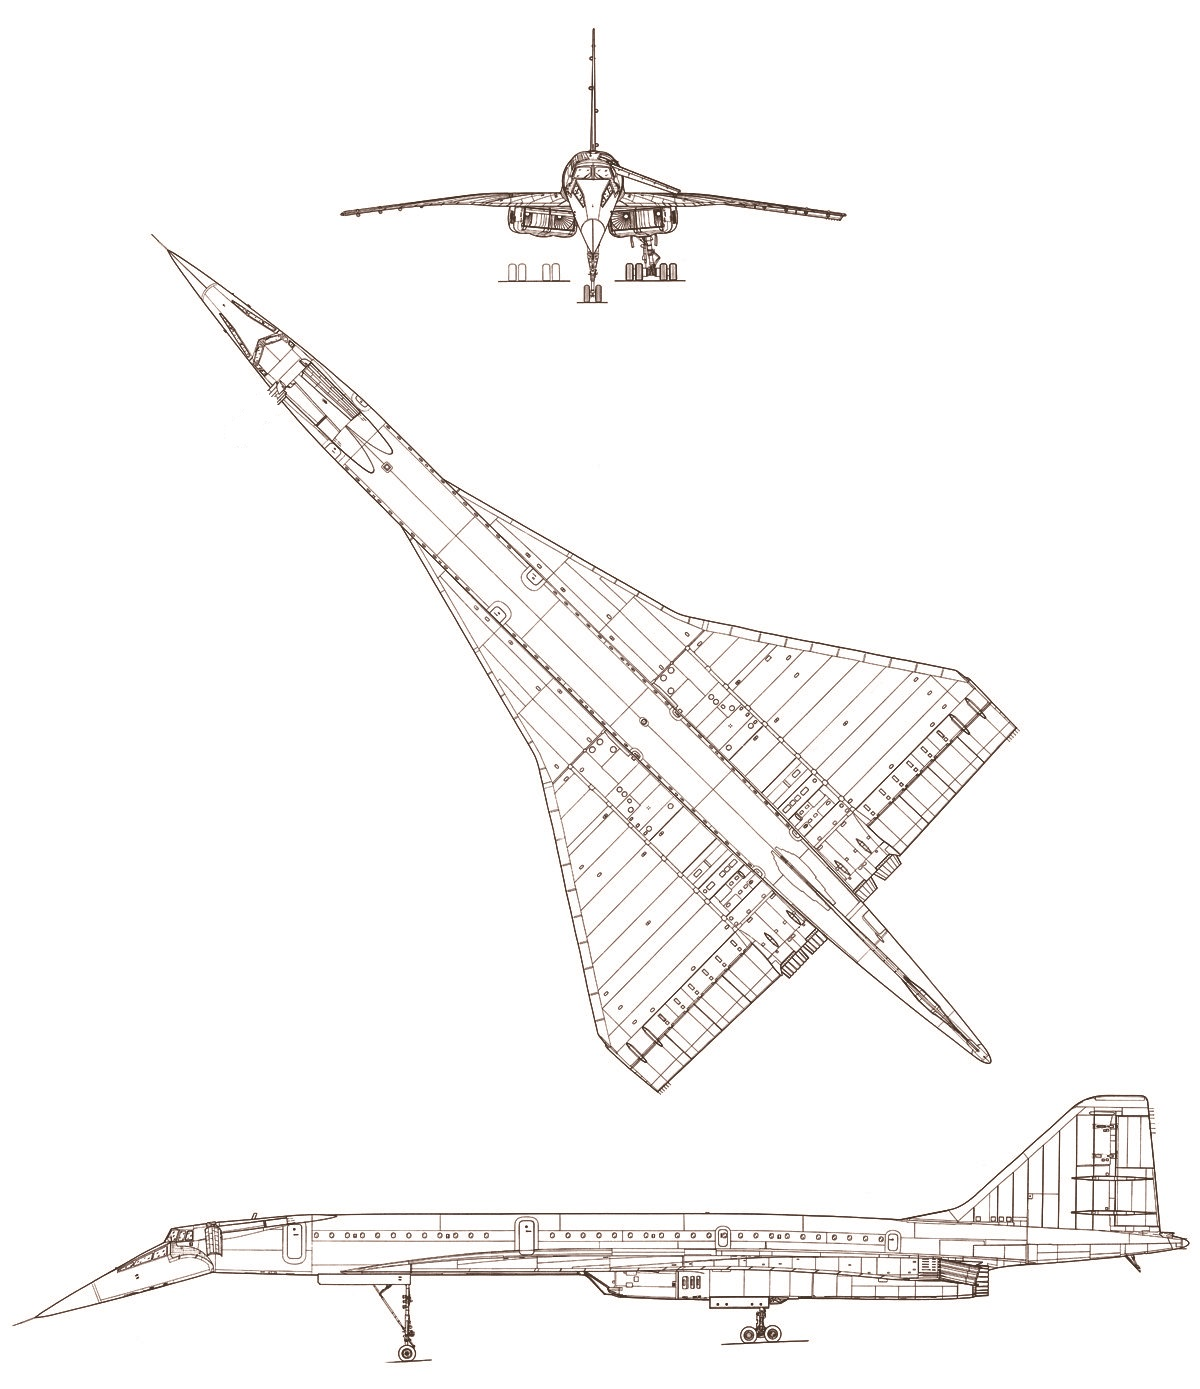
\includegraphics[width=\linewidth]{img/Concorde.jpg}}
    \caption{Concorde}
    \label{fig:Concorde}
\end{figure}
\newpage
\section{Исходные данные}
\pagestyle{fancy}
\fancyhf{}
\rhead{Дипломная работа}
\lhead{Исходные данные}
\rfoot{\thepage}

\begin{longtable}[H]{|c|c|c|c|c|}
    \caption[Исходные данные]{Исходные данные} \label{tab:Исходные данные} \\
    \hline 
    №& Парамтр & Обозначение & Значение & Единица измерения\\ \hline
    \endfirsthead
    
    \multicolumn{5}{c}%
    {{ \tablename\ \thetable{}: Исходные данные}} \\
    \hline 
    №& Парамтр & Обозначение & Значение & Единица измерения\\ \hline
    \endhead
    \endfoot
    
    \hline \hline
    \endlastfoot
         \hline
        1 & Расчётная масса & $m$ & 180 & т\\ \hline
        2 & Масса пустова & $m_\text{пуст}$ & 80 & т\\
         & самолёта &  &  & \\ \hline
        3 & Масса топлива & $m_\text{т}$ & 90 & т\\ \hline
        4 & Масса комерческой & $m_\text{к}$ & 9 & т \\
         & нагрузки & & & \\ \hline
        5 & Площадь крыла & $S$ & 360 & м$^2$\\ \hline
        6 & Ширина хорды САХ & $b_a$& 14,5 & м\\ \hline
        7 & Размах крыла & $l$ & 25,6 & м\\ \hline
        8 & Стартовая тяга двигателя & $P_0$ & 180000 $\cdot 4$ & Н\\ \hline
        9 & Момент инерции самолёта& $J_z$ & 7,7 $\cdot 10^{6}$ & кг $\cdot$ м$^2$ \\ 
         & относительно оси OZ &  &  & \\ \hline
        10 & Эксплуатационная вертикальная & $n_y^\text{э}$ & 3,5 & -\\ 
         & перегрузка &  &  & \\ \hline
        11 & Максимальное значение & $q_{max}$ & $5 \cdot 10^5$ & Н/м$^2$\\ 
         & скоростного напора &  &  & \\ \hline
        12 & Предельное значение & $M_\text{пред}$ & 2,4 & -\\ 
         & числа Маха &  &  & \\ \hline
        13 & Относительное значение & $\bar{X}_{T}$ & 0,25& -\\ 
         & центровки самолёта &  &  & \\ \hline
        14 & Максимальный угол отклонения & $\delta_{\text{э}_{max}}$ & 25 &град \\ 
        & элевонов & & & \\ \hline
        15 & Нагрузка на крыло & $P_s$ & 4905 & ${\text{Н}}/{\text{м}^2}$ \\ \hline
        16 & Тяговооруженность & $\bar{P}_0$ & 0,408 & - \\ \hline

\end{longtable}

\begin{table}[H]
    \centering
    \caption{Коэффициенты, характеризующие продольное движение}
    \label{tab:Коэффициенты, характеризующие продольное движение}
    \begin{tabular}{|c||c|c|c|c|c|}
    \hline
        $M$ & $C_{y_0}^{\delta \text{э}}$ &$X_F$ & $X_{F_{\text{э}}}$ &$m_z^{\bar{\omega}_z}$ & $C_y^{\alpha}$ \\ \hline \hline
        0,03  & 0,8  & 0,285  & 0,6  & -3,25 & 2,3 \\ \hline
        0,25  & 0,8  & 0,285  & 0,6  & -3,25 &2,3 \\ \hline
        0,5  & 0,8  & 0,285  & 0,6  & -3,25 & 2,25\\ \hline
        0,75  & 0,8  & 0,288  & 0,6  & -3,36 & 2,26\\ \hline
        1  & 0,55  & 0,314  & 0,6  & -3,5 &2,28 \\ \hline
        1,25  & 0,45  & 0,39  & 0,76  & -3,3 &2,5 \\ \hline
        1,5  & 0,43  & 0,45  & 0,86  & -3,05 &2,97 \\ \hline
        1,75  & 0,43  & 0,45  & 0,86  & -2,9 & 3\\ \hline
        2  & 0,445  & 0,446  & 0,86  & -2,8 & 2,82\\ \hline
        2,25  & 0,44  & 0,44  & 0,86  & -2,75 & 2,75\\ \hline
        2,5  & 0,42  & 0,43  & 0,86  & -2,74 & 2,68\\ \hline
        2,75  & 0,38  & 0,43  & 0,86  & -2,74 & 2,61\\ \hline
        3  & 0,35  & 0,43  & 0,86  & -2,74 & 2,54\\ \hline
    \end{tabular}
\end{table}

\begin{table}[H]
    \centering
    \caption{Аэродинамичекские характеристики }
    \label{tab:Аэродинамичекские характеристики }
    \begin{tabular}{|c||c|c|c|c|}
    \hline
        $M$  & $A$  & $C_{x_{m}}$  & $C_y^{\text{доп}}$  & $C_y^{\alpha}$   \\ \hline \hline
        0,03  & 0,025  & 0,0175  & 0,85  & 2,3   \\ \hline
        0,25  & 0,025  & 0,0175  & 0,85  & 2,3  \\ \hline
        0,5  & 0,0247  & 0,01755  & 0,85  & 2,25  \\ \hline
        0,75  & 0,0242  & 0,0175655  & 0,84  & 2,26  \\ \hline
        1  & 0,0237  & 0,018  & 0,75  & 2,28  \\ \hline
        1,25  & 0,0256  & 0,0192  & 0,7  & 2,5   \\ \hline
        1,5  & 0,034  & 0,0223  & 0,65  & 2,97  \\ \hline
        1,75  & 0,038  & 0,022  & 0,63  & 3  \\ \hline
        2  & 0,042  & 0,02185  & 0,61  & 2,82   \\ \hline
        2,25  & 0,0445  & 0,0216  & 0,6  & 2,75   \\ \hline
        2,5  & 0,0475  & 0,0215  & 0,59  & 2,68  \\ \hline
        2,75  & 0,0498  & 0,02155  & 0,53  & 2,61   \\ \hline
        3 & 0,0498  & 0,0215  & 0,51  & 2,54   \\ \hline
    \end{tabular}
\end{table}

\begin{figure}[H]
    \center{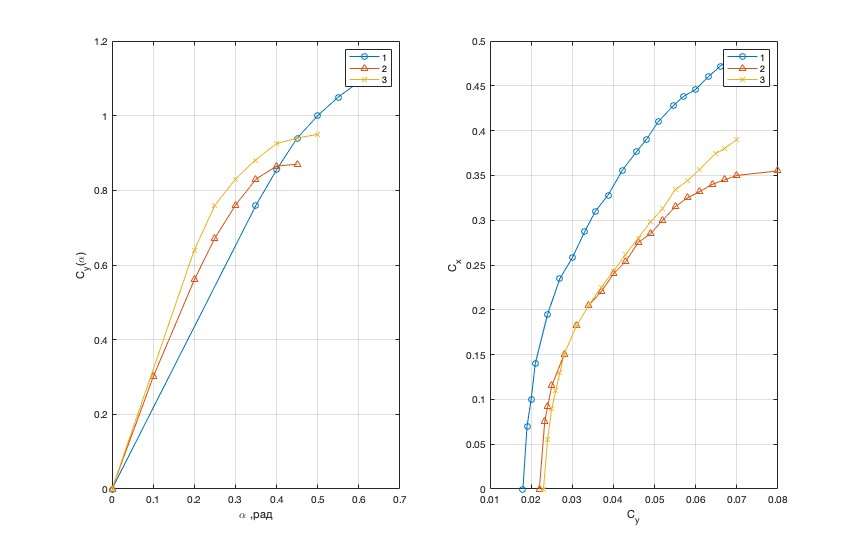
\includegraphics[width=\linewidth]{img/ПолярыДанные.jpg}}
    \caption{Аэродинамические характеристики на взлётно-посадочных
режимах;1-взлетный, 2-посадочный, 3-пробег с выпущенными
интерцепторами}
    \label{fig:ИД Взлёт посадка}
\end{figure}

\begin{center}
    Характеристики двигателя ДТРДФ:
\end{center}

\begin{longtable}[H]{|c|c|c|c|c|c|}
    \caption[Относительная тяга двигателя]{Относительная тяга двигателя, $\tilde{P}$} \label{tab:Относительная тяга двигателя} \\
    \hline 
    M/H, км& 0 & 3 & 6 & 9 &11 \\ \hline
    \endfirsthead
    
    \multicolumn{6}{c}%
    {{ \tablename\ \thetable{}: Относительная тяга двигателя, $\tilde{P}$}} \\
    \hline 
    M/H, км& 0 & 3 & 6 & 9 &11 \\ \hline
    \endhead
    \endfoot
    
    \hline \hline
    \endlastfoot
    \hline
        0,000  & 1,000 & 0,780 & 0,606 & 0,479 & 0,382  \\ \hline
        0,250  & 0,836 & 0,680 & 0,510 & 0,404 & 0,327  \\ \hline
        0,500  & 0,788 & 0,629 & 0,486 & 0,376 & 0,302  \\ \hline
        0,750  & 0,851 & 0,672 & 0,531 & 0,416 & 0,334  \\ \hline
        1,000  & 0,935 & 0,750 & 0,580 & 0,453 & 0,376  \\ \hline
        1,250  & 1,006 & 0,810 & 0,612 & 0,479 & 0,396  \\ \hline
        1,500  & 1,094 & 0,877 & 0,665 & 0,520 & 0,427  \\ \hline
        1,750  & 1,196 & 0,947 & 0,731 & 0,572 & 0,468  \\ \hline
        2,000  & 1,299 & 1,057 & 0,824 & 0,637 & 0,510  \\ \hline
        2,250  & 1,213 & 0,963 & 0,760 & 0,580 & 0,475  \\ \hline
        2,500  & 1,034 & 0,832 & 0,649 & 0,502 & 0,412  \\ \hline
        2,750  & 0,899 & 0,724 & 0,557 & 0,427 & 0,352  \\ \hline
        3,000  & 0,850 & 0,650 & 0,490 & 0,370 & 0,490  \\ \hline
\end{longtable}

\begin{longtable}[H]{|c|c|c|c|c|c|}
    \caption{Удельный расход топлива $C_{e}(M,H),\frac{\text{кг}}{\text{кгс} \cdot \text{час}}$} \label{tab:Удельный расход топлива} \\
    \hline 
    M/H, км& 0 & 3 & 6 & 9 &11 \\ \hline
    \endfirsthead
    
    \multicolumn{6}{c}%
    {{ \tablename\ \thetable{}: Удельный расход топлива $C_{e}(M,H),\frac{\text{кг}}{\text{кгс} \cdot \text{час}}$}} \\
    \hline 
    M/H, км& 0 & 3 & 6 & 9 &11 \\ \hline
    \endhead
    \endfoot
    
    \hline \hline
    \endlastfoot
    \hline
        0  & 0,88434 & 0,845814545 & 0,807289091 & 0,768763636 & 0,74308  \\ \hline
        0,25  & 0,9226 & 0,883673636 & 0,844747273 & 0,805820909 & 0,77987  \\ \hline
        0,5  & 0,9844 & 0,942263636 & 0,900127273 & 0,857990909 & 0,8299  \\ \hline
        0,75  & 1,07122 & 1,023866364 & 0,976512727 & 0,929159091 & 0,89759  \\ \hline
        1  & 1,16 & 1,12 & 1,068142727 & 1,014369091 & 0,97852  \\ \hline
        1,25  & 1,23161 & 1,184256364 & 1,136902727 & 1,089549091 & 1,05798  \\ \hline
        1,5  & 1,29341 & 1,24445 & 1,19549 & 1,14653 & 1,11389  \\ \hline
        1,75  & 1,33755 & 1,286585455 & 1,235620909 & 1,184656364 & 1,15068  \\ \hline
        2  & 1,38022 & 1,32805 & 1,27588 & 1,22371 & 1,18893  \\ \hline
        2,25  & 1,407 & 1,348786364 & 1,298222727 & 1,247659091 & 1,21395  \\ \hline
        2,5  & 1,42437 & 1,373402727 & 1,322435455 & 1,271468182 & 1,23749  \\ \hline
        2,75  & 1,43614 & 1,38718 & 1,33822 & 1,28926 & 1,25662  \\ \hline
        3 & 1,44 & 1,39 & 1,34 & 1,294 & 1,26 \\ \hline
\end{longtable}

\begin{figure}[H]
    \center{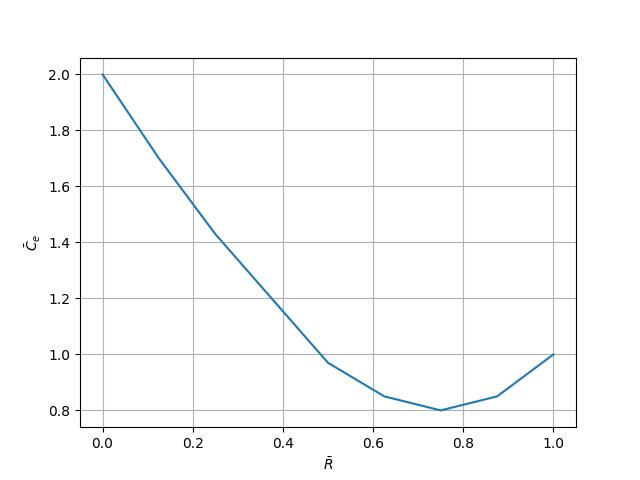
\includegraphics[width=\linewidth]{img/Дроссель.jpg}}
    \caption{Зависимость $\bar{C}_{e}(\bar{R})$}
    \label{fig:Ce}
\end{figure}

\begin{center}
    Выводы:
\end{center}

 Вся необходимая информация, необходимая для расчетов ЛТХ, ВПХ, траектории полета, транспортных возможностей самолет, маневренных характеристик и т.д., были получены из альбома
 исходнных данных кафедры. В результате анализа этих исходных данных был сделан вывод, что корректировка или дополнение исходных сведений не требуется. 


% Все исходные данные, необходимые для расчетов, были взяты из
% альбома исходных данных кафедры. Полученных данных достаточно для проведения всех необходимых расчетов. Корректировка и дополнение исходных данных не требуется.



\section{Первый курсач}

\begin{frame}{Расчёт ЛТХ}
\begin{block}{В расчёт ЛТХ входит}
   \begin{enumerate}
    \item [] <+->
    \item <+-> Расчёт области возможных полётов
    \item <+-> Расчёт траектории полёта 
    \item <+-> Расчёт транспортных возможностей самолёта
   \end{enumerate}
\end{block}
\end{frame}

\begin{frame}{Расчёт области возможных полётов}

    \begin{block}{Основные ограничения}
        \begin{itemize}
            \item Ограничение по $M_{min \ P}$ 
            \item Ограничение по $M_{max \ P}$
        \end{itemize}
    \end{block}

    \begin{block}{Дополнительные ограничения}
        \begin{itemize}
            \item Ограничение по $C_{y \ \text{доп}}$
            \item Ограничение по $M_\text{пред}$
            \item Ограничение по $q_{maxs}$
        \end{itemize}
    \end{block}

\end{frame}

\begin{frame}{Расчёт области возможных полётов}
    \begin{minipage}[c]{0.55\textwidth}
        \center{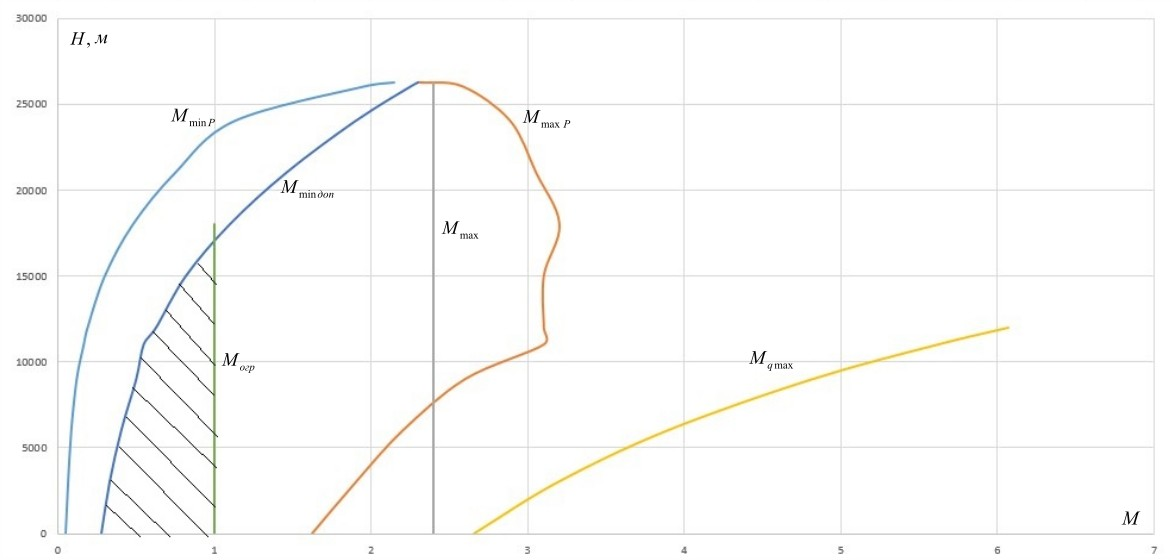
\includegraphics[width=6cm, height = 7cm]{../Оглавление/Part1/figures/Область.jpg}}
    \end{minipage}
    \begin{minipage}[c]{0.4\textwidth}
        \begin{itemize}
            \item <+-> []
            \item <+-> [] \begin{block}{Определение области}
                \begin{itemize}
                    \item $M_{min} = max \{ M_{min \ p}, \ M_{C_{y \ \text{доп}}} \} $
                    \item $M_{max} = min \{ M_{max \ P}, \ M_{\text{пред}}, \ M_{q_{max}} \}$
                \end{itemize}
            \end{block}
        \end{itemize}
    \end{minipage}
\end{frame}

\begin{frame}{Определение теоретического и практического потолка}
    \begin{minipage}[c]{0.45\textwidth}
        \begin{block}{Потолки}
        \begin{itemize}
            \item <+-> []
            \item <+-> [] Расчёт теоретического и практического потолка производится по $V_{y_{max}}$
            \item <+-> [] $H_\text{т} = 19,8$ км 
            \item <+-> [] $H_\text{пр} = 19,5$ км
        \end{itemize}
        \end{block}
    \end{minipage}
    \begin{minipage}[c]{0.45\textwidth}
        \center{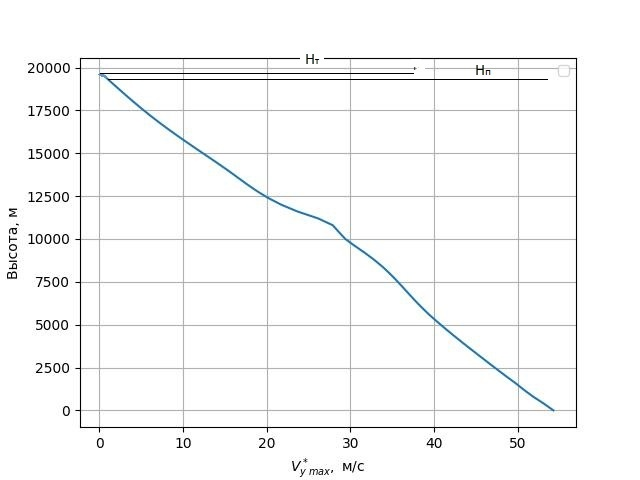
\includegraphics[width=6cm, height = 7cm]{../Оглавление/Part1/figures/Vy(H).jpg}}
    \end{minipage}
\end{frame}

\begin{frame}{Расчёт траектории полёта}
    \begin{block}{Траектория}
    \begin{itemize}
        \item [] <+->
        \item [] <+-> Траеткорию полёта принято разделять на три этапа 
            \begin{itemize}
                \item Набор высоты 
                \item Крейсерский полёт 
                \item Снижение 
            \end{itemize}
    \end{itemize}
    \end{block}
\end{frame}
\subsection{Расчет траектории полета}

В данном разделе была рассчитана траектория полета самолета-прототипа
Concorde. Траектория полета включает в себя следующие участки: набор высоты,
крейсерский полет, снижение. Ниже приведены формулы и соотношения,
которые были использованы при расчете

\subsubsection{Расчётные формулы и соотношения}
\label{sec:Расчётные формулы и соотношения}

\begin{center}
    Набор высоты:
\end{center}

Программа набора высоты, 1/с -- 
\begin{equation}
\label{eq:Программа набора}
    V' = \frac{dV}{dt} = \frac{V^{i+1}+V^{i}}{H^{i+1}+H^{i}}
\end{equation}

Коэффициент, используемый для расчета характеристик набора и снижения --  
\begin{equation}
    \label{eq:Коэффициент}
    \kappa = \frac{1}{\frac{V'V}{g}+1}
\end{equation}

Тангенциальная перегрузка --  
\begin{equation}
    \label{eq:Тангенциальная перегрузка }
    n_x = \frac{P\text{р}-P\text{п}}{mg}
\end{equation}

Угол набора высоты, град -- 
\begin{equation}
    \label{eq:Угол набора высоты}
    \theta_\text{наб} = n_x \cdot \kappa \cdot \frac{180^0}{\pi}
\end{equation}

Энергетическая скороподъемность, м/c -- 
\begin{equation}
    \label{eq:Энергетическая скороподъемность}
    V_y^* = V \cdot n_x
\end{equation}

Вертикальная скорость на участке набора высоты, м/с
\begin{equation}
    \label{eq:Вертикальная скорость на участке набора высоты}
    V_{y_\text{наб}} = V_y^* \cdot \kappa
\end{equation}

Дальность участка набора высоты, км -- 
\begin{equation}
    \label{eq:Дальность участка набора высоты}
    L_\text{наб} = \int_{H_\text{эк}}^{H_\text{эн}}\frac{dH_\text{э}}{1000 n_x}
\end{equation}

Время участка набора высоты, мин -- 
\begin{equation}
    \label{eq:Время участка набора высоты}
    t_\text{наб} = \int_{H_\text{эк}}^{H_\text{эн}}\frac{dH_\text{э}}{V_y^* 60}
\end{equation}

Масса топлива, расходуемого за участок набора, кг -- 
\begin{equation}
    \label{eq:Масса топлива, расходуемого за участок набора}
    m_T{_\text{наб}} = \int_{H_\text{эк}}^{H_\text{эн}}\frac{dH_\text{э}}{3600} \cdot \frac{C_eP_\text{р}}{V_y^*}
\end{equation}

\begin{center}
    Крейсерский полёт:
\end{center}

Относительный расход топлива -- 
\begin{equation}
    \label{eq:Относительный расход топлива}
    \bar{m}_{T_\text{кр}} = 1-\bar{m}_\text{сн}-\bar{m}_\text{цн} - \bar{m}_{T_\text{наб}} - \bar{m}_{T_\text{снп}} - \bar{m}_{T_\text{анз}} - \bar{m}_{T_\text{пр}}
\end{equation}

Время крейсерского полёта, мин -- 
\begin{equation}
    \label{eq:Время крейсерского полёта}
    T_\text{кр} = \frac{60 K_\text{ГП}}{g \cdot C_e} \ln{\frac{1 - \bar{m}_{T_\text{наб}} - \bar{m}_{T_\text{пр}}}{1 - \bar{m}_{T_\text{кр}} - \bar{m}_{T_\text{наб}} - \bar{m}_{T_\text{пр}}}}
\end{equation}

Дальность крейсерского полёта, км -- 
\begin{equation}
    \label{eq:Дальность крейсерского полёта}
    L_\text{кр} = \frac{3,6 V K_\text{ГП}}{g \cdot C_e} \ln{\frac{1 - \bar{m}_{T_\text{наб}} - \bar{m}_{T_\text{пр}}}{1 - \bar{m}_{T_\text{кр}} - \bar{m}_{T_\text{наб}} - \bar{m}_{T_\text{пр}}}}
\end{equation}

Плотность воздуха на высоте, кг/м$^3$
\begin{equation}
    \label{eq:Плотность воздуха на высоте}
    \rho_\text{нкр} = \frac{2 \bar{m}_\text{ккр}Ps10}{C_{y_\text{ГП}}V_\text{к}^2}
\end{equation}

\begin{center}
    Снижение:
\end{center}

Дальность участка снижения высоты, км -- 
\begin{equation}
    \label{eq:Дальность участка снижения высоты}
    L_\text{сн} = \int_{H_\text{эк}}^{H_\text{эн}}\frac{dH_\text{э}}{1000 n_x}
\end{equation}

Время участка снижения высоты, мин -- 
\begin{equation}
    \label{eq:Время участка снижения высоты}
    t_\text{сн} = \int_{H_\text{эк}}^{H_\text{эн}}\frac{dH_\text{э}}{V_y^* 60}
\end{equation}

Масса топлива, расходуемого за участок снижения, кг -- 
\begin{equation}
    \label{eq:Масса топлива, расходуемого за участок снижения}
    m_T{_\text{сн}} = \int_{H_\text{эк}}^{H_\text{эн}}\frac{dH_\text{э}}{3600} \cdot \frac{C_eP_\text{р}}{V_y^*}
\end{equation}

\subsubsection{Расчет характеристик набора высоты}

В начале расчета необходимо определить H, М в начале набора высоты и
H, М в конце набора высоты.

Начальные значения H и М определяются следующим образом $H_0 = 0 $ км $M_0 = 1,2 \cdot M_{min \text{доп}}$,а конечные значения выбираются из условия минимума километрового расхода топлива в установившемся горизонтальном полете. Высота и число Маха, при которых километровый расход топлива принимает наименьшее значение, определены в предыдущем разделе (см. раздел \ref{sec:Результаты расчета летно-технических характеристик
самолета-прототипа Concorde},таблица \ref{tab:Основные ограничения на область полётов}) 

При наборе высоты режим работы двигателя - "максимал". 

Учитывая сказанное выше, получаем:
\begin{itemize}
    \item [-] Начало набора высоты: $H_0 = 0$ км, $M_0 = 1,2 \cdot 0,276 = 0,3312$
    \item [-] Окончание набора высоты: $H_\text{к} = 10,8$ км, $M_\text{к} = 0,8$
\end{itemize}

В качестве программы принимается полученная в разделе \ref{sec:Результаты расчета летно-технических характеристик самолета-прототипа Concorde} зависимость $M_\text{наб}(M)$ соответствующая максимальной энергетической скороподъемности. Данная программа близка к оптимальным программам набора высоты по критериям минимума расхода топлива или набора времени. 

Зная программу набора высоты можно найти её характеристики: угол наклона траектории $\theta_\text{наб}$, вертикальная скорость $V_{y_\text{наб}}$, время $t_\text{наб}$ , дальность $L_\text{наб}$, расход топлива $M_{T_\text{наб}}$, они определяются по формулам \ref{eq:Программа набора}-\ref{eq:Масса топлива, расходуемого за участок набора}. Результаты расчетов характеристик набора высоты оформлены в виде таблицы (см.таблицу \ref{tab:Результаты расчета характеристик набора высоты}) 

\begin{longtable}[H]{|c|c|c|c|c|c|c|c|}
    \caption{Результаты расчета характеристик набора высоты} \label{tab:Результаты расчета характеристик набора высоты} \\
    \hline 
    H, м& $M$ & $V$, м/с & $n_x$ & $V_y^*$, м/c & $H_\text{э}$, м & $C_e$, кг/($H \cdot$ ч) & $P_\text{п}$\\ \hline
    \endfirsthead
    
    \multicolumn{8}{c}%
    {{ \tablename\ \thetable{}: Результаты расчета характеристик набора высоты}} \\
    \hline 
    H, км& $M$ & $V$, м/с & $n_x$ & $V_y^*$, м/c & $H_\text{э}$ &, м $C_e$, кг/($H \cdot$ ч) & $P_\text{п}$\\ \hline
    \endhead
    \endfoot
    
    \hline \hline
    \endlastfoot
    \hline
    0 & 0.33 & 112.74 & 0.3 & 34.0 & 647.83 & 0.9399 & 74133.0 \\ \hline 1000 & 0.37 & 124.71 & 0.28 & 34.53 & 1792.64 & 0.9365 & 77157.0 \\ \hline 2000 & 0.4 & 133.75 & 0.25 & 33.57 & 2911.71 & 0.9306 & 78395.0 \\ \hline 3000 & 0.43 & 140.73 & 0.23 & 31.75 & 4009.48 & 0.9234 & 78396.0 \\ \hline 4000 & 0.45 & 147.41 & 0.2 & 29.75 & 5107.59 & 0.916 & 77976.0 \\ \hline 5000 & 0.48 & 154.9 & 0.18 & 27.98 & 6223.01 & 0.9095 & 77670.0 \\ \hline 6000 & 0.52 & 163.05 & 0.16 & 26.6 & 7354.99 & 0.904 & 77382.0 \\ \hline 7000 & 0.55 & 171.59 & 0.15 & 25.59 & 8500.7 & 0.8996 & 76984.0 \\ \hline 8000 & 0.59 & 180.91 & 0.14 & 24.71 & 9668.18 & 0.8959 & 76588.0 \\ \hline 9000 & 0.63 & 191.09 & 0.12 & 23.51 & 10861.06 & 0.8921 & 76216.0 \\ \hline 10000 & 0.67 & 201.03 & 0.11 & 21.62 & 12059.82 & 0.8874 & 75512.0 \\ \hline 11000 & 0.71 & 209.3 & 0.1 & 20.07 & 13232.68 & 0.8853 & 74205.0
    
        
\end{longtable}


\begin{longtable}[H]{|c|c|c|c|c|c|c|}
    \caption{Результаты расчета характеристик набора высоты} \label{tab:Результаты расчета характеристик набора высоты} \\
    \hline 
    H, м & $V'$, 1/с & $\theta_\text{наб}$, град& $V_{y_\text{наб}}$, м/c& $\Delta H_\text{э}$, м& $1/n_{x_\text{ср}}$&$1/V^*_{y_\text{наб}}$, c/м\\ \hline
    \endfirsthead
    
    \multicolumn{6}{c}%
    {{ \tablename\ \thetable{}: Результаты расчета характеристик набора высоты}} \\
    \hline 
    H, м & $V'$, 1/с & $\theta_\text{наб}$, град& $V_{y_\text{наб}}$, м/c& $\Delta H_\text{э}$, м& $1/n_{x_\text{ср}}$&$1/V^*_{y_\text{наб}}$, c/м\\ \hline
    \endhead
    \endfoot
    
    \hline \hline
    \endlastfoot
    \hline
    0 & 0.012 & 15.19 & 29.9 & 1144.7 & 3.464 & 0.03 \\ \hline 1000 & 0.0091 & 14.23 & 30.96 & 1119.2 & 3.798 & 0.03 \\ \hline 2000 & 0.007 & 13.13 & 30.64 & 1097.9 & 4.209 & 0.03 \\ \hline 3000 & 0.0067 & 11.8 & 28.98 & 1097.9 & 4.695 & 0.03 \\ \hline 4000 & 0.0075 & 10.4 & 26.75 & 1114.9 & 5.246 & 0.03 \\ \hline 5000 & 0.0082 & 9.17 & 24.78 & 1132.5 & 5.833 & 0.04 \\ \hline 6000 & 0.0087 & 8.17 & 23.25 & 1147.9 & 6.418 & 0.04 \\ \hline 7000 & 0.0092 & 7.36 & 22.06 & 1165.3 & 7.014 & 0.04 \\ \hline 8000 & 0.0097 & 6.64 & 20.95 & 1184.1 & 7.725 & 0.04 \\ \hline 9000 & 0.0104 & 5.86 & 19.51 & 1207.5 & 8.713 & 0.04 \\ \hline 10000 & 0.011 & 5.03 & 17.64 & 1231.5 & 9.849 & 0.05 \\ \hline 11000 & 0.0147 & 4.18 & 15.48 & 1328.4 & 11.881 & 0.05 \\ \hline 12000 & 0.0153 & 3.17 & 12.54 & 1364.3 & 14.714 & 0.06 \\ \hline 13000 & 0.0166 & 2.53 & 10.68 & 1424.3 & 17.624 & 0.07 \\ \hline 14000 & 0.0186 & 2.0 & 9.05 & 1507.5 & 21.65 & 0.08 \\ \hline 15000 & 0.0192 & 1.54 & 7.45 & 1561.3 & 28.284 & 0.1 \\ \hline 16000 & 0.018 & 1.14 & 5.91 & 1560.6 & 40.05 & 0.13
    
\end{longtable}

\begin{figure}[H]
    \center{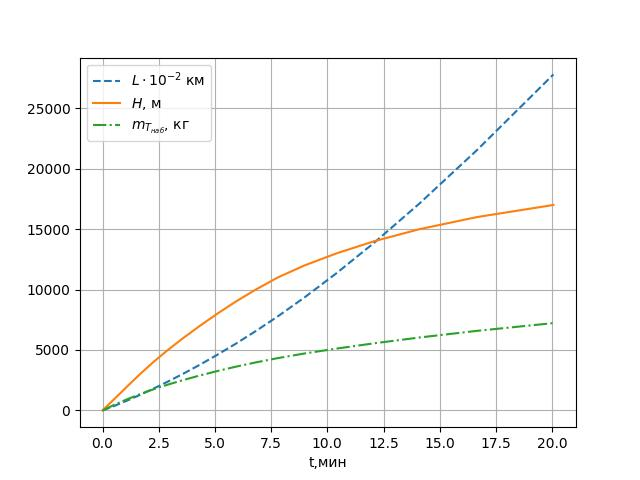
\includegraphics[width=\linewidth]{Оглавление/Part1/figures/Характеристики набора высоты1.jpg}}
    \caption{Характеристики набора высоты}
    \label{fig:Характеристики набора высоты1}
\end{figure}

\begin{figure}[H]
    \center{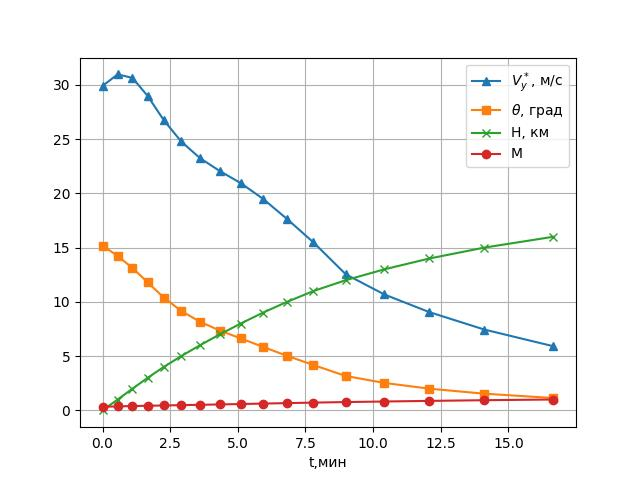
\includegraphics[width=\linewidth]{Оглавление/Part1/figures/Характеристики набора высоты2.jpg}}
    \caption{Характеристики набора высоты}
    \label{fig:Характеристики набора высоты2}
\end{figure}

\begin{table}[H]
    \centering
    \caption{Конечные результаты расчета параметров набора}
    \begin{tabular}{|c|c|}
    \hline
        Параметр & Значение \\ \hline
        $m_{T_\text{наб}}$ & 4310,3 кг\\ \hline
        $L_\text{кр}$ & 77,2 км\\ \hline
        $T_\text{кр}$ & 13,63 мин\\ \hline
    \end{tabular}
    \label{tab:Крейсер}
\end{table}


\subsubsection{Расчет характеристик крейсерского полета}
\label{sec: Расчет характеристик крейсерского полета}

В данном подразделе необходимо определить дальность и
продолжительность крейсерского полета, последовательность расчетов
изложена далее.
Относительный расход топлива на участке крейсерского полета вычисляется
при максимальной целевой (полезной) нагрузке для неманевренного самолета
по формуле \ref{eq:Относительная масса пустого снаряженного самолета}: 

\begin{equation}
    \label{eq:Относительная масса пустого снаряженного самолета}
    \bar{m}_{T_\text{кр}} = 1 - \bar{m}_{\text{цн}} - \bar{m}_{T_\text{наб}} - \bar{m}_{T_\text{снп}} - \bar{m}_{T_\text{анз}} - \bar{m}_{T_\text{пр}}
\end{equation}
$\bar{m}_{T_\text{сн}} = 0,5$ -- относительная масса пустого снаряженного самолета \\ 
$\bar{m}_{\text{цн}} = 0,15$ -- относительная масса целевой нагрузки \\ 
$\bar{m}_{T_\text{снп}} = 0,015$ -- относительная масса топлива, расходуемая при снижении и
посадке \\ 
$\bar{m}_{T_\text{наб}}$ --  относительная масса топлива,
расходуемая при наборе высоты \\

Используя формулы из раздела \ref{sec:Расчётные формулы и соотношения} расчитаем: 

\begin{itemize}
    \item [-] высоту конца крейсерского полёта $H_{\text{к} \ \text{кр}}$
    \item [-] дальность крейсерского полёта $L_\text{кр}$
    \item [-] продолжительность полёта $T_\text{кр}$
\end{itemize}
Все данные приведены в таблице (\ref{tab:Крейсер})

\begin{table}[H]
    \centering
    \caption{Конечные результаты расчетов}
    \begin{tabular}{|c|c|}
    \hline
        Параметр & Значение \\ \hline
        $H_{\text{к} \ \text{кр}}$ & 12,300 км\\ \hline
        $L_\text{кр}$ & 5910 кг\\ \hline
        $T_\text{кр}$ & 470 мин\\ \hline
    \end{tabular}
    \label{tab:Крейсер}
\end{table}


\subsubsection{Расчет характеристик снижения}

В данном подразделе производится расчет следующих характеристик
снижения: угол наклона траектории $\theta_\text{сн}$, вертикальная скорость $V_{y_\text{сн}}$, время $t_\text{сн}$ ,дальность $L_\text{сн}$. Расчет проводится по формулам \ref{eq:Дальность участка снижения высоты}-\ref{eq:Масса топлива, расходуемого за участок снижения}, аналогичным расчету участка набора высоты. 

В качестве программы снижения принимается полученная в разделе \ref{sec:Результаты расчета летно-технических характеристик самолета-прототипа Concorde} зависимость $M_\text{сн}(H)$, соответствующая минимуму потребной тяги (максимальному аэродинамическому качеству). Данная программа близка к оптимальной программе снижения с точки зрения получения максимальной дальности полета. 
Программа снижения содержит два участка:
\begin{enumerate}
    \item торможение на высоте $H_\text{кр}$ до скорости $M(P_{\text{п} \ min})$
    \item снижение до высоты $H = 0$ км
\end{enumerate} 

При снижении режим работы двигателя - "малый газ". 

Высота начала снижения равна высоте полета самолета в конце крейсерского участка ($H_{0_\text{кр}} = H_\text{к \ кр}$) Число $M$(скорость $V$[км/ч]) полета соответствует минимуму потребной тяги на высоте $H_{0_\text{сн}}$, определяется по графику $M(P_{\text{п} \ min})$, построенному в разделе \ref{sec:Результаты расчета летно-технических характеристик самолета-прототипа Concorde}

Высота конца участка снижения условно принимается равной нулю ($H_\text{к \ сн}$). Скорость в конце снижения соответствует наивыгоднейшей скорости при $H = 0$ км, $M_\text{ксн}(P_{\text{п} \ min})$.  Исходя из вышесказанного, получим:
\begin{itemize}
    \item [-] Начальные условия: $H_{0 \ \text{сн}} = 11$ км, $M_{0 \ \text{сн}} 0,$
    \item [-] Конечные условия: $H_{\text{к} \ \text{сн}} = 0$ км, $M_{\text{к} \ \text{сн}}$
\end{itemize}

Все рассчитанные характеристики снижения занесены в таблицу \ref{tab: } 

\begin{longtable}[H]{|c|c|c|c|c|c|c|c|}
    \caption{Результаты расчета характеристик набора высоты} \label{tab:Результаты расчета характеристик набора высоты} \\
    \hline 
    H, м& $M$ & $V$, м/с & $n_x$ & $V_y^*$, м/c & $H_\text{э}$, м & $C_e$, кг/($H \cdot$ ч) & $P_\text{п}$\\ \hline
    \endfirsthead
    
    \multicolumn{8}{c}%
    {{ \tablename\ \thetable{}: Результаты расчета характеристик набора высоты}} \\
    \hline 
    H, км& $M$ & $V$, м/с & $n_x$ & $V_y^*$, м/c & $H_\text{э}$ &, м $C_e$, кг/($H \cdot$ ч) & $P_\text{п}$\\ \hline
    \endhead
    \endfoot
    
    \hline \hline
    \endlastfoot
    \hline
    11& 0.58 & 172.4 & -0.04 & -6.81 & 12514.81 & 0.1701 & 3325.0 \\ \hline 10 & 0.55 & 164.48 & -0.04 & -6.48 & 11378.89 & 0.1708 & 3649.0 \\ \hline 9 & 0.51 & 155.14 & -0.04 & -6.08 & 10226.69 & 0.1721 & 4070.0 \\ \hline 8 & 0.47 & 145.78 & -0.04 & -5.69 & 9083.15 & 0.1733 & 4457.0 \\ \hline 7 & 0.44 & 137.43 & -0.04 & -5.34 & 7962.63 & 0.1744 & 4826.0 \\ \hline 6 & 0.41 & 129.81 & -0.04 & -5.01 & 6858.8 & 0.1756 & 5239.0 \\ \hline 5 & 0.38 & 122.38 & -0.04 & -4.69 & 5763.35 & 0.177 & 5758.0 \\ \hline 4 & 0.36 & 115.59 & -0.04 & -4.39 & 4681.03 & 0.1785 & 6379.0 \\ \hline 3 & 0.33 & 109.97 & -0.04 & -4.13 & 3616.34 & 0.1803 & 7057.0 \\ \hline 2 & 0.32 & 105.13 & -0.04 & -3.91 & 2563.35 & 0.1821 & 7738.0 \\ \hline 1 & 0.3 & 100.28 & -0.04 & -3.69 & 1512.54 & 0.184 & 8368.0 \\ \hline 0 & 0.28 & 95.31 & -0.04 & -3.48 & 463.02 & 0.1857 & 8892.0
    
        
\end{longtable}


\begin{longtable}[H]{|c|c|c|c|c|c|c|}
    \caption{Результаты расчета характеристик набора высоты} \label{tab:Результаты расчета характеристик набора высоты} \\
    \hline 
    H, м & $V'$, 1/с & $\theta_\text{спуск}$, град& $V_{y_\text{спуск}}$, м/c& $\Delta H_\text{э}$, м& $1/n_{x_\text{ср}}$&$1/V^*_{y_\text{спуск}}$, c/м\\ \hline
    \endfirsthead
    
    \multicolumn{6}{c}%
    {{ \tablename\ \thetable{}: Результаты расчета характеристик набора высоты}} \\
    \hline 
    H, м & $V'$, 1/с & $\theta_\text{спуск}$, град& $V_{y_\text{спуск}}$, м/c& $\Delta H_\text{э}$, м& $1/n_{x_\text{ср}}$&$1/V^*_{y_\text{спуск}}$, c/м\\ \hline
    \endhead
    \endfoot
    
    \hline \hline
    \endlastfoot
    \hline
    11-10 & 0.0079 & -1.99 & -5.98 & -1135.9 & -25.347 & -0.15 \\ \hline 10-9 & 0.0093 & -1.95 & -5.6 & -1152.2 & -25.449 & -0.16 \\ \hline 9-8 & 0.0094 & -1.96 & -5.3 & -1143.5 & -25.567 & -0.17 \\ \hline 8-7 & 0.0083 & -1.99 & -5.06 & -1120.5 & -25.685 & -0.18 \\ \hline 7-6 & 0.0076 & -2.01 & -4.82 & -1103.8 & -25.817 & -0.19 \\ \hline 6-5 & 0.0074 & -2.02 & -4.57 & -1095.4 & -25.985 & -0.21 \\ \hline 5-4 & 0.0068 & -2.03 & -4.33 & -1082.3 & -26.201 & -0.22 \\ \hline 4000 & 0.0056 & -2.04 & -4.12 & -1064.7 & -26.458 & -0.23 \\ \hline 3-2 & 0.0048 & -2.04 & -3.92 & -1053.0 & -26.739 & -0.25 \\ \hline 2-1 & 0.0049 & -2.03 & -3.72 & -1050.8 & -27.016 & -0.26 \\ \hline 1-0 & 0.005 & -2.01 & -3.52 & -1049.5 & -27.264 & -0.28
    
\end{longtable}

\begin{figure}[H]
    \center{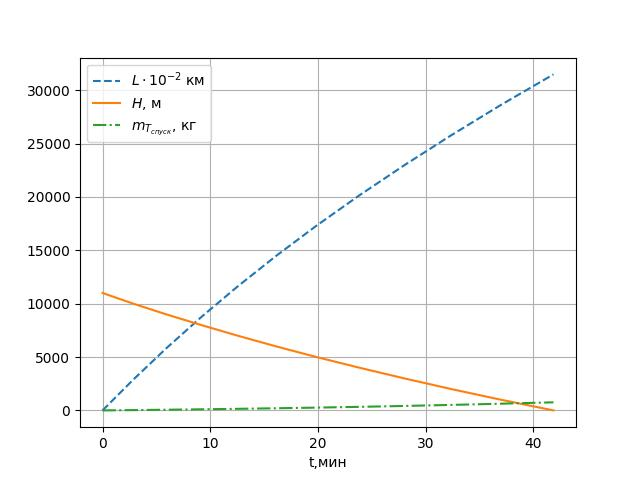
\includegraphics[width=\linewidth]{Оглавление/Part1/figures/Характеристики Спуска1.jpg}}
    \caption{Характеристики снижения}
    \label{fig:Характеристики Спуска1}
\end{figure}

\begin{figure}[H]
    \center{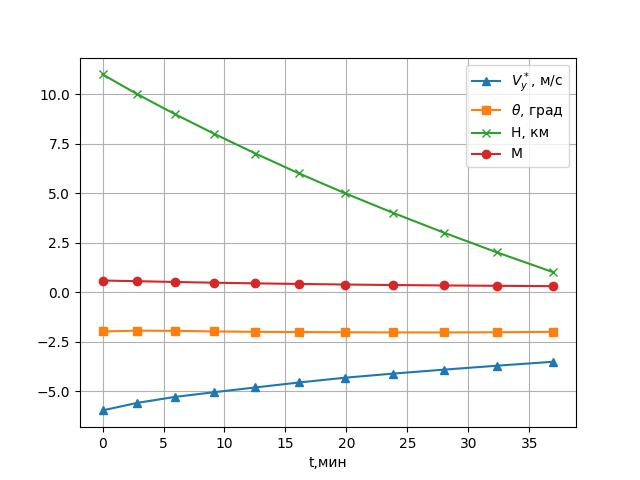
\includegraphics[width=\linewidth]{Оглавление/Part1/figures/Характеристики пуска2.jpg}}
    \caption{Характеристики снижения}
    \label{fig:Характеристики Спуска2}
\end{figure}

\begin{table}[H]
    \centering
    \caption{Конечные результаты расчета параметров набора}
    \begin{tabular}{|c|c|}
    \hline
        Параметр & Значение \\ \hline
        $m_{T_\text{наб}}$ & 757 кг\\ \hline
        $L_\text{кр}$ & 314,78 км\\ \hline
        $T_\text{кр}$ & 41,866 мин\\ \hline
    \end{tabular}
    \label{tab:Крейсер}
\end{table}

Зная, дальность набора высоты, крейсерского полета, снижения, высоту крейсерского полета, высоту конца крейсерского полета, рассчитанную траекторию полета можно представить графически (см. рис.\ref{fig:Траектория полёта}) 


\begin{figure}[H]
    \center{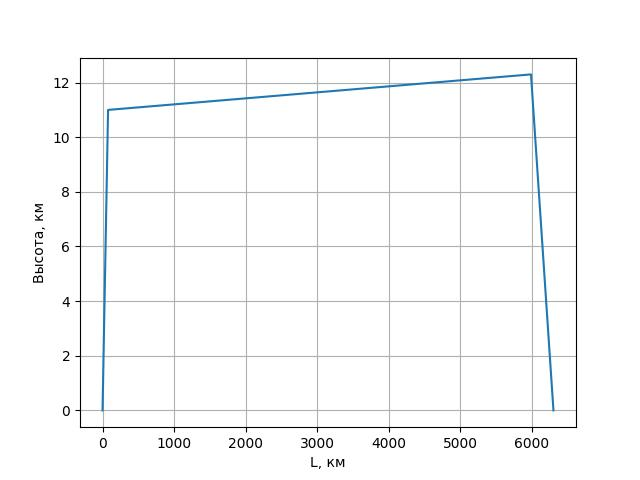
\includegraphics[width=\linewidth]{Оглавление/Part1/figures/Траектория полета.jpg}}
    \caption{Траектория полёта}
    \label{fig:Траектория полёта}
\end{figure}

Общая дальность полета и общая продолжительность полета равны:
\begin{itemize}
    \item [-] $L = 77,2 \text{ км} + 5909,75 \text{ км} + 314км = 6300\text{ км}$
    \item [-] $T = 12,3 \text{ мин} + 470,1 \text{ мин} + 41,86 \text{ мин} = 524,26 \text{ мин}$
\end{itemize}

\begin{center}
    Выводы:
\end{center}

После выполнения расчетов траектории полета самолета-прототипа Concorde
были получены следующие результаты:
\begin{itemize}
\item[-] общая дальность полета равна 6300 км
\item[-] общее время полета составляет 524,26 мин
\item[-] дальность набора высоты равна 77,2 км
\item[-] топливо, израсходованное на набор высоты равно 4310 кг
\item[-] время набора высоты равно 12,3 мин
\item[-] дальность снижения равна 314 км
\item[-] топливо, израсходованное на снижение равно 757 кг
\item[-] время снижения 41 мин
\end{itemize}
По вышеперечисленным результатам у данного самолета довольно большая
общая дальность полета, что позволяет ему совершать транспортировку
пассажиров на значительные расстояния 
\subsection{Расчет диаграммы транспортных возможностей неманевренного
самолета}
\label{sec:Расчет диаграммы транспортных возможностей неманевренного
самолета}
\pagestyle{fancy}
\fancyhf{}
\rhead{Дипломная работа}
\lhead{Расчёт транспортных возможностей}
\rfoot{\thepage}



\pagestyle{fancy}
\fancyhf{}
\rhead{Дипломная работа}
\lhead{Транспортные возможности самолёта}
\rfoot{\thepage}

Так как самолет Concorde предназначен для транспортировки пассажиров на различные расстояния, то необходимо знать его транспортные возможности, расчету которых и посвящен данный раздел. Ниже приведены формулы и соотношения, необходимые для проведения расчетов, а также пояснения к ним. 

\subsubsection{Расчетные формулы и соотношения}

Расчет ведется для трех режимов: 

\begin{enumerate}
    \item Полет с максимальной коммерческой нагрузкой
    \item Полет с максимальным запасом топлива
    \item Полет без коммерческой нагрузки ($m_\text{цн} = 0$) с максимальным запасом топлива
\end{enumerate}

\underline{Для режима №I} 

Дальность полета для данного режима определена в предыдущем подразделе (см. подраздел \ref{sec: Расчет характеристик крейсерского полета}) Относительная масса целевой нагрузки равна $\bar{m}_\text{цн}$ = хз. Для второго и третьего режимов дальность полета вычисляется по формуле $L = L_\text{наб} + L_\text{кр} + L_\text{сн}$. В целях упрощения расчетов принимается допущение, что дальности и расход топлива при наборе высоты ($L_\text{наб}$, $\bar{m}_{T_\text{наб}}$) и снижении ($L_\text{сн}$, $\bar{m}_{T_\text{сн}}$) для трех указанных режимов не изменяются. 

\underline{Для режима №II} 

Дальность полета для данного режима определяется по следующей формуле
(формула \ref{eq:Дальность крейсерского полёта})
$$\bar{m}_\text{взл} = \frac{m_\text{взл}}{m_0}$$
Зная параметры $V$, $K$, $C_e$, соответствующих крейсерскому
полету, принимаются равными вычисленным в подразделе \ref{sec: Расчет характеристик крейсерского полета}. Взлетная масса самолета $\bar{m}_\text{взл}$ и относительная масса топлива, затраченного на крейсерский полёт, $\bar{m}_{T_\text{кр}}$ определяется следующим образом:

$$\bar{m}_\text{взл} = 1$$
\begin{equation}
    \label{eq:Относительная масса топлива, затраченного на крейсерский полет}
    \bar{m}_{T_\text{кр}} = \bar{m}_{T_{max}} - \bar{m}_{T_\text{наб}} -\bar{m}_{T_\text{сн}} -\bar{m}_{T_\text{анз}} - \bar{m}_{T_\text{пр}}
\end{equation},
где $\bar{m}_{T_{max}}$ -- максимальная масса топлива, заливаемого в баки

Целевую нагрузку для данного режима можно определить следующим образом
\begin{equation}
    \label{eq:Целевая нагрузка}
    \bar{m}_\text{цн} = 1 - \bar{m}_\text{пуст} - \bar{m}_{T_{max}}
\end{equation}

\underline{Для режима №III}

Для данного режима полета дальность вычисляется согласно формуле для режима №II, а масса топлива определяется согласно формуле (\ref{eq:Относительная масса топлива, затраченного на крейсерский полет}). Относительная взлетная масса для данного режима полета равна:

\begin{equation}
    \label{eq:Относительная взлетная масса}
    \bar{m}_\text{взл} = \bar{m}_\text{пуст} + \bar{m}_{T_{max}} 
\end{equation}

\subsubsection{Результаты расчета транспортных возможностей самолета}
\label{sec:Результаты расчета транспортных возможностей самолета}

Согласно формулам \ref{eq:Относительная масса топлива, затраченного на крейсерский полет}-\ref{eq:Относительная взлетная масса},\ref{eq:Дальность крейсерского полёта} и вышеизложенным комментариям, были
проведены следующие вычисления:

\textbf{Режим №I}

Полет с максимальной коммерческой нагрузкой 
$$L = 77,2 \text{ км} + 5909,75 \text{ км} + 314 \text{ км} = 6300 \text{ км}$$
$$m_\text{цн} = m_0 \cdot \bar{m}_\text{цн} = 0,2 \cdot 180000 \text{ кг}= 36 000 \text{ кг}$$ 

\textbf{Режим №II}

Полет с максимальным запасом топлива 
$$\bar{m}_{T_\text{кр}} = 0,42 - 0,018 - 0,0032 - 0,05 - 0,01 = 0,3388$$
$$m_\text{цн} = 1 - 0,5 - 0,42 = 0,08$$
$$L_\text{кр} = 9954 \text{ км}$$
$$m_\text{цн} = m_0 \cdot \bar{m}_\text{цн} = 0,08 \cdot 180000 = 14400 \text{ кг}$$

\textbf{Режим №III}

Полет при максимальном запасе топлива без коммерческой нагрузки 
$$\bar{m}_{T_\text{кр}} 0 0,42 - 0,018 - 0,018 - 0,0032 - 0,05 - 0,01 = 0,3388$$
$$\bar{m}_\text{взл} = 0,5 + 0,42 = 0,92$$

$$L_\text{кр} = 11052,52$$
$$m_\text{цн} = m_0 \cdot \bar{m}_\text{цн} = 0 \text{ кг}$$

Вычисленные дальность полета и целевая нагрузка для режимов 1-3 занесены в
таблицу \ref{tab:Дальность полета и целевая нагрузка для режимов 1-3} 

\begin{table}[H]
    \centering
    \caption{Дальность полета и целевая нагрузка для режимов 1-3}
    \begin{tabular}{|c|c|c|c|}
    \hline
        Режим & I & II & III  \\ \hline
        $L$, км & 6300 & 9954 & 11052,52 \\ \hline
        $m_\text{цн}$, кг & 36 000 & 14400 &0 \\ \hline
    \end{tabular}
    \label{tab:Дальность полета и целевая нагрузка для режимов 1-3}
\end{table}

По данным таблицы \ref{tab:Дальность полета и целевая нагрузка для режимов 1-3}  была построена диаграмма транспортных возможностей для самолета-прототипа Concorde

\begin{figure}[H]
    \center{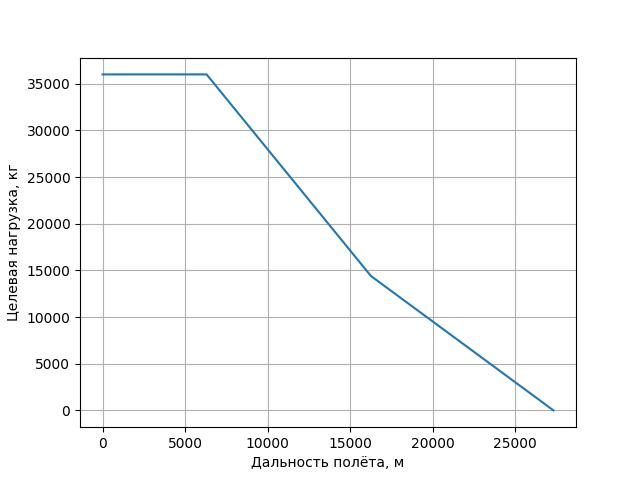
\includegraphics[width=\linewidth]{Оглавление/Part1/figures/Транспортные возможности.jpg}}
    \caption{Диаграмма транспортных возможностей неманевренного самолета Concorde (самолета –прототипа)}
    \label{fig:Диаграмма транспортных возможностей неманевренного самолета Concorde (самолета –прототипа)}
\end{figure}

\begin{center}
    Выводы:
\end{center}

Расчет транспортных возможностей показал следующие результаты:
\begin{enumerate}
    \item 6300 км- дальность полета с максимальной коммерческой нагрузкой
    \item 9954 гм- дальность полета с максимальным запасом топлива
    \item 11052,52 км-дальность полета при максимальном запасе топлива без
коммерческой нагрузки
\end{enumerate}

По данным результатам расчета самолет обладает хорошими транспортными
возможностями и может совершать полеты на значительные расстояния 



\subsection{Расчет взлетно-посадочных характеристик самолета}
\label{sec:Расчет взлетно-посадочных характеристик самолета}
\subsubsection{Расчетные формулы и соотношения}

Расчет взлетно-посадочных характеристик производится при следующих
предположениях: 
$\alpha_\text{р} = \alpha_\text{п} = 2^0$ -- угол атаки при разбеге и пробеге \\
$\alpha_\text{отр} = \alpha_\text{кас} = 6^0$ -- угол атаки при отрыве (во время взлёта) и качания ВПП (при пасадке).\\
$H_\text{взл} = 10,7$м, $H_\text{пос} = 15$м -- безопасная высота пролёта препятствий \\
$f_\text{р}$ -- коэффициент трения при разбеге \\
$f_\text{пр} = 0,2$ -- коэффициент трения при пробеге (с учётом тормозной системы), \\
тфга двигателя на взлётном режиме на 15...20\% больше наминальной тяги, при пробеге по ВПП на неманевренном самолёте используется режим "реверса тяги". \\

Скорость отрыва на взлёте -- 
\begin{equation}
    \label{eq:Скорость отрыва}
    V_\text{отр} = \sqrt{\frac{20P_s(1-0,9\bar{P}_\text{взл}\sin{\alpha_\text{отр}})}{\rho_0C_{y_\text{отр}}}}
\end{equation}

Длина разбега -- 
\begin{equation}
    \label{eq:Длина разбега}
    L_\text{р} = \frac{1}{2gb_\text{р}}\ln{\frac{C_\text{p}}{C_\text{р}-b_\text{р}V^2_\text{отр}}}
\end{equation}

Коэффициент тяги -- 
\begin{equation}
    \label{eq:Коэффициент тяги}
    C_\text{р} = 0,9 \bat{P}_\text{взл}-f_\text{р}
\end{equation}

Коэффициент при расчёте длины разега -- 
\begin{equation}
    \label{eq:Коэффициент при расчёте длины разега}
    b_\text{р} = (C_{x_\text{р}}-f_\text{р}C_{y_\text{р}})\frac{\rho_0}{2P_s10}
\end{equation}

Взлётная дистанция -- 
\begin{equation}
    \label{eq:Взлётная дистанция}
    L_\text{вд} = L_\text{р} + L_\text{вув}
\end{equation}

Длина воздушного участка взлёта
\begin{equation}
    \label{eq:Длина воздушного участка взлёта}
    L_\text{вув} = \frac{1}{\hat{n}_{x_\text{ср}}}(\frac{V_2^2-V^2_\text{отр}}{2g}+H_\text{взл})
\end{equation}

Среднеквадратичное значение скорости -- 
\begin{equation}
    \label{eq:Среднеквадратичное значение скорости}
    \hat{V}_\text{ср} = \sqrt{\frac{V_2^2-V^2_\text{отр}}{2}}
\end{equation}

Скорость качания ВПП -- 
\begin{equation}
    \label{eq:Скорость качания ВПП}
    V_\text{кас} = \sqrt{\frac{2\bar{m}_\text{пос}P_s10}{C_{y_\text{кас}}\rho_0}}
\end{equation}

Относительная масса -- 
\begin{equation}
    \label{eq:Относительная масса}
    \bar{m}_\text{пос} = \mkkr-\mtcnp
\end{equation}

Длина пробега -- 
\begin{equation}
    \label{eq:Длина пробега}
    L_\text{проб} = \frac{1}{2gb_\text{п}}\ln{\frac{a_\text{п}-b_\text{п}V^2_\text{кас}}{a_\text{п}}}
\end{equation}

Коэффициенты пробега -- 
\begin{equation}
    \label{eq:Коэффициент пробега1}
    a_\text{п} = -\bar{P}_\text{рев} - f_\text{п}
\end{equation}

\begin{equation}
    \label{eq:Коэффициент пробега2}
    b_\text{п} = \frac{\rho_0}{\bar{m}_\text{пос}P_s20}(C_{x_\text{проб}}-f_\text{п}C_{y_\text{проб}})
\end{equation}

Относительный реверс тяги на посадке -- 
\begin{equation}
    \label{eq:Относительный реверс тяги на посадке}
    \bar{P}_\text{рев} = \frac{P_\text{рев}}{m_\text{пос}g}
\end{equation}

Посадочная дистанция -- 
\begin{equation}
    \label{eq:Посадочная дистанция}
    L_\text{пд} = L_\text{проб} + L_\text{вуп}
\end{equation}

Длина воздушного участка посадки -- 
\begin{equation}
    \label{eq:Длина воздушного участка посадки}
        L_\text{вуп} = K_\text{пос}(\frac{V_\text{пл}^2-V^2_\text{кас}}{2g}+H_\text{пос})
\end{equation}
 
 Скорость планирования -- 
 \begin{equation}
     \label{eq:Скорость планирования}
     V_\text{пл} = \sqrt{\frac{2\bar{m}_\text{пос}P_s10}{C_{y_\text{пос}}\rho_0}}
 \end{equation}
 
 Аэродинамическое качество при посадке -- 
 \begin{equation}
     \label{eq:Аэродинамическое качество при посадке}
     K_\text{пос} = \frac{C_{y_\text{пос}}}{C_{x_\text{пос}}}
 \end{equation}
 
 \subsection{Результаты расчёта}
 
 \begin{table}[H]
     \centering
     \caption{Результаты расчета взлетно-посадочных характеристик самолета Concorde}
     \begin{tabular}{|c|c|c|c|c|c|}
     \hline
          $V_\text{отр}, $ м/c& $L_\text{р},$ м & $L_\text{вд},$ м& $V_\text{кас},$ м/с  &$L_\text{проб},$ м  &$L_\text{пд},$ м\\ \hline
          88,85& 1125,37 & 1392 & 64,58 & 576 &1200,78\\ \hline
     \end{tabular}
     \label{tab:my_label}
 \end{table}


  

\subsection{Расчет характеристик манёвренности самолета}
\label{sec:Расчёт характеристик манёвренности самолёта}
\pagestyle{fancy}
\fancyhf{}
\rhead{Дипломная работа}
\lhead{Расчёт манёвренных характеристик}
\rfoot{\thepage}

\subsubsection{Расчетные формулы и соотношения}

Для неманёвренного самолёта характеристики предельного правильного виража расчитываются для высоты $H = 6$км.

Характеристики маневренности рассчитываются при 50\%-ом выгорании топлива для
массы самолета: 

\begin{equation}
    \label{eq:Относительная масса смолёта}
    \bar{m}_c = 1-0,5\bar{m}_\text{т}
\end{equation}

Максимально допустимая нормальная перегрузка -- 
\begin{equation}
    \label{eq:Максимально допустимая нормальная перегрузка}
    n_{y_\text{доп}} = min \{n_{y_\text{э}},n_{y}(C_{y_\text{доп}}) \}
\end{equation}

\begin{equation}
    \label{eq:Эксплуатационная перегрузка}
    n_{y_\text{э}} = 2,5...3,5
\end{equation}

Допустимая нормальная перегрузка -- 
\begin{equation}
    \label{eq:Допустимая нормальная перегрузка}
    n_{y_\text{э}} = \frac{C_{y_\text{доп}}}{C_{y_\text{ГП}}}
\end{equation}

Коэффициент подъёмной силы горизонтального полёта --
\begin{equation}
    \label{eq:Коэффициент подъёмной силы горизонтального полёта}
    C_{y_\text{ГП}} = \frac{\bar{m}_cP_s10}{q}
\end{equation}

Нормальная перегрузка на вираже --
\begin{equation}
    \label{eq:Нормальная перегрузка на вираже}
    n_{y_\text{вир}} = min \{ n_{y_\text{доп}}, n_{y_P} \}
\end{equation}

Нормальная перегрузка горизонтального полёта -- 
\begin{equation}
    \label{eq:Нормальная перегрузка горизонтального полёта}
    n_{y_P} = \frac{1}{C_{y_\text{ГП}}} \sqrt{\frac{\bar{P}C_{y_\text{ГП}}-C_{x_0}}{A}},
\end{equation}
где $$\bar{P} = \frac{P_\text{р}}{mg}$$

Угловая скорость при предельном правильном вираже --
\begin{equation}
    \label{eq:Угловая скорость при предельном правильном вираже}
    \omega_\text{вир} = \frac{g}{V}\sqrt{n^2_{y_\text{вир}}-1}
\end{equation}

Радиус предельного правильного виража -- 
\begin{equation}
    \label{eq:Радиус предельного правильного виража}
    r_\text{вир} = \frac{V}{\omega_\text{вир}}
\end{equation}

Время выполнения предельного правильного виража -- 
\begin{equation}
    \label{eq:Время выполнения предельного правильного виража}
    t_\text{вир} = \frac{2\pi r_\text{вир}}{V}
\end{equation}

\subsubsection{Результаты расчета}
\label{sec:Результаты расчётов манёвренности самолёта}


\begin{longtable}[H]{|c|c|c|c|c|c|c|c|c|c|}
    \caption{Итоговая таблица} \label{tab:Результаты Манёвры} \\
    \hline 
    $M$ & $V$, м/c & $n_{y_P}$ &  $n_{y_\text{ГП}}$ & $n_{y_\text{доп}}$ & $n_{y_\text{вир}}$& $\omega_\text{вир}$, 1/с & $r_\text{вир},$ м & $t_\text{вир}$ \\ \hline
    \endfirsthead
    
    \multicolumn{10}{c}%
    {{ \tablename\ \thetable{}: Итоговая таблица}} \\
    \hline 
    $M$ & $V$, м/c & $n_{y_P}$ & $n_{y_\text{ГП}}$ & $n_{y_\text{доп}}$ & $n_{y_\text{вир}}$& $\omega_\text{вир}$, 1/с & $r_\text{вир},$ м & $t_\text{вир}$  \\ \hline
    \endhead
    \endfoot
    
    \hline \hline
    \endlastfoot
    \hline
    0.41 & 129.81 & 3.027 & 1.104 & 1.049 & 1.049 & 0.02384 & 5443.8 & 263.4 \\ \hline 0.51 & 161.47 & 3.649 & 1.711 & 1.626 & 1.626 & 0.07788 & 2073.1 & 80.6 \\ \hline 0.61 & 193.13 & 4.252 & 2.456 & 2.334 & 2.334 & 0.1071 & 1803.2 & 58.6 \\ \hline 0.71 & 224.79 & 4.815 & 3.305 & 3.14 & 3.14 & 0.12989 & 1730.6 & 48.3 \\ \hline 0.81 & 256.45 & 5.286 & 4.176 & 3.5 & 3.5 & 0.12831 & 1998.7 & 48.9 \\ \hline 0.91 & 288.11 & 5.589 & 5.021 & 3.5 & 3.5 & 0.11421 & 2522.7 & 55.0 \\ \hline 1.01 & 319.77 & 5.626 & 5.896 & 3.5 & 3.5 & 0.1029 & 3107.6 & 61.0 \\ \hline 1.11 & 351.43 & 5.225 & 6.898 & 3.5 & 3.5 & 0.09363 & 3753.4 & 67.1 \\ \hline 1.21 & 383.09 & 3.941 & 8.009 & 3.5 & 3.5 & 0.08589 & 4460.1 & 73.1 \\ \hline 1.31 & 414.75 & - & 9.136 & 3.5 & 3.5 & 0.07933 & 5227.8 & 79.2
        
\end{longtable}

\begin{figure}[H]
    \center{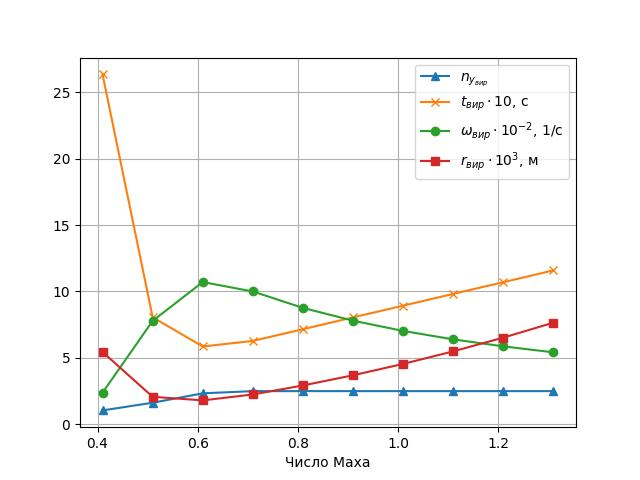
\includegraphics[width=\linewidth]{Оглавление/Part1/figures/РезультатыМаневры.jpg}}
    \caption{Характеристики правильного предельного виража }
    \label{fig:image}
\end{figure}

\begin{figure}[H]
    \center{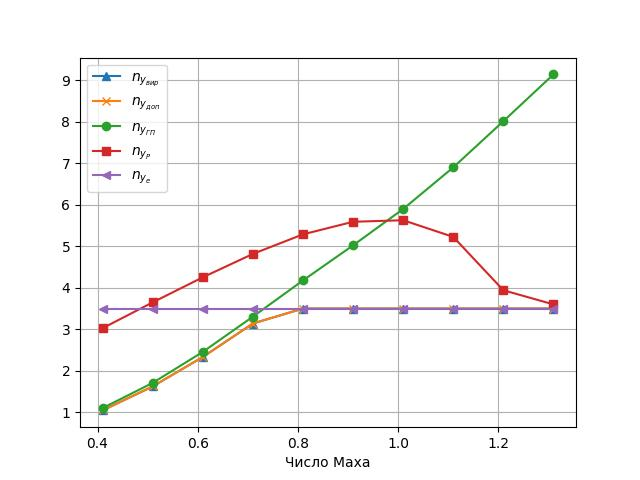
\includegraphics[width=\linewidth]{Оглавление/Part1/figures/РезультатыМаневры2.jpg}}
    \caption{Перегрузки при выполнении виража}
    \label{fig:image}
\end{figure}

\begin{center}
    Выводы:
\end{center}

В ходе расчетов в данном разделе были получены следующие результаты:
\begin{itemize}
    \item [-] угловая скорость виража изменяется от 0,024 $\frac{1}{c}$ до 0,08 $\frac{1}{c}$ на диапазоне
чисел М, при которых возможен правильный предельный вираж на высоте 6 км
    \item [-] радиус виража изменяется в диапазоне от 5443,8 м до 5227,8 м
    \item [-] время выполнения виража изменяется в диапазоне от 263,3 с до 79,2 с
\end{itemize}
По полученным данным можно сказать, что самолет –прототип Concorde обладает
довольно хорошими характеристиками предельного правильного виража






% \subsection{Расчёт характеристик продольной устойчивости самолёта}
\label{sec:Расчёт характеристик продольной устойчивости самолёта}
\pagestyle{fancy}
\fancyhf{}
\rhead{Дипломная работа}
\lhead{Расчёт траектории полёта}
\rfoot{\thepage}



Прежде чем приступить к расчету характеристик продольной статической устойчивости и управляемости необходимо определить безразмерную площадь горизонтальногооперения $\bar{S}_\text{ГО}$ из условия устойчивости и балансировки.

Далее вычисляется следующие характеристики:
\begin{enumerate}
    \item Зависимости от числа М (скорости) полета:
    \begin{itemize}
        \item [-] запаса статической устойчивости по перегрузке $\sigma_n$,
        \item [-] фокуса самолета $\bar{X}_F$,
        \item [-] точки нейтральности по перегрузке $\bar{X}_H$,
        \item [-] предельно задней центровки $\bar{X}_\text{ТПЗ}$.
    \end{itemize}
    \item Зависимость от числа М (скорости) полета:
    \begin{itemize}
        \item [-] балансировочного отклонения органа продольного управления $\varphi_\text{бал}(\delta_\text{бал})$,
        \item [-] градиента отклонения органа продольного управления по перегрузки
        \item [-] располагаемой нормальной перегрузки из условия балансировки.
    \end{itemize}
\end{enumerate}

Для определения площади ГО ($S_\text{ГО}$) рассчитываются предельно передняя $\bar{X}_\text{ТПП}$ и предельного значения $\bar{X}_\text{ТПЗ}$ центровки.Расчёт предельно передней центровки ведётся для режима пасадки ($H = 0$ км, $M = 0,2$). Предельно передняя центровка вычисляется для указанного режима вычисляется по формуле

\begin{equation}
    \label{eq:Предельно передняя центровка}
    \bar{X}_\text{ТПП} = \frac{-m_{z_0 \text{БГО}} + \bar{X}_{F \ \text{БГО}}  \cdot  C_{y \ \text{БГО}} + C_{y \ \text{ГО}} \cdot \bar{S}_\text{ГО} \cdot K_\text{ГО} \cdot \bar{L}_\text{ГО}}{C_{y \ \text{БГО}}}
\end{equation}

\begin{equation}
    \label{eq:CyБГО}
    C_{y \ \text{БГО}} = C_{y_0 \ \text{БГО}} + C_{y \text{БГО}}^\alpha \cdot \alpha
\end{equation}  

\begin{equation}
    \label{eq:CyГО}
    C_{y \ \text{ГО}} = C_{y \ \text{ГО}}^{\alpha_\text{ГО}}[\alpha(1 - \varepsilon^\alpha) + \varphi_\text{ЭФ}] < 0
\end{equation}

\begin{equation}
    \label{eq:fiЭФ}
    \varphi_\text{ЭФ} = \varphi_\text{уст} + n_B \cdot \delta_{max}
\end{equation}

Аэродинамические характеристики самолета без ГО и ВО для режима посадки указаны в исходных данных.

Величина угла атаки при посадке (касании ВПП) приведена в разделе \ref{sec:Расчет взлетно-посадочных характеристик самолета}. Предельно задняя центровка вычисляется для режима $H=0$ км, $M=0,3$ по формуле

\begin{equation}
    \label{eq:Предельно задняя центровка}
    \bar{X}_\text{ТПЗ} = \bar{X}_\text{Н} + \sigma_{n \ min}
\end{equation}

\begin{equation}
    \label{eq:Нейтральная центровка}
    \bar{X}_H = \bar{X}_F - \frac{m_z^{\bar{\omega}_z}}{\mu}
\end{equation}

\begin{equation}
    \label{eq:Относительная плотность самолёта}
    \mu = 2\frac{P_s}{\rho g b_a}
\end{equation}

\begin{equation}
    \label{eq:Относительный коэффициент демпфирующего момента}
    m_z^{\bar{\omega}_z} = m_z^{\bar{\omega}_{z \ \text{БГО}}} + m_z^{\bar{\omega}_{z \ \text{ГО}}}
\end{equation}

\begin{equation}
    \label{eq:bar(wz)ГО}
    m_z^{\bar{\omega}_z}_{\text{ГО}} = -C_{y \ \text{ГО}}^{\alpha_\text{ГО}} \bar{S}_\text{ГО} \bar{L}_\text{ГО} \sqrt{K_\text{ГО}}
\end{equation}

\begin{equation}
    \label{eq:Относительная координата фокуса}
    \bar{X}_F = \bar{X}_{F \ \text{БГО}} + \Delta \bar{X}_F
\end{equation}

\begin{equation}
    \label{eq:Изменение относительной координаты фокуса}
    \Delta \bar{X}_F \approx \frac{C_{y \ \text{ГО}}^{\alpha_\text{ГО}}}{C_y^\alpha} (1 - \varepsilon^\alpha) \bar{S}_\text{ГО} \bar{L}_\text{ГО} K_\text{ГО}
\end{equation}

$\sigma_{n_{min}} = 0,1 $,  для неманёвренных самолётов

По приведенным выше формулам \ref{eq:Предельно передняя центровка} - \ref{eq:Изменение относительной координаты фокуса} для ряда значений $S_\text{ГО}$ (0.05,0.2) были рассчитаны предельно передняя и предельно задняя центровки.

\begin{center}
    Расчёт $\bar{S}_\text{ГО}$:
\end{center}

\begin{table}[H]
    \centering
        \caption{Предельная задняя и предельная передняя центровки }
    \begin{tabular}{|c|c|c|}
        \hline
        $\bar{S}_\text{ГО}$ & 0,05 & 0,2\\ \hline
        $\bar{X}_\text{ТПП}$ &  & \\ \hline
        $\bar{X}_\text{ТПЗ}$ &  & \\ \hline
    \end{tabular}
    \label{tab:Предельная задняя и предельная передняя центровки}
\end{table}

Затем на одном рисунке строятся зависимости $\bar{X}_\text{ТПП}(\bar{S}_\text{ГО})$, $\bar{X}_\text{ТПЗ}(\bar{S}_\text{ГО})$ графически определяется потребная площадь ГО(см. рис.\ref{fig:Нахождение S_ГО}) из условия: $\bar{X}_\text{ТПЗ}(\bar{S}_\text{ГО}) -\bar{X}_\text{ТПП}(\bar{S}_\text{ГО}) = \Delta \bar{X}_\text{э} \cdot 1,2$, где $\Delta \bar{X}_\text{э}$ -- эксплуатационный разброс центровок 
$\Delta \bar{X}_\text{э} \approx 0,15$ -- для неманёвренных самолётов.

\begin{figure}[H]
    \center{\includegraphics[width=\linewidth]{.jpg}}
    \caption{Нахождение $\bar{X}^*_\text{ГО}$}
    \label{fig:Нахождение S_ГО}
\end{figure}

Далее расчеты характеристик устойчивости и управляемости производятся для
средней центровки: 

\begin{equation}
    \label{eq:Средняя центровка}
    \bar{X}_T = \frac{1}{2} [\bar{X}_\text{ТПЗ}(\bar{S}^*_\text{ГО}) +\bar{X}_\text{ТПП}(\bar{S}^*_\text{ГО})]
\end{equation}
$\bar{S}_\text{ГО}^* = $

Используя ранее приведённые уравнения получим:

$\bar{X}_T = $

При расчете зависимостей $\bar{X}_T(M)$, $\bar{X}_H(M)$, $\bar{X}_\text{ТПЗ}$ используются
формулы \ref{eq:Предельно передняя центровка} - \ref{eq:Изменение относительной координаты фокуса} 

Величина $\sigma_n$ определяется выражением 
\begin{equation}
    \label{eq:Коэффициент продольной статической устойчивости по перегрузке}
    \sigma_n = \bar{X}_T - \bar{X}_F + \frac{m_z^{\bar{\omega}_z}}{\mu}
\end{equation}

Значения величин $\bar{X}_T$, $\bar{X}_F$, $\bar{X}_\text{ТПЗ}$,  $\sigma_n$ определяются в узловых точках $M$ на высоте $H = 0$ км. Результаты данного расчёта оформлены в виде таблицы \ref{tab:Результаты расчётов балансировки в продольном канале}  

\begin{figure}[H]
    \center{\includegraphics[width=\linewidth]{.jpg}}
    \caption{Представление результатов расчета в виде графиков}
    \label{fig:Результаты расчётов балансировки в продольном канале}
\end{figure}

Зависимости $\varphi_\text{бал}(M)[\delta_\text{бал}(V)]$, $\varphi^n(M)[\delta^n(V)]$, $n_{y_P}(M)[n_{y_P}(V)]$ определяютс для трёх значений: $H = 0$ км, $H = 6$ км и высоты крейсерского полёта $H_\text{кр}$, найденных в разделе \ref{sec:Расчет летно-технических характеристик самолета} 
\begin{center}
    Вычисление балансировочного значения руля высоты:
\end{center}

\begin{equation}
    \label{eq:Балансировочное значение руля высоты}
    \delta_\text{бал} = -\frac{m_{x_0}+m^{C_{y \ \text{ГП}}}_{z_{C_{y \ \text{ГП}}}}}{m_z^\delta(1 + \frac{m_z^{C_y}}{\bar{L}_\text{ГО}})}-\frac{\varphi_\text{уст}}{n_\text{В}}
\end{equation}

$$\bar{m} = 1 - \bar{m}_T - \text{относительная масса самолёта}$$

\begin{equation}
    \label{eq:ГП балансировка}
    C_{y_\text{ГП}} = \frac{P_s \cdot \bar{m}}{q}
\end{equation}

\begin{equation}
    \label{eq:mzCy}
    m_z^{C_y} = \bar{X}_T - \bar{X}_F
\end{equation}

\begin{equation}
    \label{eq:Расход руля высоты}
    n_B = \frac{C_y^\delta}{C_y^\varphi}
\end{equation}

\begin{equation}
    \label{eq:Балансировочное значение коэффициента нулевого продольного момента}
    m_{z_0} = m_{z_{0 \ \text{БГО}}} - \bar{S}_\text{ГО} \bar{L}_\text{ГО} K_\text{ГО} C^{\alpha_\text{ГО}}_{y_\text{ГО}} \alpha_0(1 - \varepsilon^\alpha)
\end{equation}

\begin{center}
    Вычисление отклонения стабилизатора на единицу перегрузки:
\end{center}

\begin{equation}
    \label{eq:delta_n}
    \delta^n = -\frac{C_{y_\text{ГП}} \cdot \sigma_n}{m_z^\delta}
\end{equation}

\begin{equation}
    \label{eq:mzdelta}
    m_z^\delta = -C^{\alpha_\text{ГП}}_{y_\text{ГП}} \bat{S}_\text{ГП} \bar{L}_\text{ГП} K_\text{ГП} n_B
\end{equation}

\begin{center}
    Вычисление отклонения стабилизатора на единицу перегрузки:
\end{center}

\begin{equation}
    \label{eq:Располагаемая перегрузка}
    n_{y_\text{Р}} = 1 + \frac{(\delta_{max}) - (\delta_\text{бал})}{\delta^n}
\end{equation}

Результаты расчетов оформлены в виде таблиц \ref{tab:} - \ref{tab:}




\newpage
\section{Синтез системы автоматического управления}

\subsection{Общие положения}

\textit{Цель раздела} -- расчет коэффициентов и моделирование системы стабилизации вертикальной скорости самолета для Concorde: выбор параметров привода, расчет и оценка коэффициентов обратных связей и коэффициентов стабилизации системы, частотный анализ контуров системы, моделирование и анализ линейной и нелинейной САУ. 


\subsection{Составление математической модели}

Для того, чтобы подобрать коэффициенты обратных связей необходимо сначала составить схему системы стабилизации вертикальной скорости самолета, далее проанализировав схему, определиться со способами нахождения рациональных значений коэффициентов. Для начала запишем уравнения продольного движения самолета (формула \ref{eq:СДУ}):

\begin{equation}
    \label{eq:СДУ}
    \begin{cases}
        \dot{\sin{\alpha}}=\omega_z-\omega_x \sin{\beta}-\bar{Y}^{\alpha} \alpha \\
        \dot{\omega}_z=-A \omega_x \omega_y+\bar{M}_z^{\alpha} \alpha+\bar{M}_z^{\omega_z} \omega_z +\bar{M}_z^{\dot{\alpha}} \dot{\alpha}+\bar{M}_z^{\delta_{\text{в}}} \delta_{\text{в}} \\
        \dot{H}=V\sin{\theta}
    \end{cases}
\end{equation}

Для системы (\ref{eq:СДУ}) примем ряд следующих допущений:
\begin{enumerate}
    \item Так как работа системы стабилизации будет производиться с $\beta=0$, то $\sin{\beta}=0$ => взаимодействие продольного и бокового движения незначительно.
    \item Угол наклона траектории меняется незначительно => $\sin{\theta} \approx \theta$.
    \item Считаем, что угл атаки меняется в небольшом диапозоне $\sin{\alpha} \approx \alpha$, а $\cos{\alpha} \approx 1$
\end{enumerate}

Введя данные допущения, получаем следующую систему дифференциальных уравнений (\ref{eq:Упрощённая СДУ})

\begin{equation}
    \label{eq:Упрощённая СДУ}
    \begin{cases}
        \dot{\alpha}=\omega_z-\bar{Y}^{\alpha} \alpha \\
        \dot{\omega}_z=\bar{M}_z^{\alpha} \alpha+\bar{M}_z^{\omega_z} \omega_z +\bar{M}_z^{\dot{\alpha}} \dot{\alpha}+\bar{M}_z^{\delta_{\text{в}}} \delta_{\text{в}} \\
        \dot{V_y}=V \cdot \bar{Y}^{\alpha} \alpha
    \end{cases}
\end{equation}

Преобразуем дифференциальное уравнение $\dot{H}=V\sin{\theta}$ 
$$\dot{H}=V\sin{\theta} \approx V \cdot \theta $$
$$\theta = \vartheta - \alpha$$
$$\dot{H}=V(\vartheta - \alpha)$$
$$\dot{V}_y =\ddot{H}=V(\omega_z - \dot{\alpha})=V(\omega_z-\omega_z+\bar{Y}^{\alpha} \alpha)=V \cdot \bar{Y}^{\alpha} \alpha$$
\begin{equation}
    \dot{V_y}=V \cdot \bar{Y}^{\alpha} \alpha
\end{equation}

Из системы уравнений (\ref{eq:Упрощённая СДУ}), применив преобразование Лапласа можно получить следующие передаточные функции:

\begin{equation}
    \label{eq:ПФ угл атаки}
   \left \{ \frac{\alpha}{\delta_\text{э}} \right \}
    =\frac{\bar{M}_z^{\delta_{\text{в}}}}{p^2+2hp+\omega_0^2}
\end{equation}
\begin{equation}
    \label{eq:ПФ угловой скорости тангажа}
   \left \{ \frac{\omega_z}{\delta_\text{э}} \right \}
    =\frac{\bar{M}_z^{\delta_{\text{э}}}(p+\bar{Y}^{\alpha})}{p^2+2hp+\omega_0^2}
\end{equation}
\begin{equation}
    \label{eq:ПФ угл тангажа}
    \left \{ \frac{\vartheta}{\delta_\text{э}} \right \}=\frac{1}{p} \cdot \left \{ \frac{\omega_z}{\delta_\text{э}} \right \}=\frac{\bar{M}_z^{\delta_{\text{э}}}(p+\bar{Y}^{\alpha})}{ p (p^2+2hp+\omega_0^2)}
\end{equation}
\begin{equation}
    \label{eq:ПФ вертикальная скорость}
   \left \{ \frac{V_y}{\delta_\text{э}} \right \}
    = \frac{V \cdot \bar{Y}^{\alpha}\bar{M}_z^{\delta_{\text{э}}}}{p^2+2hp+\omega_0^2}
\end{equation}

\begin{equation}
    \label{eq:ПФ вертикальной скорости по углу тангажа}
   \left \{ \frac{V_y}{\vartheta} \right \}
    = \frac{\bar{Y}^{\alpha}}{p+\bar{Y}^{\alpha}}K_H =  \frac{K_H}{T_1_c p+1}
\end{equation}

Так как в двнной работе в основном используется моделирование динамической системы через \textit{State space}, запишем для него матрицы пространств состояний:
$$A = \begin{pmatrix}
-\bat{Y^{\alpha}} & 1 & 0\\ 
\bar{M}_z^\alpha & \bar{M}_z^{\omega_z} & 0\\ 
 V \cdot \bar{Y}^\alpha& 0 & 0 
\end{pmatrix}$$

$$B = \begin{pmatrix}
 0 \\ 
 \bar{M}_z^{\delta_{\text{э}}} \\ 
 0 
\end{pmatrix}$$

$$C= \begin{pmatrix}
1 & 0 & 0\\ 
0 & 1 & 0\\ 
 0& 0 &1 
\end{pmatrix}$$

$$D = \begin{pmatrix}
 0 \\ 
 0 \\ 
 0 
\end{pmatrix}$$

Зная вышеприведенные матрицы пространств состояний, можно составить следующую схему стабилизации вертикальной скорости самолёта (см.рис.\ref{fig:Схема}).


\begin{figure}[H]
    \center{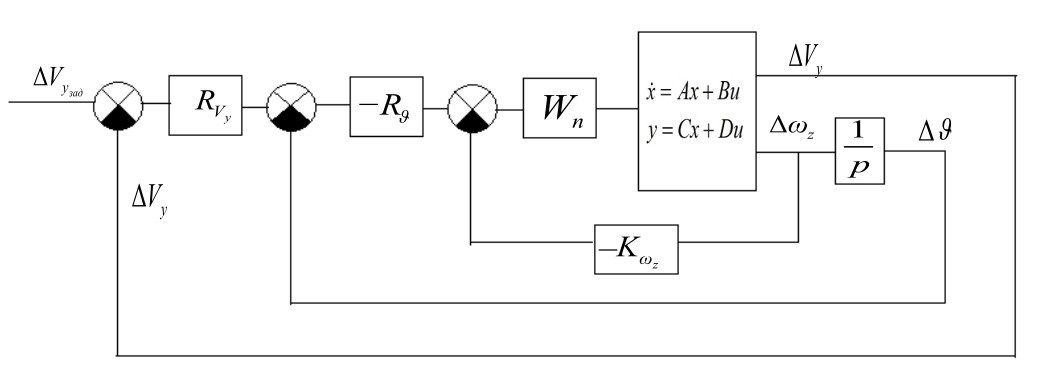
\includegraphics[width=\linewidth]{Оглавление/Part2/Sactions/Content/figures/Схема.jpg}}
    \caption{Структурная схема системы стабилизации вертикальной скорости самолета}
    \label{fig:Схема}
\end{figure}

\subsection{Выбор параметров привода}
    
    При решении задачи синтеза сервопривод описывается передаточной функций колебательного звена:
    
    \begin{equation}
    \label{eq:Привод ограничеия}
        W_{\text{п}}=\frac{1}{T_\text{п}^2p^2+2\xi_\text{п}T_\text{п}p+1}
    \end{equation}
    
    Значение постоянной времени  $T_\text{п}$ сервопривода, от которой зависит его полоса пропускания, определяется следующим образом:
    
    Устанавливается максимальное значение собственной частоты  недемпфированных колебаний $\omega_0=\frac{1}{T_{\text{с}}}$ в варианте управлении продольным движением самолета, и исходя из этих значений, определяется потребная ширина полосы пропускания сервопривода (см. формула \ref{eq:Привод ограничеия}):
    
    \begin{equation}
        \label{eq:Собственная частота привода}
        \omega_\text{п}=10 \omega_{0_{max}}
    \end{equation}
    
    По найденному значению $\omega_\text{п}$ определяется постоянная времени  $T_\text{п}$ как ближайшее к величине $1/ \omega_\text{п}$  значение из ряда чисел: [0,02; 0,025; 0,003; 0,035; 0,04; 0,045; 0,05] (в данном ряде чисел указаны значения постоянной времени, характерные для современных сервоприводов).
    
    \subsubsection{Расчёт $\omega_0$}
    
    Относительный момент тангажа по углу атаки -- 
    \begin{equation}
        \label{eq:Относительный момент тангажа по углу атаки}
        \bar{M}_z^{\alpha} = \frac{m_z^{\alpha}qSb_a}{J_z}
    \end{equation}
    
    Относительная производная подъёмной силы по углу атаки --
    \begin{equation}
        \label{eq:Относительный момент тангажа по угловой скорости тангажа}
        \bar{Y}^\alpha=\frac{C_y^\alpha qS}{mV}
    \end{equation}
    
    Относительный демпфирующий момент тангажа --
    \begin{equation}
        \label{eq:Относительный демпфирующий момент тангажа}
        \bar{M}^{\omega_z}=\frac{m_z^{\omega_z} qS b_a}{J_z}
    \end{equation}
    
    
    Квадрат частоты собственных недемпфированных колебаний --
    \begin{equation}
        \label{eq:Cобственная частота самолёта}
        \omega_0^2=-\bar{Y}^\alpha \bar{M}_z^{\omega_z}-\bar{M}_z^{\alpha}
    \end{equation}
    
    Согласно формулам \ref{eq:Относительный момент тангажа по углу атаки}-\ref{eq:Cобственная частота самолёта} были произведены все необходимые вычисления для каждой узловой точки, результаты вычислений занесены в таблицы \ref{tab:Узловые точки}-\ref{tab:Собственные значения частоты недемпфированных колебаний в узловых точках}


  \begin{longtable}[H]{|c|c|c|c|c|c|c|c|c|c|c|}
    \caption{$\omega_0$ в узловых точках (таб. \ref{tab:Узловые точки})\label{tab:Собственные значения частоты недемпфированных колебаний в узловых точках}}
    \hline 
    $H,$ км &\multicolumn{10}{|c|}{$\omega_0, 1/c$} \\ \hline
    \endfirsthead
    
    \multicolumn{11}{c}%
    {{ \tablename\ \thetable{}: $\omega_0$ в узловых точках}} \\
    \hline 
    $H,$ км &\multicolumn{10}{|c|}{$\omega_0, 1/c$} \\ \hline
    \endhead
    \endfoot
    
    \hline \hline
    \endlastfoot

    0 & 0,88 & 1,21 & 1,54 & 1,87 & 2,24 & 2,64 & 3,13 & 3,78 & 4,66 & 5,74  \\ \hline
    1 & 0,86 & 1,16 & 1,47 & 1,78 & 2,12 & 2,51 & 2,99 & 3,65 & 4,53 & 5,59  \\ \hline
    2 & 0,84 & 1,12 & 1,39 & 1,69 & 2,01 & 2,37 & 2,86 & 3,53 & 4,4 & 5,44  \\ \hline
    3 & 0,81 & 1,07 & 1,32 & 1,6 & 1,9 & 2,25 & 2,74 & 3,41 & 4,28 & 5,3  \\ \hline
    4 & 0,79 & 1,02 & 1,25 & 1,51 & 1,79 & 2,14 & 2,63 & 3,31 & 4,16 & 5,15  \\ \hline
    5 & 0,77 & 0,98 & 1,2 & 1,44 & 1,71 & 2,06 & 2,56 & 3,24 & 4,07 & 5,01  \\ \hline
    6 & 0,75 & 0,94 & 1,15 & 1,37 & 1,63 & 1,98 & 2,49 & 3,17 & 3,98 & 4,87  \\ \hline
    7 & 0,73 & 0,91 & 1,09 & 1,3 & 1,56 & 1,92 & 2,44 & 3,11 & 3,89 & 4,72  \\ \hline
    8 & 0,7 & 0,87 & 1,04 & 1,24 & 1,49 & 1,86 & 2,39 & 3,04 & 3,79 & 4,55  \\ \hline
    9 & 0,69 & 0,84 & 1 & 1,19 & 1,45 & 1,82 & 2,33 & 2,95 & 3,64 & 4,32  \\ \hline
    10 & 0,68 & 0,82 & 0,97 & 1,15 & 1,41 & 1,78 & 2,27 & 2,85 & 3,48 & 4,08  \\ \hline
    11 & 0,67 & 0,79 & 0,93 & 1,11 & 1,37 & 1,75 & 2,22 & 2,75 & 3,32 & 3,85  \\ \hline
    12 & 0,65 & 0,76 & 0,9 & 1,08 & 1,35 & 1,71 & 2,15 & 2,65 & 3,16 & 3,62  \\ \hline
    13 & 0,65 & 0,76 & 0,89 & 1,07 & 1,33 & 1,66 & 2,05 & 2,47 & 2,9 & 3,29  \\ \hline
    14 & 0,66 & 0,76 & 0,9 & 1,08 & 1,33 & 1,62 & 1,95 & 2,3 & 2,66 & 2,99  \\ \hline
    15 & 0,68 & 0,78 & 0,92 & 1,1 & 1,32 & 1,57 & 1,85 & 2,15 & 2,45 & 2,72  \\ \hline
    16 & 0,71 & 0,81 & 0,95 & 1,12 & 1,32 & 1,53 & 1,76 & 2,01 & 2,25 & 2,48  \\ \hline
    17 & 0,82 & 0,92 & 1,04 & 1,16 & 1,3 & 1,45 & 1,6 & 1,76 & 1,92 & 2,08  \\ \hline
    18 & 0,98 & 1,05 & 1,13 & 1,21 & 1,29 & 1,37 & 1,45 & 1,54 & 1,63 & 1,72  \\ \hline
    19  & 1,17 & 1,19 & 1,22 & 1,24 & 1,27 & 1,29 & 1,32 & 1,35 & 1,37 & 1,4 \\ \hline
    \end{longtable}

По данным таблицы \ref{tab:Собственные значения частоты недемпфированных колебаний в узловых точках} можно сделать вывод, что максимальное значение $\omega_0$ находится у поверхности земли со значением $M = 1$ ($\omega_0_{max} = 3.719 \ \frac{1}{c}$).

Используя соотношение (\ref{eq:Собственная частота привода}) получаем, что $\omega_\text{п} = 37,19 \ \frac{1}{c}$ => $T_{\text{п}} = 0.0269 \ c$ 

Из данного ряда чисел [0,02; 0,025; 0,003; 0,035; 0,04; 0,045; 0,05] 0,0269 более близко к 0,025, следовательно, данное число мы и примем за постоянную времени привода. Исходя из вышесказанного, получаем $\omega_\text{п} = 40 \ \frac{1}{c}$ , $T_{\text{п}} = 0.025 \ c, \xi = 0,5$.


    $$W_{\text{п}} = \frac{1}{T_{\text{п}}^2p^2+2\xi_\text{п}T_{\text{п}}p+1} = \frac{1}{0,000156252p^2+0,0125p+1}$$
    
    \begin{center}
        Выводы:
    \end{center}
    
    После выполнения необходимых расчетов преобразований были найдены следующие параметры привода системы стабилизации вертикальной скорости:\\
    $\omega_\text{п} = 40 \ \frac{1}{c}$ \\
    $T_{\text{п}} = 0.025 \ c \\
    \xi = 0,5$\\
    
    Найденные значения параметров соответствуют стандартным значениям для параметров привода и могут быть использованы в последующих частях данной работы. 

    \subsection{Синтез контуров автоматического управления}
    \subsubsection{Выбор коэффициентов обратных связей}
    
    После определения  параметров привода необходимо выбрать рациональные значения коэффициентов обратных связей. Для начала необходимо подобрать коэффициенты $K_\omega_z$ и $K_\vartheta$.
    
    % \subsubsection{Методика расчёта $K_{\vartheta}$}
    
    \subsubsubsection{Методика расчёта  $K_{\omega_z}$ и $K_\vartheta$}
    
    Составим передаточную функцию разомкнутого контура стабилизации угла тангажа
    
    \begin{equation}
    \label{eq:ПФ разомкнутой системы стабилизации тангажа}
        W_{\text{раз} \ \vartheta} = \frac{\Mzf K_{\omega_z}(p+\nu)(T_1_c p+1)}{p(p^2 +2hp+\omega_0^2)(T_{\text{п}}^2p^2+2\xi_\text{п}T_{\text{п}}p+1)},
    \end{equation}
    где $\nu=\frac{K_\vartheta}{K_{\omega_z}}$

    Если выбрано $\nu \approx \frac{1}{T_c}=\omega_0$, то асимптотическая ЛАФЧХ прередаточной функции (\ref{eq:ПФ разомкнутой системы стабилизации тангажа}) имеет 2 участка с наклоном -20 дБ/дек: первый при $\omega < \frac{1}{T_1_c}$, второй  -- при $\frac{1}{T_c}<\omega<\frac{1}{T_\text{п}}$. Для интересующей нас второй асимптоты ЛАФЧХ с наклоном -20 дБ/дек на основе (\ref{eq:ПФ разомкнутой системы стабилизации тангажа}) получим следующую формулу:
    
    \begin{equation}
    \label{eq:ПФ разомкнутой системы стабилизации тангажа 2}
        W_{\text{раз} \ \vartheta} = \frac{K_{\omega_z} T_1_c}{T_c^2p}=-\frac{K_{\omega_z} \Mzf}{p}, \frac{1}{T_c} < \omega < \frac{1}{T_{\text{п}}}.
    \end{equation}
    
    Частота среза частотной характеристики передаточной функции (\ref{eq:ПФ разомкнутой системы стабилизации тангажа 2}) $\omega_{cp} = K_{\omega_z}\Mzf.$ Так как фазовая частотная характеристика передаточной функции (\ref{eq:ПФ разомкнутой системы стабилизации тангажа}) достигает значения $-\pi$ на частоте $\omega_{-\pi} \approx \frac{1}{T_\text{п}}$, то для граничного значения $K_{\omega_z}$ (при котором $\omega_{cp} = \omega_{-\pi}$) имеем 
    
    \begin{equation}
        K_{\omega_z_{\text{гр}}} = \frac{1}{|\Mzf|T_\text{п}}.
    \end{equation}
    
    Исходя из запаса по амплитуде 12 дБ/дек можно принять 
    \begin{equation}
        \label{eq:K_wz}
        K_{\omega_z} = 0,25K_{\omega_z_{\text{гр}}}, \ \ \frac{K_{\vartheta}}{K_{\omega_z}} < \frac{0,25}{T_\text{п}}.
    \end{equation}

    \subsubsubsection{Результаты расчётов $K_{\omega_z}$ и $K_\vartheta$}
    
    \begin{longtable}[H]{|c|c|c|c|c|c|c|c|c|c|c|}
    \caption{Результаты расчётов $K_{\omega_z}, c$ в узловых точках (таб. \ref{tab:Узловые точки})}
    \hline 
    $H,$ км &\multicolumn{10}{|c|}{$K_{\omega_z}, c$} \\ \hline
    \endfirsthead
    
    \multicolumn{11}{c}%
    {{ \tablename\ \thetable{}: Результаты расчётов $K_{\omega_z}, c$ в узловых точках}} \\
    \hline 
    $H,$ км &\multicolumn{10}{|c|}{$K_{\omega_z}, c$} \\ \hline
    \endhead
    \endfoot
    
    \hline \hline
    \endlastfoot

    \hline
    0 & 6,11 & 3,24 & 1,98 & 1,3 & 0,9 & 0,67 & 0,51 & 0,36 & 0,23 & 0,15  \\ \hline
    1 & 6,01 & 3,29 & 2,04 & 1,35 & 0,95 & 0,71 & 0,53 & 0,37 & 0,23 & 0,15  \\ \hline
    2 & 5,98 & 3,37 & 2,12 & 1,41 & 1 & 0,76 & 0,56 & 0,38 & 0,24 & 0,16  \\ \hline
    3 & 6,02 & 3,47 & 2,21 & 1,49 & 1,07 & 0,81 & 0,59 & 0,39 & 0,25 & 0,17  \\ \hline
    4 & 6,11 & 3,6 & 2,31 & 1,57 & 1,15 & 0,87 & 0,62 & 0,4 & 0,25 & 0,17  \\ \hline
    5 & 6 & 3,64 & 2,37 & 1,64 & 1,22 & 0,91 & 0,63 & 0,4 & 0,26 & 0,18  \\ \hline
    6 & 5,98 & 3,71 & 2,46 & 1,73 & 1,3 & 0,96 & 0,65 & 0,41 & 0,27 & 0,19  \\ \hline
    7 & 6,01 & 3,81 & 2,56 & 1,83 & 1,39 & 1,01 & 0,66 & 0,42 & 0,28 & 0,21  \\ \hline
    8 & 6,11 & 3,94 & 2,69 & 1,96 & 1,49 & 1,06 & 0,68 & 0,43 & 0,3 & 0,22  \\ \hline
    9 & 5,93 & 3,94 & 2,77 & 2,08 & 1,57 & 1,09 & 0,7 & 0,46 & 0,32 & 0,25  \\ \hline
    10 & 5,82 & 3,99 & 2,9 & 2,22 & 1,66 & 1,13 & 0,73 & 0,49 & 0,35 & 0,28  \\ \hline
    11 & 5,79 & 4,09 & 3,07 & 2,37 & 1,74 & 1,16 & 0,76 & 0,53 & 0,39 & 0,31  \\ \hline
    12 & 5,82 & 4,24 & 3,27 & 2,52 & 1,81 & 1,2 & 0,81 & 0,57 & 0,43 & 0,35  \\ \hline
    13 & 5,44 & 4,22 & 3,36 & 2,59 & 1,85 & 1,27 & 0,89 & 0,65 & 0,51 & 0,42  \\ \hline
    14 & 5,23 & 4,26 & 3,42 & 2,62 & 1,89 & 1,34 & 0,98 & 0,75 & 0,6 & 0,5  \\ \hline
    15 & 5,15 & 4,26 & 3,42 & 2,6 & 1,92 & 1,42 & 1,08 & 0,86 & 0,7 & 0,6  \\ \hline
    16 & 5,05 & 4,17 & 3,32 & 2,55 & 1,95 & 1,51 & 1,2 & 0,98 & 0,82 & 0,71  \\ \hline
    17 & 4,27 & 3,58 & 2,96 & 2,44 & 2,02 & 1,69 & 1,44 & 1,24 & 1,08 & 0,96  \\ \hline
    18 & 3,3 & 2,94 & 2,62 & 2,35 & 2,11 & 1,9 & 1,72 & 1,57 & 1,44 & 1,33  \\ \hline
    19  & 2,53 & 2,44 & 2,36 & 2,28 & 2,2 & 2,13 & 2,06 & 2 & 1,94 & 1,88 \\ \hline
    \end{longtable}

    \begin{longtable}[H]{|c|c|c|c|c|c|c|c|c|c|c|}
    \caption{Результаты расчётов $K_{\vartheta}$ в узловых точках (таб. \ref{tab:Узловые точки})}
    \hline 
    $H,$ км &\multicolumn{10}{|c|}{$K_{\vartheta}$ } \\ \hline
    \endfirsthead
    
    \multicolumn{11}{c}%
    {{ \tablename\ \thetable{}: Результаты расчётов $K_{\vartheta}$ в узловых точках}} \\
    \hline 
    $H,$ км &\multicolumn{10}{|c|}{$K_{\vartheta}$ } \\ \hline
    \endhead
    \endfoot
    
    \hline \hline
    \endlastfoot

    0 & 2,82 & 1,79 & 1,29 & 0,97 & 0,76 & 0,63 & 0,53 & 0,41 & 0,29 & 0,21  \\ \hline
    1 & 2,71 & 1,75 & 1,27 & 0,96 & 0,76 & 0,63 & 0,52 & 0,4 & 0,28 & 0,21  \\ \hline
    2 & 2,58 & 1,72 & 1,25 & 0,95 & 0,75 & 0,63 & 0,51 & 0,38 & 0,27 & 0,2  \\ \hline
    3 & 2,54 & 1,71 & 1,24 & 0,94 & 0,76 & 0,63 & 0,5 & 0,36 & 0,26 & 0,2  \\ \hline
    4 & 2,51 & 1,7 & 1,23 & 0,95 & 0,76 & 0,63 & 0,49 & 0,35 & 0,25 & 0,19  \\ \hline
    5 & 2,41 & 1,64 & 1,21 & 0,94 & 0,77 & 0,62 & 0,48 & 0,33 & 0,24 & 0,19  \\ \hline
    6 & 2,34 & 1,64 & 1,21 & 0,93 & 0,77 & 0,62 & 0,45 & 0,32 & 0,23 & 0,19  \\ \hline
    7 & 2,29 & 1,6 & 1,18 & 0,94 & 0,77 & 0,61 & 0,43 & 0,3 & 0,23 & 0,19  \\ \hline
    8 & 2,21 & 1,58 & 1,19 & 0,95 & 0,78 & 0,59 & 0,41 & 0,29 & 0,22 & 0,19  \\ \hline
    9 & 2,14 & 1,54 & 1,17 & 0,96 & 0,77 & 0,58 & 0,4 & 0,29 & 0,23 & 0,19  \\ \hline
    10 & 2,04 & 1,48 & 1,16 & 0,96 & 0,77 & 0,55 & 0,39 & 0,29 & 0,23 & 0,2  \\ \hline
    11 & 1,98 & 1,48 & 1,2 & 0,98 & 0,75 & 0,54 & 0,38 & 0,29 & 0,24 & 0,21  \\ \hline
    12 & 1,87 & 1,45 & 1,18 & 0,99 & 0,74 & 0,52 & 0,37 & 0,29 & 0,24 & 0,21  \\ \hline
    13 & 1,75 & 1,4 & 1,18 & 0,96 & 0,71 & 0,51 & 0,38 & 0,3 & 0,26 & 0,23  \\ \hline
    14 & 1,63 & 1,37 & 1,13 & 0,92 & 0,68 & 0,51 & 0,39 & 0,32 & 0,28 & 0,25  \\ \hline
    15 & 1,55 & 1,33 & 1,1 & 0,86 & 0,66 & 0,51 & 0,4 & 0,34 & 0,3 & 0,26  \\ \hline
    16 & 1,47 & 1,26 & 1,03 & 0,82 & 0,65 & 0,52 & 0,42 & 0,36 & 0,31 & 0,29  \\ \hline
    17 & 1,24 & 1,04 & 0,89 & 0,76 & 0,63 & 0,54 & 0,48 & 0,42 & 0,38 & 0,35  \\ \hline
    18 & 0,96 & 0,86 & 0,76 & 0,68 & 0,63 & 0,57 & 0,54 & 0,49 & 0,46 & 0,43  \\ \hline
    19  & 0,71 & 0,69 & 0,66 & 0,66 & 0,64 & 0,62 & 0,6 & 0,58 & 0,56 & 0,55 \\ \hline
    \end{longtable}
 
    \begin{longtable}[H]{|c|c|c|c|c|c|c|c|c|c|c|}
    \caption[Результаты расчётов $q \cdot 10^{-3}$,1/м в узловых точках]{Результаты расчётов $q \cdot 10^{-3}$,1/м в узловых точках \label{tab:Результаты расчётов $q(H,M),$Н/м$^2$} \\
    \hline 
    $H,$ км &\multicolumn{10}{|c|}{$q(H,M) \cdot 10^{-3},$Н/м$^2$ }\\ \hline
    \endfirsthead
    
    \multicolumn{11}{c}%
    {{ \tablename\ \thetable{}: Результаты расчётов $q \cdot 10^{-3}$,1/м в узловых точках}} \\
    \hline 
    $H,$ км &\multicolumn{10}{|c|}{$q(H,M) \cdot 10^{-3},$Н/м$^2$ }\\ \hline
    \endhead
    \endfoot
    
    \hline \hline
    \endlastfoot

        0 & 5403 & 10278 & 16707 & 24690 & 34227 & 45318 & 57963 & 72162 & 87915 & 105223  \\ \hline
        1 & 5503 & 10114 & 16117 & 23513 & 32301 & 42481 & 54054 & 67019 & 81376 & 97126  \\ \hline
        2 & 5540 & 9874 & 15453 & 22275 & 30342 & 39653 & 50207 & 62006 & 75049 & 89336  \\ \hline
        3 & 5517 & 9568 & 14727 & 20994 & 28370 & 36854 & 46446 & 57147 & 68955 & 81872  \\ \hline
        4 & 5440 & 9204 & 13952 & 19685 & 26402 & 34104 & 42789 & 52459 & 63113 & 74751  \\ \hline
        5 & 5543 & 9063 & 13445 & 18689 & 24794 & 31760 & 39588 & 48277 & 57827 & 68239  \\ \hline
        6 & 5570 & 8838 & 12858 & 17630 & 23152 & 29426 & 36452 & 44228 & 52757 & 62036  \\ \hline
        7 & 5526 & 8540 & 12206 & 16525 & 21497 & 27123 & 33401 & 40333 & 47917 & 56155  \\ \hline
        8 & 5419 & 8178 & 11502 & 15392 & 19847 & 24867 & 30454 & 36605 & 43323 & 50605  \\ \hline
        9 & 5548 & 8053 & 11025 & 14462 & 18365 & 22733 & 27567 & 32867 & 38632 & 44863  \\ \hline
        10 & 5581 & 7835 & 10470 & 13487 & 16885 & 20664 & 24825 & 29367 & 34290 & 39595  \\ \hline
        11 & 5527 & 7535 & 9854 & 12483 & 15423 & 18673 & 22235 & 26106 & 30289 & 34782  \\ \hline
        12 & 5407 & 7184 & 9213 & 11494 & 14027 & 16812 & 19849 & 23138 & 26679 & 30473  \\ \hline
        13 & 5646 & 7158 & 8848 & 10718 & 12767 & 14995 & 17402 & 19988 & 22753 & 25697  \\ \hline
        14 & 5790 & 7055 & 8444 & 9959 & 11598 & 13363 & 15252 & 17266 & 19405 & 21668  \\ \hline
        15 & 5848 & 6888 & 8013 & 9223 & 10518 & 11899 & 13364 & 14915 & 16550 & 18271  \\ \hline
        16 & 5831 & 6670 & 7564 & 8516 & 9523 & 10587 & 11707 & 12883 & 14116 & 15405  \\ \hline
        17 & 6162 & 6723 & 7310 & 7921 & 8556 & 9216 & 9901 & 10610 & 11344 & 12102  \\ \hline
        18 & 6380 & 6694 & 7014 & 7343 & 7679 & 8022 & 8373 & 8732 & 9098 & 9472  \\ \hline
        19  & 6497 & 6593 & 6689 & 6786 & 6884 & 6982 & 7082 & 7182 & 7282 & 7383 \\ \hline
    \end{longtable}
    
    \begin{figure}[H]
        \center{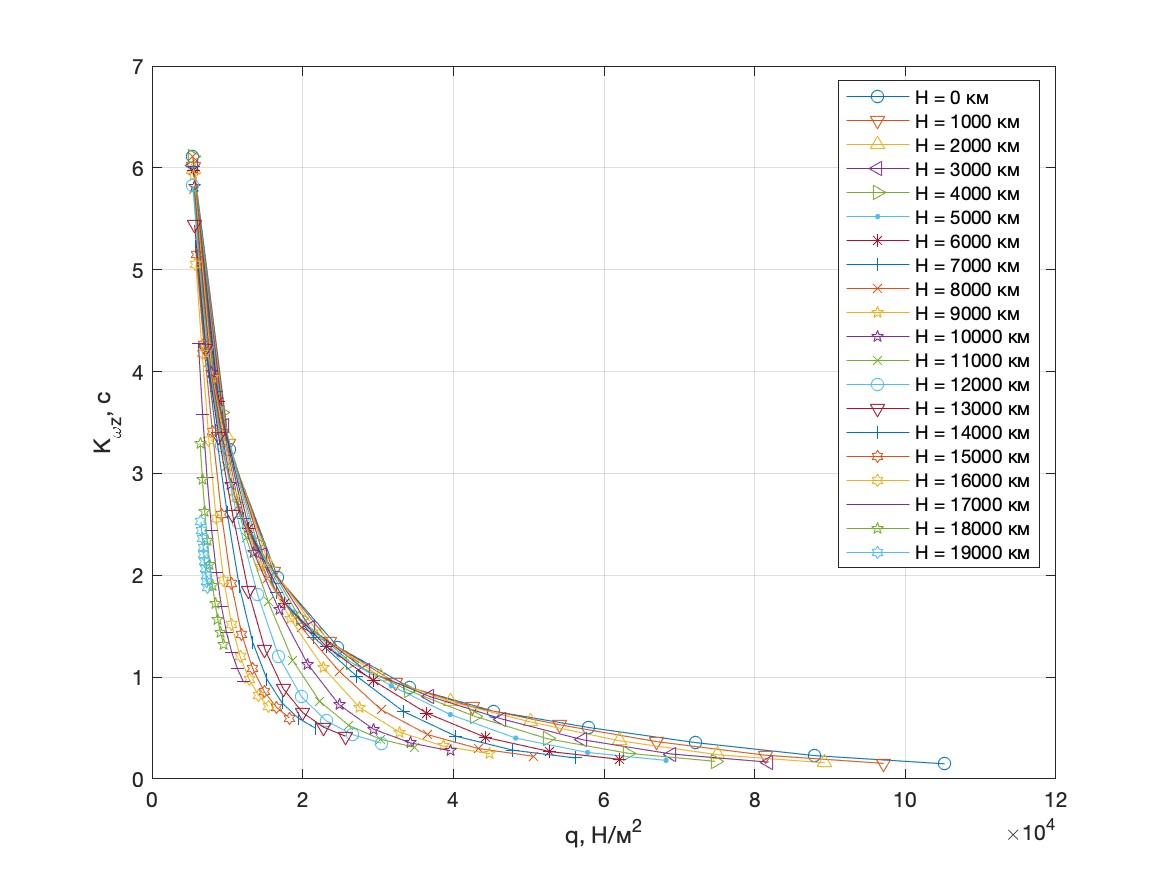
\includegraphics[width=\linewidth]{Оглавление/Part2/Sactions/Content/figures/K_wz.jpg}}
        \caption{$K_{\omega_z}(q), $с}
        \label{fig:K_wz}
    \end{figure}
    
    \begin{figure}[H]
        \center{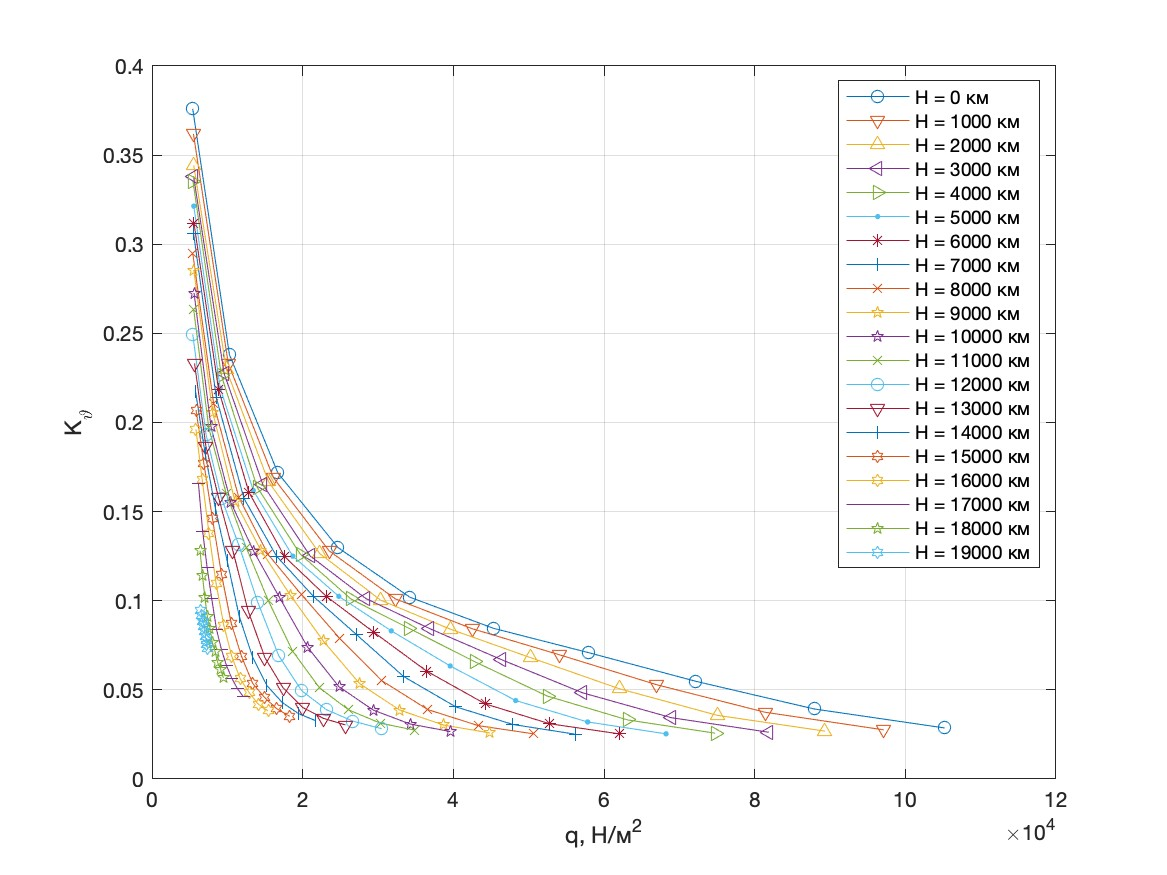
\includegraphics[width=\linewidth]{Оглавление/Part2/Sactions/Content/figures/K_v.jpg}}
        \caption{$K_{\vartheta}(q) $}
        \label{fig:K_wz}
    \end{figure}
    
    \subsubsection{Расчёты параметров для PI-контроллера}
    
    Передаточнвая функция разомкнутой системы стабилизации вертикальной скорости имеет вид:
    \begin{equation}
    \label{eq:ПФ разомкнутой системы стабилизации Vy}
        W^{V_y}_\text{раз}=R_H(p)\frac{K_H}{(\tau_1p+1)(\tau_2^2p^2+2\xi_2\tau_2p+1)}
    \end{equation}
    
    Из выражения (\ref{eq:ПФ разомкнутой системы стабилизации Vy}) следует, что система имеет собственную статическую ошибку. Устранение статической ошибки может быть достигнуто введением интеграла в закон управления. При этом передаточная функция регулятора принимает вид
    \begin{equation}
        \label{eq:PI-контроллер}
        R_{V_y}(p) = i_H + i_p\frac{1}{p}
    \end{equation}
    
    \subsubsubsection{Методика расчёта $i_H$ и $i_p$}
    
    Составим передаточную функцию учитывая соотношение (\ref{eq:PI-контроллер}) получим
    \begin{equation}
        \label{eq:ПФ с PI}
        W_\text{раз}^{V_{y}} = \frac{K_H (i_H+i_p\frac{1}{p})}{(\tau_1p+1)(\tau_2^2p^2+2\xi_2\tau_2p+1)}
    \end{equation}
    
    Преобразуем передаточную функцию (\ref{eq:ПФ с PI})
    
    \begin{equation}
        \label{eq:ПФ + PI преобразованная}
        W_\text{раз}^{V_y} = \frac{K_H i_p (\frac{i_H}{i_p}p + 1)}{p(\tau_1p+1)(\tau_2^2p^2+2\xi_2\tau_2p+1)}
    \end{equation}
    
    Из передаточной функции (\ref{eq:ПФ + PI преобразованная}) видно, что $\omega_{cp} \approx K_H i_p$. Делаем вывод, что 
    
    \begin{equation}
    \label{eq:i_p}
        i_p = 0,25 \frac{1}{\tau_1 K_H}
    \end{equation}
    
    Для уменьшения времени регулирования приравняем $\frac{i_H}{i_p} = \tau_1$
    
    \begin{equation}
        \label{eq:i_H}
        i_H = i_p \cdot \tau_1
    \end{equation}
    
    Подробнее об этом можно найти в учебнике \cite{UDLA}
    
    \begin{longtable}[H]{|c|c|c|c|c|c|c|c|c|c|c|}
    \caption[Результаты расчётов $i_p \cdot 10^{3}$,1/м в узловых точках]{Результаты расчётов $i_p \cdot 10^{3}$,1/м в узловых точках \label{tab:Результаты расчётов $i_p(H,M),$Н/м$^2$} \\
    \hline 
    $H,$ км &\multicolumn{10}{|c|}{$i_p \cdot 10^{3}$, 1/м } \\ \hline
    \endfirsthead
    
    \multicolumn{11}{c}%
    {{ \tablename\ \thetable{}: Результаты расчётов $i_p \cdot 10^{3}$,1/м в узловых точках}} \\
    \hline 
    $H,$ км &\multicolumn{10}{|c|}{$i_p \cdot 10^{3}$, 1/м } \\ \hline
    \endhead
    \endfoot
    
    \hline \hline
    \endlastfoot

    0 & 3,75 & 2,48 & 1,88 & 1,52 & 1,29 & 1,14 & 1,05 & 1,04 & 1,1 & 1,2  \\ \hline
    1 & 3,63 & 2,44 & 1,87 & 1,52 & 1,3 & 1,15 & 1,08 & 1,09 & 1,16 & 1,26  \\ \hline
    2 & 3,48 & 2,42 & 1,87 & 1,52 & 1,3 & 1,17 & 1,11 & 1,14 & 1,22 & 1,33  \\ \hline
    3 & 3,43 & 2,41 & 1,86 & 1,53 & 1,32 & 1,19 & 1,15 & 1,19 & 1,29 & 1,41  \\ \hline
    4 & 3,41 & 2,41 & 1,87 & 1,55 & 1,34 & 1,22 & 1,2 & 1,25 & 1,36 & 1,48  \\ \hline
    5 & 3,3 & 2,37 & 1,87 & 1,56 & 1,36 & 1,25 & 1,25 & 1,32 & 1,43 & 1,55  \\ \hline
    6 & 3,22 & 2,37 & 1,88 & 1,57 & 1,38 & 1,3 & 1,31 & 1,4 & 1,51 & 1,63  \\ \hline
    7 & 3,18 & 2,36 & 1,87 & 1,59 & 1,41 & 1,35 & 1,38 & 1,47 & 1,59 & 1,7  \\ \hline
    8 & 3,1 & 2,35 & 1,9 & 1,62 & 1,46 & 1,4 & 1,45 & 1,55 & 1,66 & 1,77  \\ \hline
    9 & 3,04 & 2,33 & 1,9 & 1,65 & 1,5 & 1,48 & 1,54 & 1,64 & 1,74 & 1,82  \\ \hline
    10 & 2,95 & 2,29 & 1,91 & 1,68 & 1,56 & 1,55 & 1,62 & 1,72 & 1,81 & 1,88  \\ \hline
    11 & 2,91 & 2,32 & 1,98 & 1,74 & 1,63 & 1,64 & 1,72 & 1,81 & 1,88 & 1,93  \\ \hline
    12 & 2,82 & 2,31 & 1,98 & 1,82 & 1,73 & 1,73 & 1,8 & 1,89 & 1,95 & 1,98  \\ \hline
    13 & 2,71 & 2,27 & 2,03 & 1,89 & 1,81 & 1,83 & 1,89 & 1,94 & 2 & 2,03  \\ \hline
    14 & 2,59 & 2,26 & 2,05 & 1,96 & 1,91 & 1,94 & 1,97 & 2,03 & 2,06 & 2,08  \\ \hline
    15 & 2,52 & 2,29 & 2,13 & 2,05 & 2,02 & 2,05 & 2,06 & 2,11 & 2,12 & 2,13  \\ \hline
    16 & 2,49 & 2,34 & 2,24 & 2,19 & 2,17 & 2,17 & 2,16 & 2,19 & 2,18 & 2,19  \\ \hline
    17 & 2,47 & 2,37 & 2,34 & 2,33 & 2,28 & 2,29 & 2,29 & 2,29 & 2,28 & 2,28  \\ \hline
    18 & 2,54 & 2,5 & 2,45 & 2,42 & 2,44 & 2,41 & 2,42 & 2,39 & 2,4 & 2,38  \\ \hline
    19  & 2,59 & 2,58 & 2,56 & 2,61 & 2,59 & 2,58 & 2,57 & 2,55 & 2,54 & 2,53 \\ \hline
    \end{longtable}

        
  \begin{longtable}[H]{|c|c|c|c|c|c|c|c|c|c|c|}
    \caption[Результаты расчётов $i_H \cdot 10^{3}$,1/м в узловых точках]{Результаты расчётов $i_H \cdot 10^{3}$,1/м в узловых точках \label{tab:Результаты расчётов $i_H(H,M),$Н/м$^2$} \\
    \hline 
    $H,$ км &\multicolumn{10}{|c|}{$i_H \cdot 10^{3}$, 1/м } \\ \hline
    \endfirsthead
    
    \multicolumn{11}{c}%
    {{ \tablename\ \thetable{}: Результаты расчётов $i_H \cdot 10^{3}$,1/м в узловых точках}} \\
    \hline 
    $H,$ км &\multicolumn{10}{|c|}{$i_H \cdot 10^{3}$, 1/м } \\ \hline
    \endhead
    \endfoot
    
    \hline \hline
    \endlastfoot

    0 & 0,99 & 0,89 & 0,86 & 0,84 & 0,84 & 0,86 & 0,9 & 1 & 1,19 & 1,49  \\ \hline
    1 & 0,92 & 0,83 & 0,8 & 0,78 & 0,79 & 0,8 & 0,85 & 0,96 & 1,16 & 1,46  \\ \hline
    2 & 0,84 & 0,77 & 0,74 & 0,73 & 0,73 & 0,75 & 0,8 & 0,92 & 1,13 & 1,43  \\ \hline
    3 & 0,78 & 0,72 & 0,69 & 0,67 & 0,68 & 0,7 & 0,76 & 0,89 & 1,1 & 1,4  \\ \hline
    4 & 0,73 & 0,67 & 0,64 & 0,63 & 0,63 & 0,65 & 0,72 & 0,86 & 1,06 & 1,36  \\ \hline
    5 & 0,68 & 0,61 & 0,59 & 0,58 & 0,59 & 0,61 & 0,69 & 0,83 & 1,04 & 1,32  \\ \hline
    6 & 0,62 & 0,58 & 0,55 & 0,54 & 0,55 & 0,58 & 0,66 & 0,8 & 1,01 & 1,28  \\ \hline
    7 & 0,58 & 0,53 & 0,51 & 0,5 & 0,51 & 0,55 & 0,63 & 0,77 & 0,97 & 1,22  \\ \hline
    8 & 0,53 & 0,49 & 0,47 & 0,46 & 0,48 & 0,52 & 0,61 & 0,74 & 0,93 & 1,16  \\ \hline
    9 & 0,49 & 0,46 & 0,44 & 0,43 & 0,45 & 0,49 & 0,58 & 0,71 & 0,88 & 1,07  \\ \hline
    10 & 0,45 & 0,42 & 0,4 & 0,4 & 0,42 & 0,47 & 0,55 & 0,68 & 0,83 & 0,99  \\ \hline
    11 & 0,42 & 0,39 & 0,38 & 0,38 & 0,39 & 0,44 & 0,53 & 0,64 & 0,77 & 0,91  \\ \hline
    12 & 0,37 & 0,35 & 0,34 & 0,35 & 0,37 & 0,41 & 0,49 & 0,59 & 0,71 & 0,81  \\ \hline
    13 & 0,34 & 0,32 & 0,31 & 0,32 & 0,34 & 0,38 & 0,45 & 0,52 & 0,62 & 0,7  \\ \hline
    14 & 0,3 & 0,29 & 0,29 & 0,3 & 0,32 & 0,36 & 0,41 & 0,47 & 0,54 & 0,61  \\ \hline
    15 & 0,27 & 0,27 & 0,27 & 0,28 & 0,3 & 0,34 & 0,37 & 0,43 & 0,48 & 0,53  \\ \hline
    16 & 0,25 & 0,25 & 0,26 & 0,27 & 0,29 & 0,31 & 0,34 & 0,38 & 0,42 & 0,46  \\ \hline
    17 & 0,24 & 0,24 & 0,25 & 0,26 & 0,27 & 0,29 & 0,31 & 0,33 & 0,35 & 0,37  \\ \hline
    18 & 0,23 & 0,24 & 0,24 & 0,25 & 0,26 & 0,26 & 0,27 & 0,28 & 0,3 & 0,3  \\ \hline
    19  & 0,23 & 0,23 & 0,23 & 0,24 & 0,24 & 0,24 & 0,25 & 0,25 & 0,25 & 0,25 \\ \hline
    \end{longtable}


\begin{figure}[H]
        \center{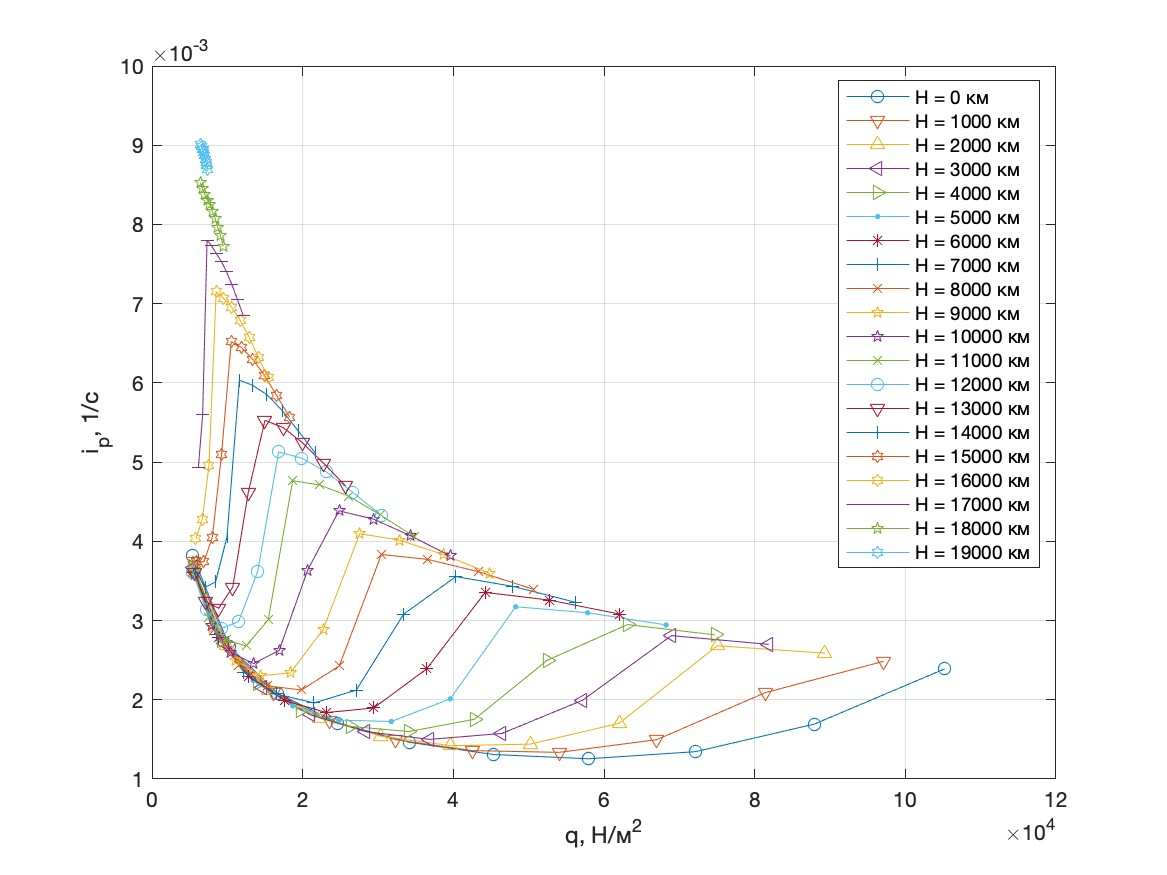
\includegraphics[width=\linewidth]{Оглавление/Part2/Sactions/Content/figures/i_p.jpg}}
        \caption{$i_p(q), $1/м}
        \label{fig:i_p}
    \end{figure} 

\begin{figure}[H]
        \center{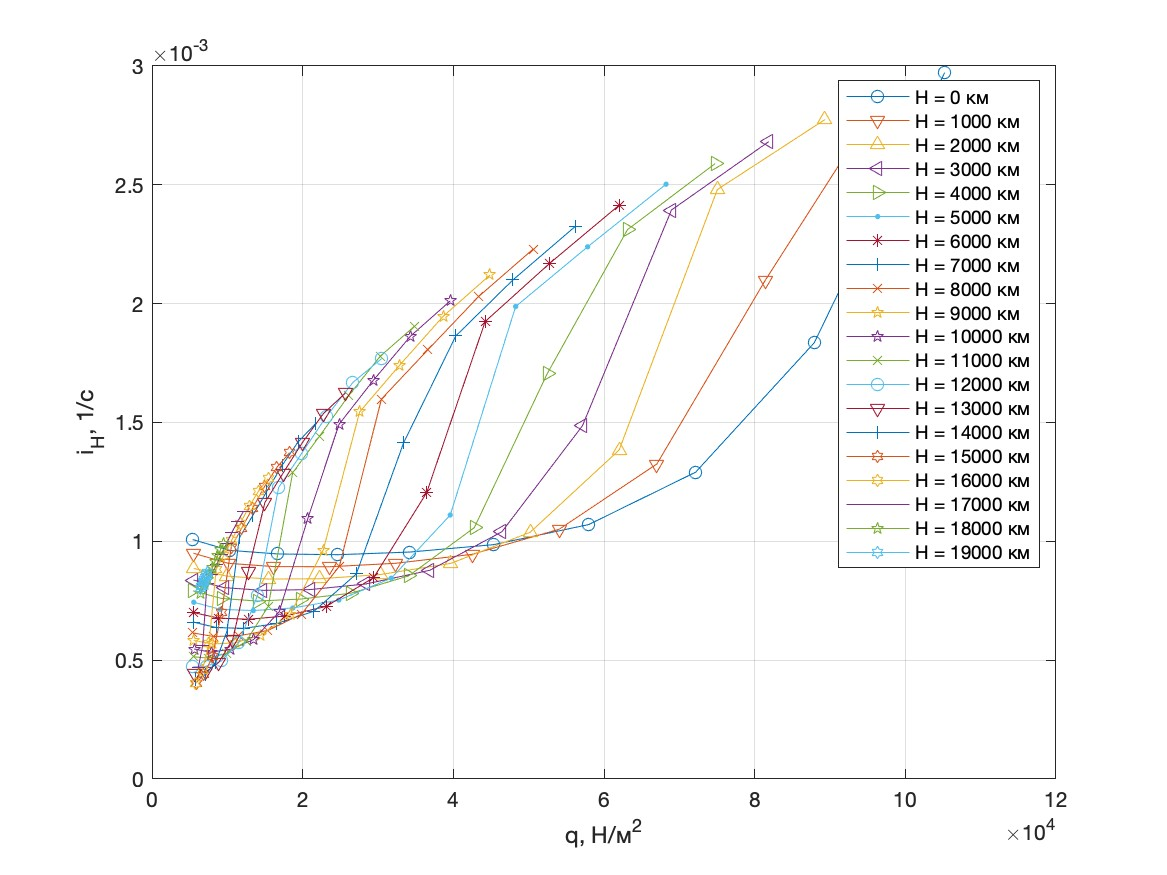
\includegraphics[width=\linewidth]{Оглавление/Part2/Sactions/Content/figures/i_H.jpg}}
        \caption{$i_H(q), $1/м}
        \label{fig:i_H}
    \end{figure} 
    

Для выполнения частотного анализа, который производится в следующем подразделе, необходимо по вышеприведенным графикам и таблицам определить коэффициенты обратных связей при минимальной скоростном напоре, максимальном скоростном напоре и скоростном напоре крейсерского полета. Значения найденных коэффициентов оформлены в виде таблиц \ref{tab:q_min} - \ref{tab:q_kr}


\begin{table}[H]
    \centering
    \caption{Коэффициенты обратных связей, соответствующие $q_{min}$}
    \begin{tabular}{|c|c|c|c|c|c|c|c|}
    \hline
        $H,$ км & $M$ & $q, H / \text{м}^2$ & $K_{\omega_z}, c$ & $K_\vartheta$ & $K_H,$м/c &$i_H$&$i_p$\\ \hline
        0& 0,2760& 5403  &5,31 & 30,472&156,1 &7,8$\cdot 10^{-2}$&1,14 $\cdot 10^{-2}$\\ \hline
    \end{tabular}
    \label{tab:q_min}
\end{table}

\begin{table}[H]
    \centering
    \caption{Коэффициенты обратных связей, соответствующие $q_{max}$}
    \begin{tabular}{|c|c|c|c|c|c|c|c|}
    \hline
        $H,$ км & $M$ & $q, H / \text{м}^2$ & $K_{\omega_z}, c$ & $K_\vartheta$ & $K_H,$м/c &$i_H$&$i_p$ \\ \hline
        0& 1,0976 &105220& 0,3545 & 2,035&340,4&3,6 $\cdot 10^{-3}$&3,4 $\cdot 10^{-3}$\\ \hline
    \end{tabular}
    \label{tab:q_max}
\end{table}


\begin{table}[H]
    \centering
    \caption{Коэффициенты обратных связей, соответствующие $q_\text{кр}$}
    \begin{tabular}{|c|c|c|c|c|c|c|c|}
    \hline
        $H,$ км & $M$ & $q, H / \text{м}^2$ & $K_{\omega_z}, c$ & $K_\vartheta$ & $K_H,$м/c &$i_H$&$i_p$ \\ \hline
        17&0,928&5438 &3,157 & 1,1 &222,0199 &2,8 $\cdot 10^{-3}$&4,4 $\cdot 10^{-4}$\\ \hline
    \end{tabular}
    \label{tab:q_kr}
\end{table}

\begin{center}
    Выводы:
\end{center}

Полученные значения коэффициентов обратных связей были успешно найдены и применены на модели рассматриваемой системы стабилизации вертикальной скорости в системе «Simulink». Моделирование показало, что коэффициенты найдены верно, так как заданная вертикальная скорость равена вертикальной скорости на выходе из системы. Более подробно будут показаны результаты моделирования и сама модель в разделе «Нелинейное моделирование» (раздел 3).

\subsubsection{Частотный анализ}

Целью частотного анализа является построение логарифмических амплитудных и фазовых частотных характеристик (ЛАФЧХ) разомкнутых и замкнутых контуров управления до синтеза и после синтеза и проведение их сравнительного анализа.
% ________________________________________________________________________________________________
\subsubsubsection{Частотный анализ $q_{min}$}

\begin{center}
    Контур демпфирования угловой скорости тангажа:
\end{center}

\begin{figure}[H]
    \center{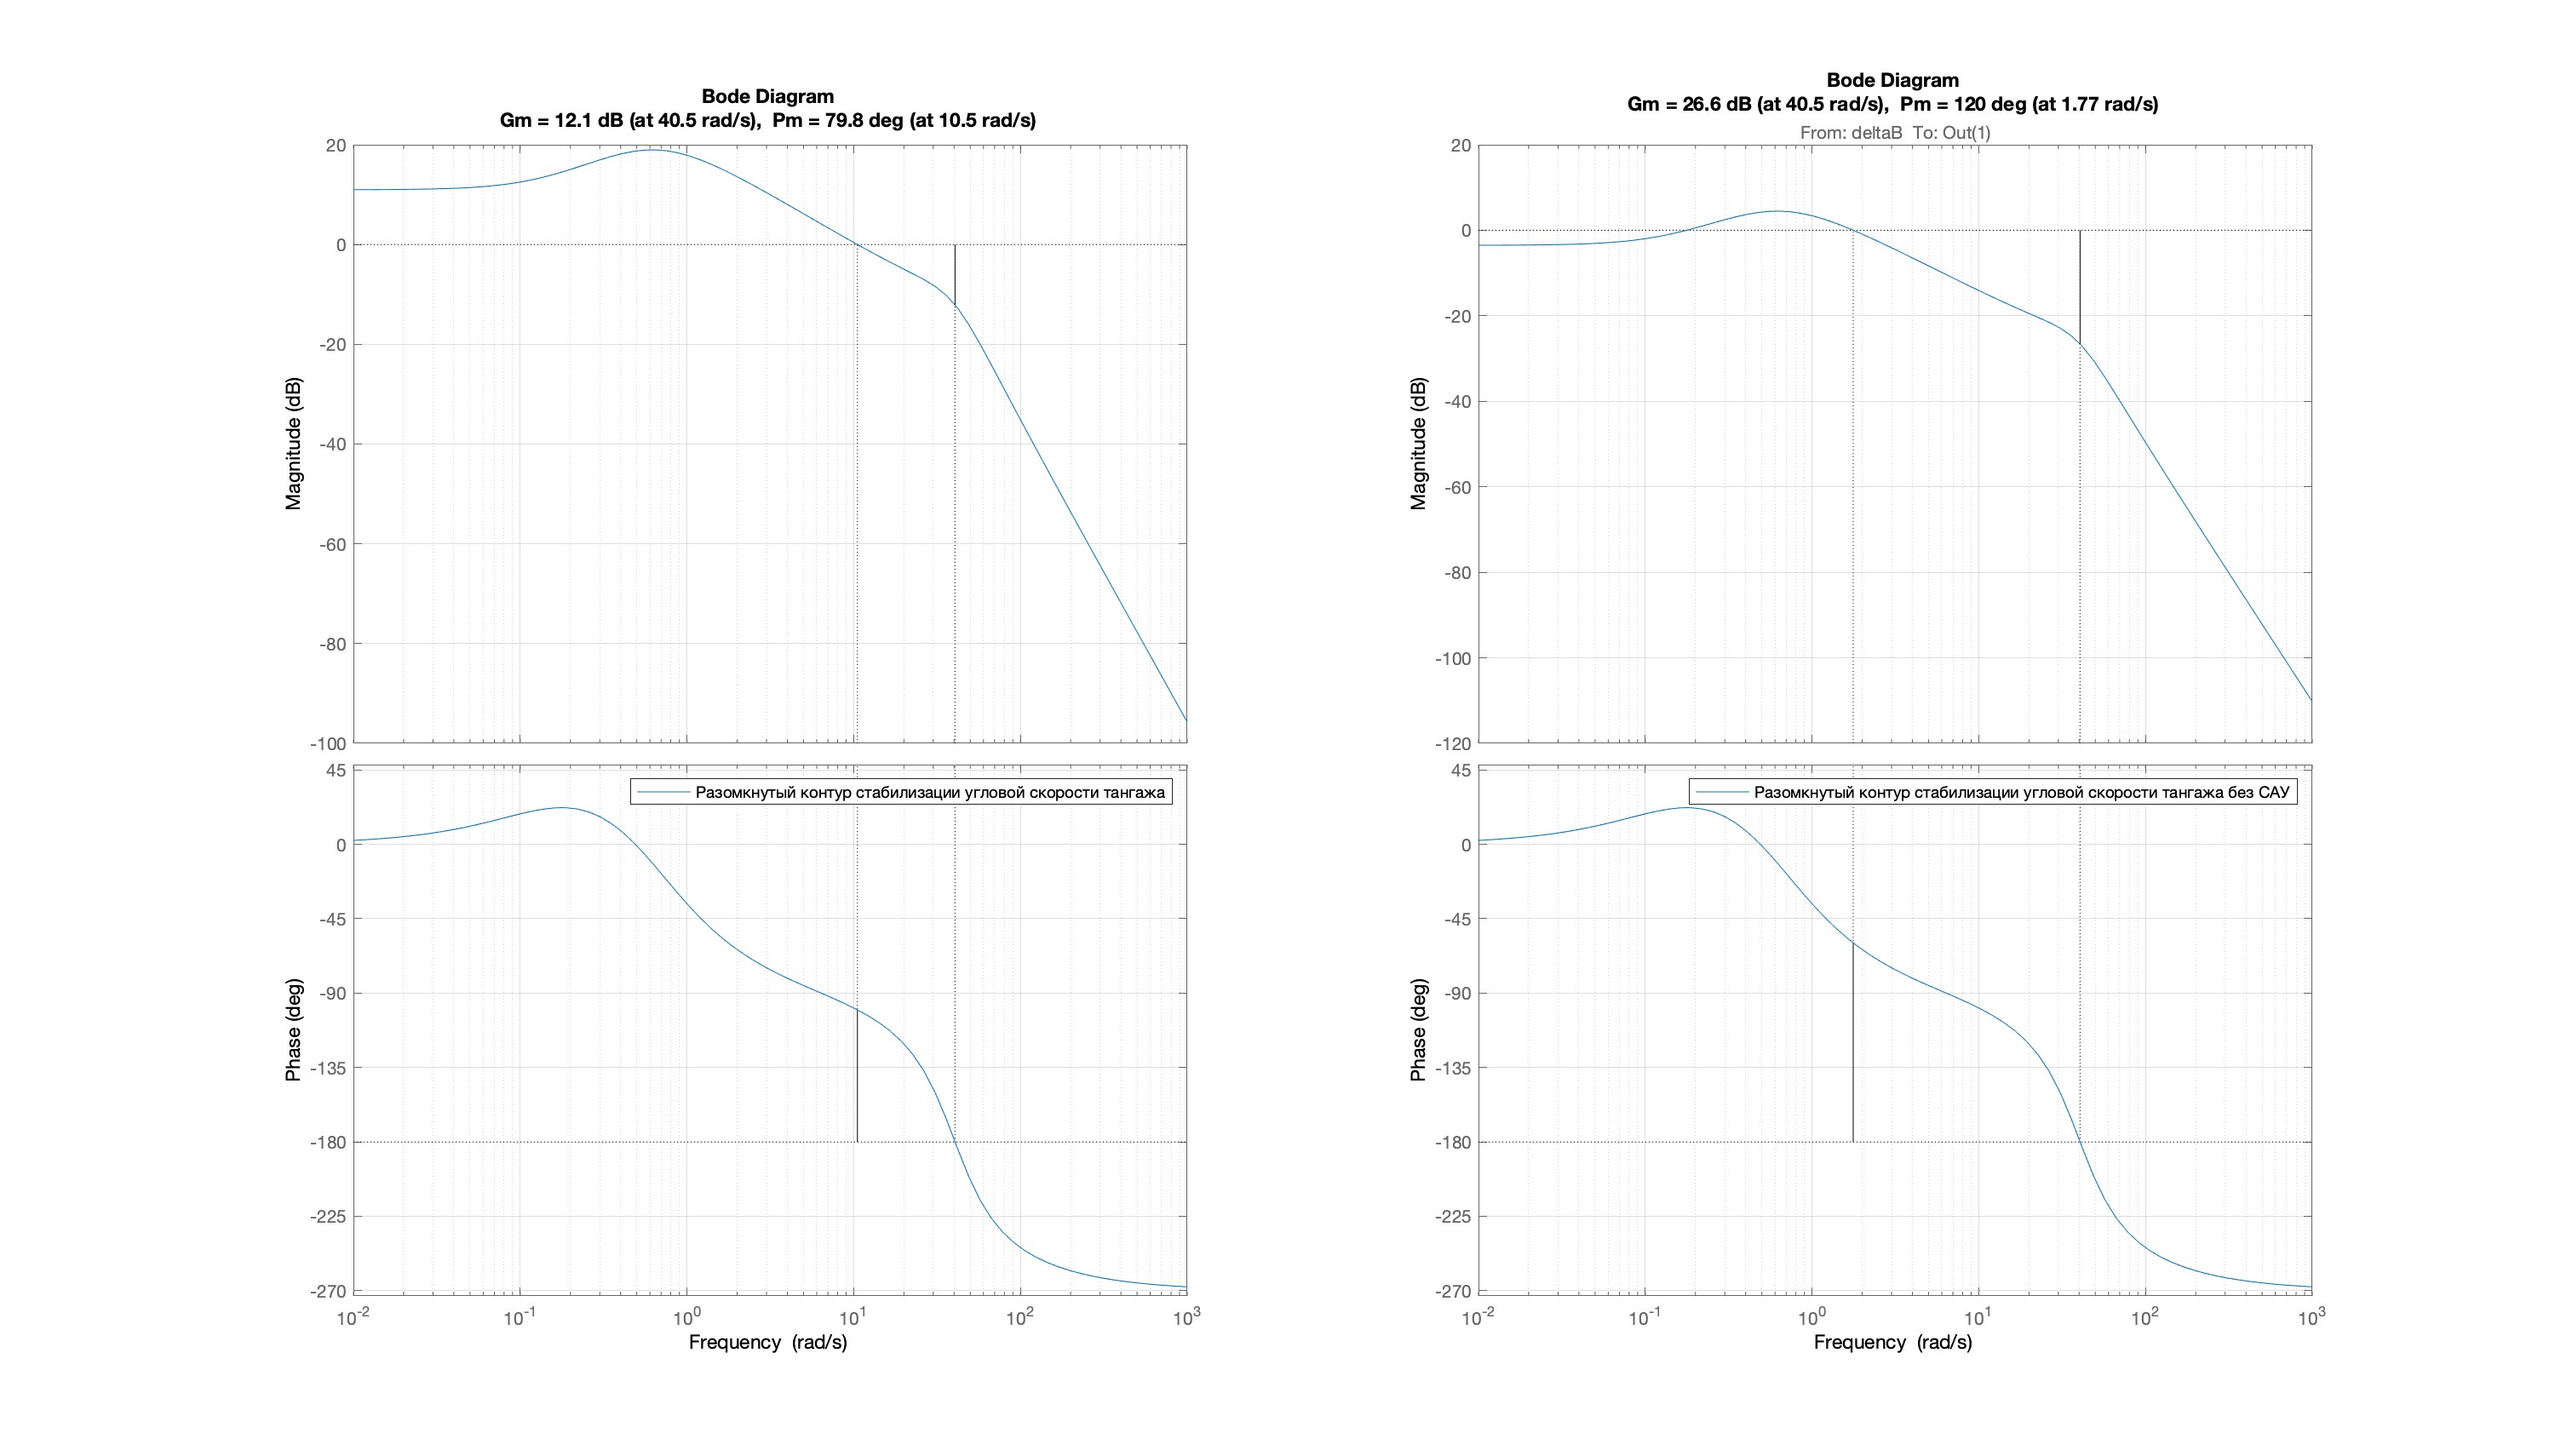
\includegraphics[width=\linewidth]{Оглавление/Part2/Sactions/Content/frequencies/Угловая скорость тангажа раз qMIN.jpg}}
    \caption{ЛАФЧХ разомкнутого контура демпфирования угловой скорости тангажа}
    \label{fig:Угловая скорость тангажа раз qMIN}
\end{figure}

Из рисунка \ref{fig:Угловая скорость тангажа раз qMIN} видно, что до синтеза данного контура запасы устойчивости по амплитуде и по фазе не удовлетворяют заданным требованиям, то есть запас по амплитуде меньше 10 дб и запас по фазе меньше 45 град, а после синтеза $\Delta A = 12,3$дБ $\Delta \varphi = 80^0$, следовательно, синтез проведен успешно, коэффициенты рассчитаны верно. Замкнутая система будет устойчива. Частота среза после синтеза не превысила граничного значения, она находится на участке с наклоном -20дб/дек, чего и требовалось достичь в результате синтеза.  

\begin{center}
    Контур стабилизации тангажа:
\end{center}

\begin{figure}[H]
    \center{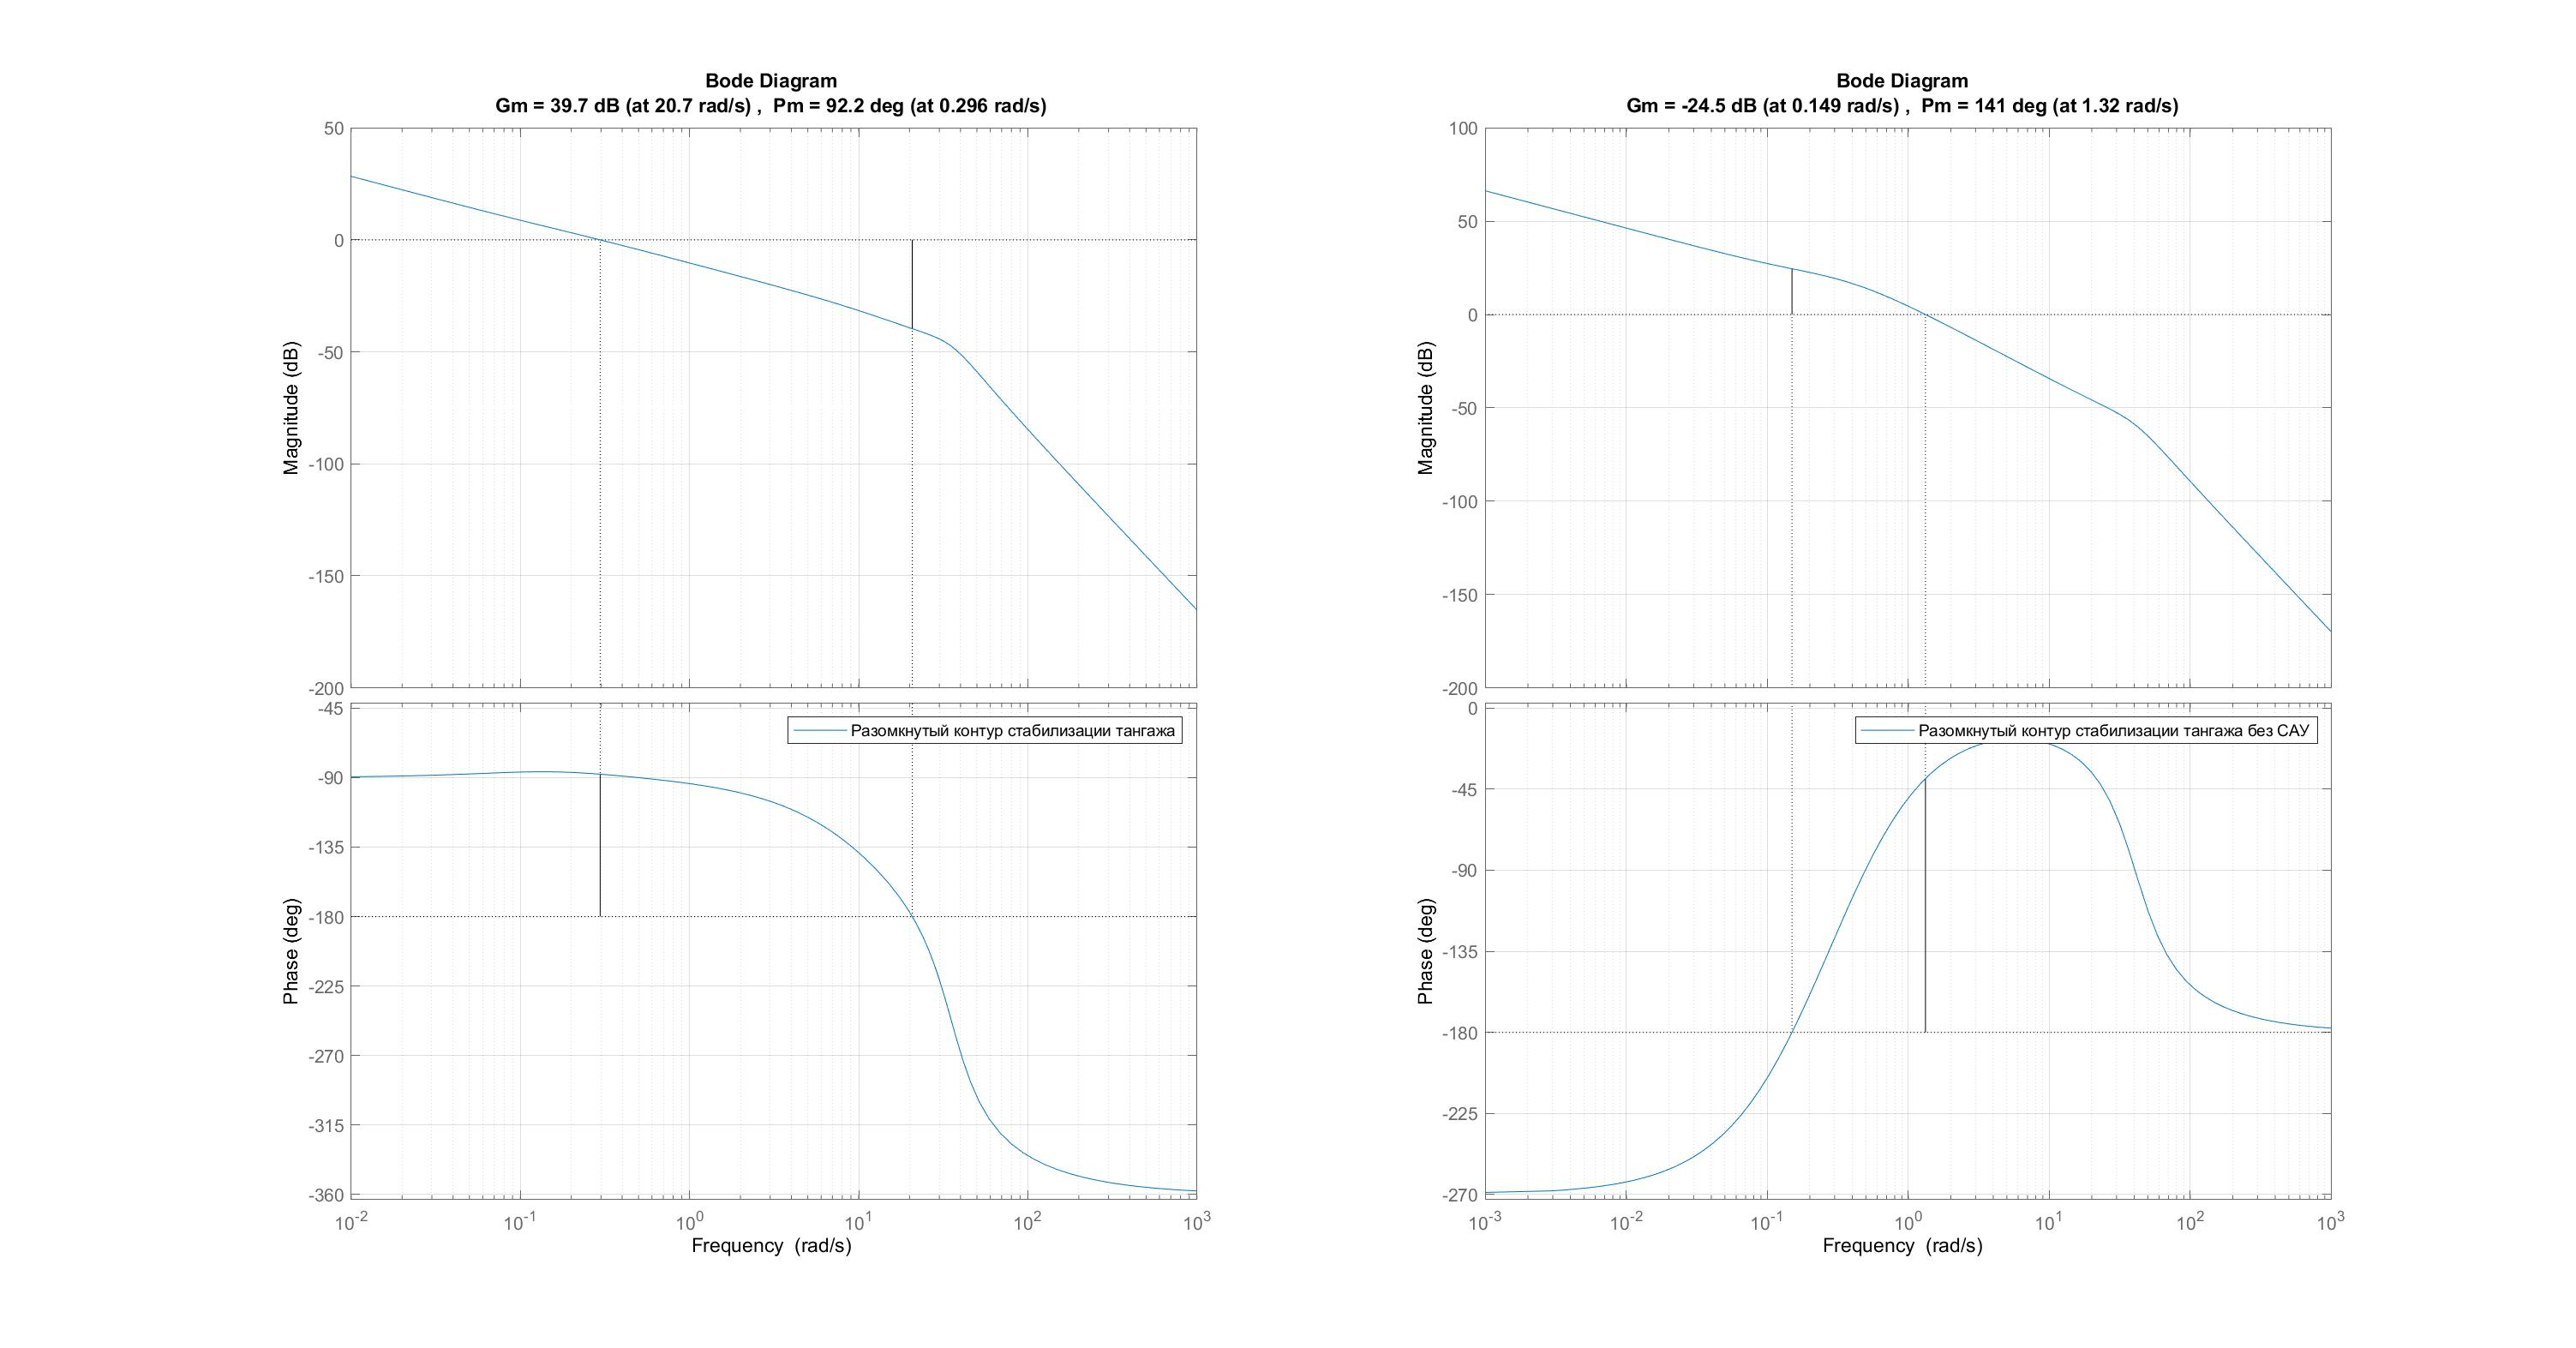
\includegraphics[width=\linewidth]{Оглавление/Part2/Sactions/Content/frequencies/Тангаж раз qMIN.jpg}}
    \caption{ЛАФЧХ разомкнутого контура стабилизации тангажа}
    \label{fig:Тангаж раз qMIN}
\end{figure}

Из рисунка \ref{fig:Тангаж раз qMIN} видно, что до синтеза данного контура запасы устойчивости по амплитуде и по фазе не удовлетворяют заданным требованиям, то есть запас по амплитуде меньше 10 дб и запас по фазе меньше 45 град, а после синтеза $\Delta A = 39,7 $дБ $\Delta \varphi = 92^0$, следовательно, синтез проведен успешно, коэффициенты рассчитаны верно. Замкнутая система будет устойчива.  

\begin{center}
    Контур вертикальной скорости:
\end{center}

\begin{figure}[H]
    \center{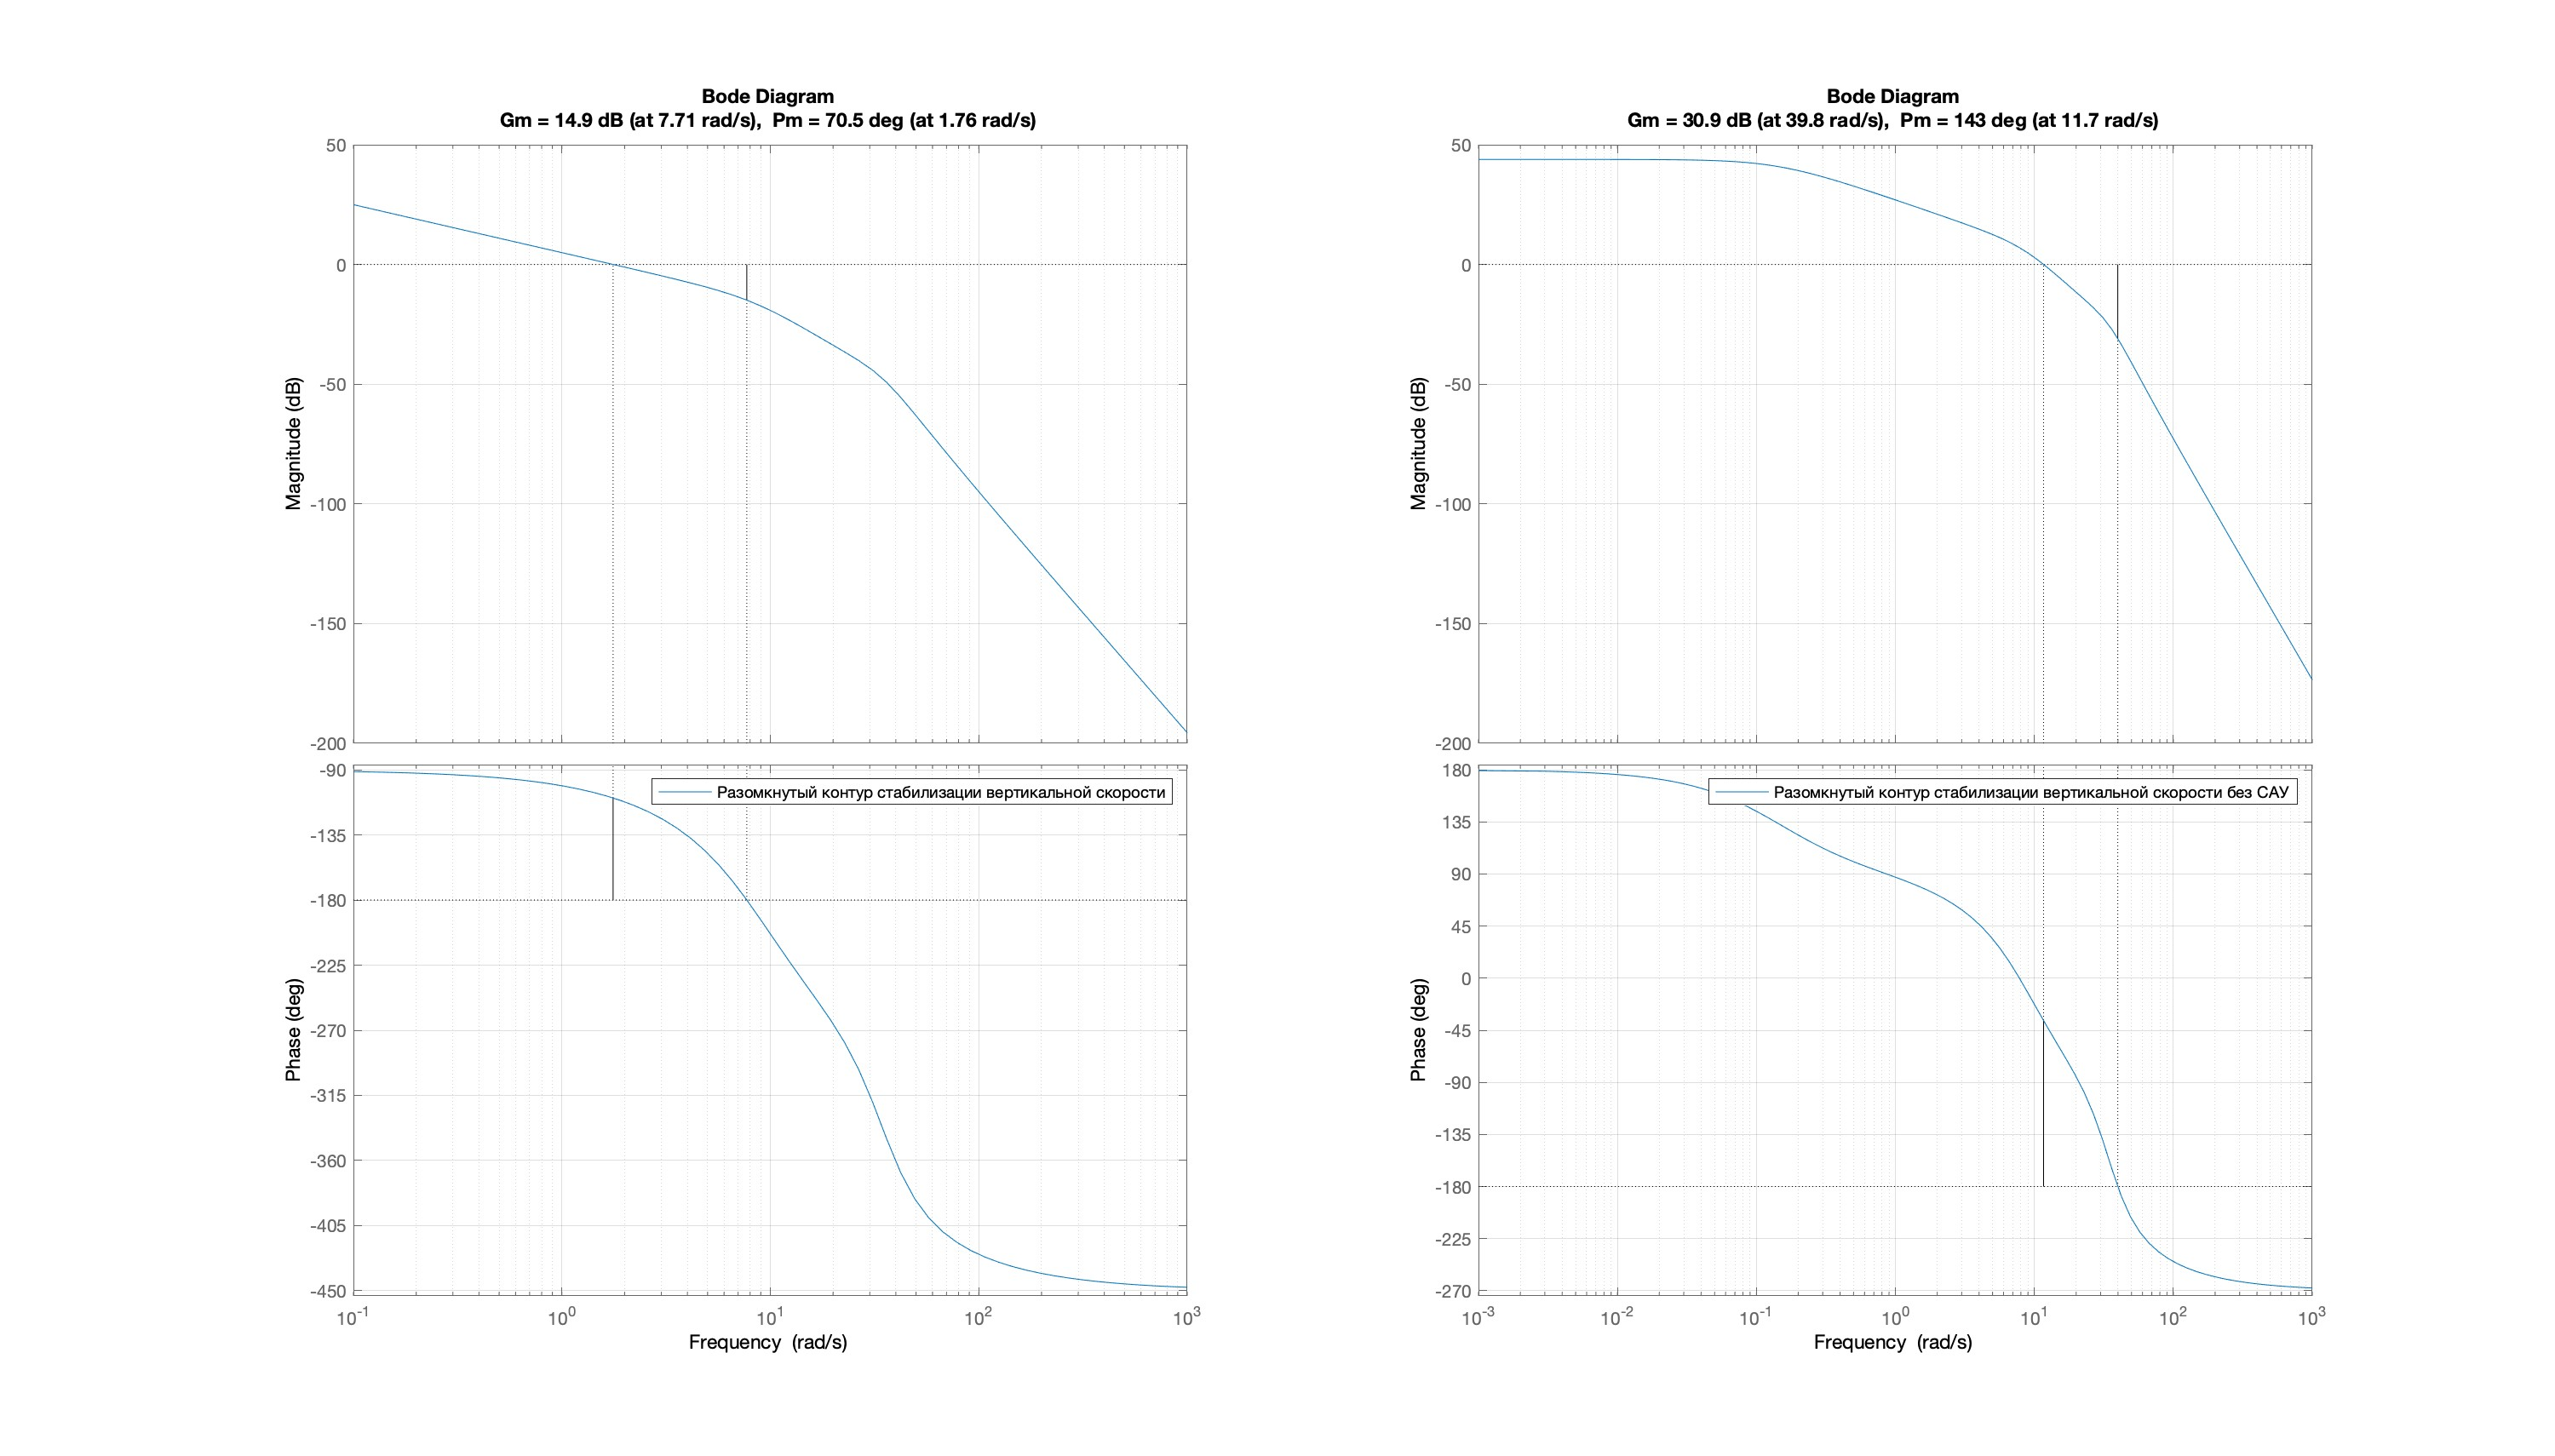
\includegraphics[width=\linewidth]{Оглавление/Part2/Sactions/Content/frequencies/Вертикальная скорость раз qMIN.jpg}}
    \caption{ЛАФЧХ разомкнутого контура стабилизации вертикальной скорости}
    \label{fig:Вертикальная скорость раз qMIN}
\end{figure}

Из рисунка \ref{fig:Вертикальная скорость раз qMIN} видно, что после синтеза $\Delta A = 42,2 $дБ $\Delta \varphi = 73^0$, следовательно, синтез проведен успешно, коэффициенты рассчитаны верно. Замкнутая система будет устойчива. 

\begin{figure}[H]
    \center{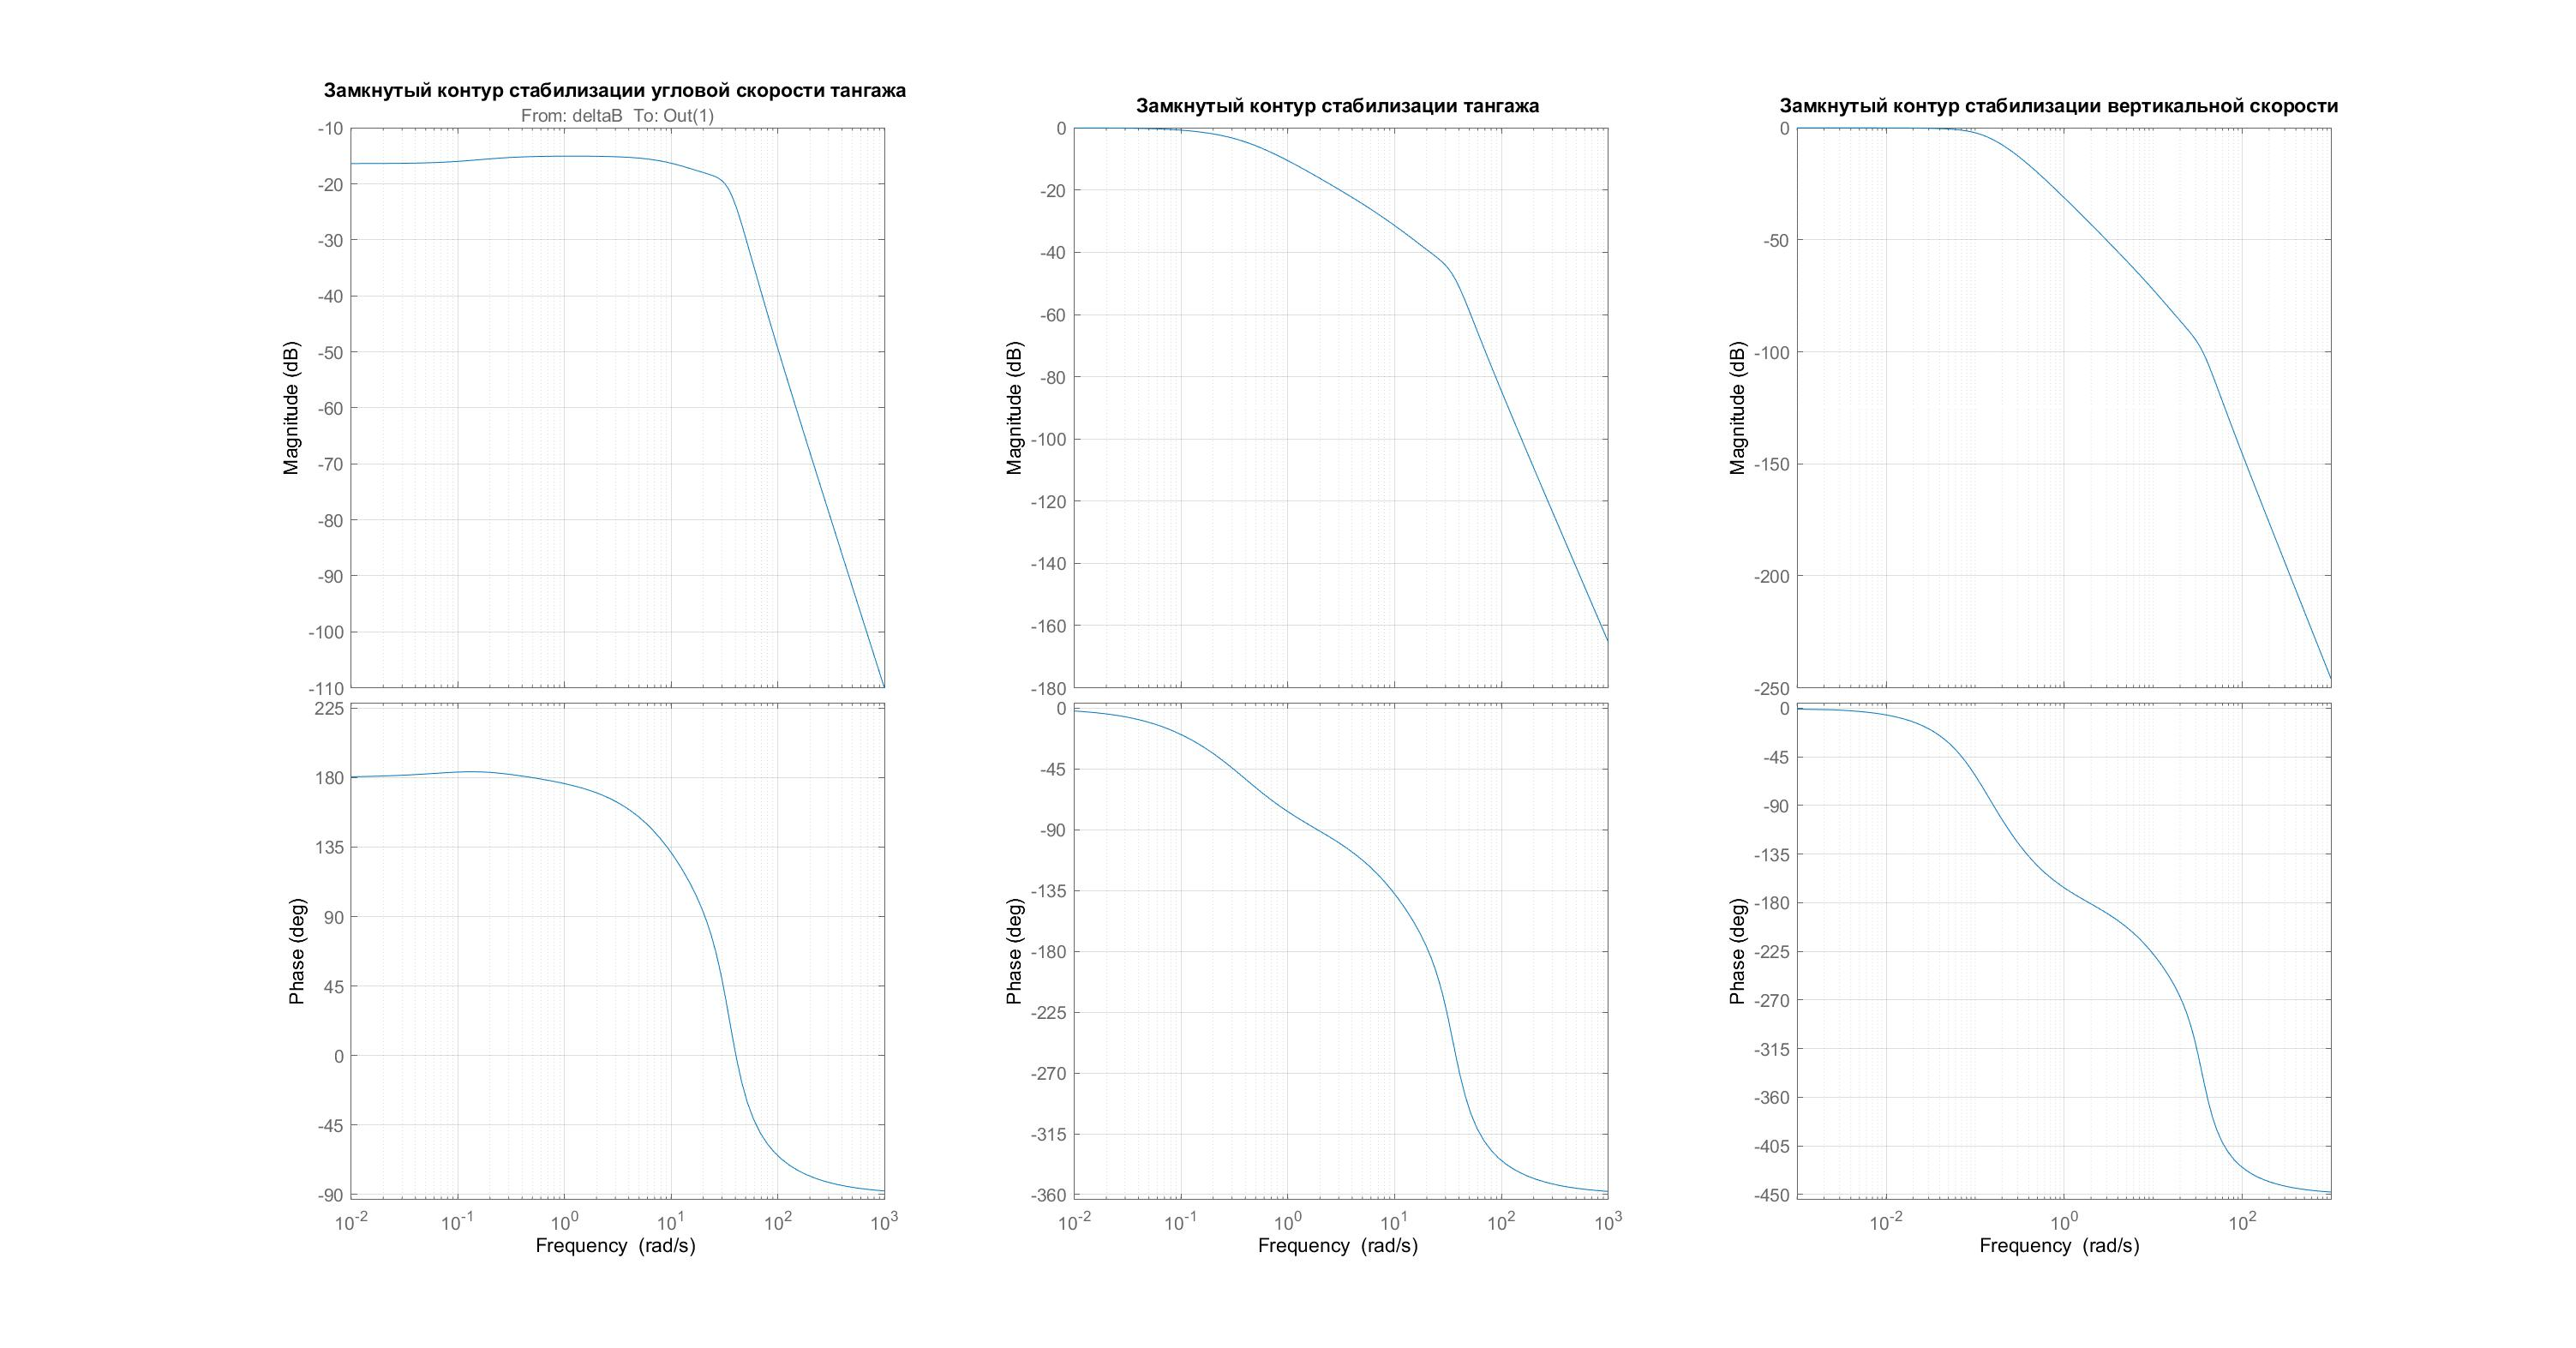
\includegraphics[width=\linewidth]{Оглавление/Part2/Sactions/Content/frequencies/ZAM qMIN.jpg}}
    \caption{ЛАФЧХ замкнутого контура }
    \label{fig:Вертикальная скорость зам qMIN}
\end{figure}
% __________________________________________________________________________________________
\subsubsubsection{Частотный анализ $q_{max}$}

\begin{center}
    Контур демпфирования угловой скорости тангажа:
\end{center}

\begin{figure}[H]
    \center{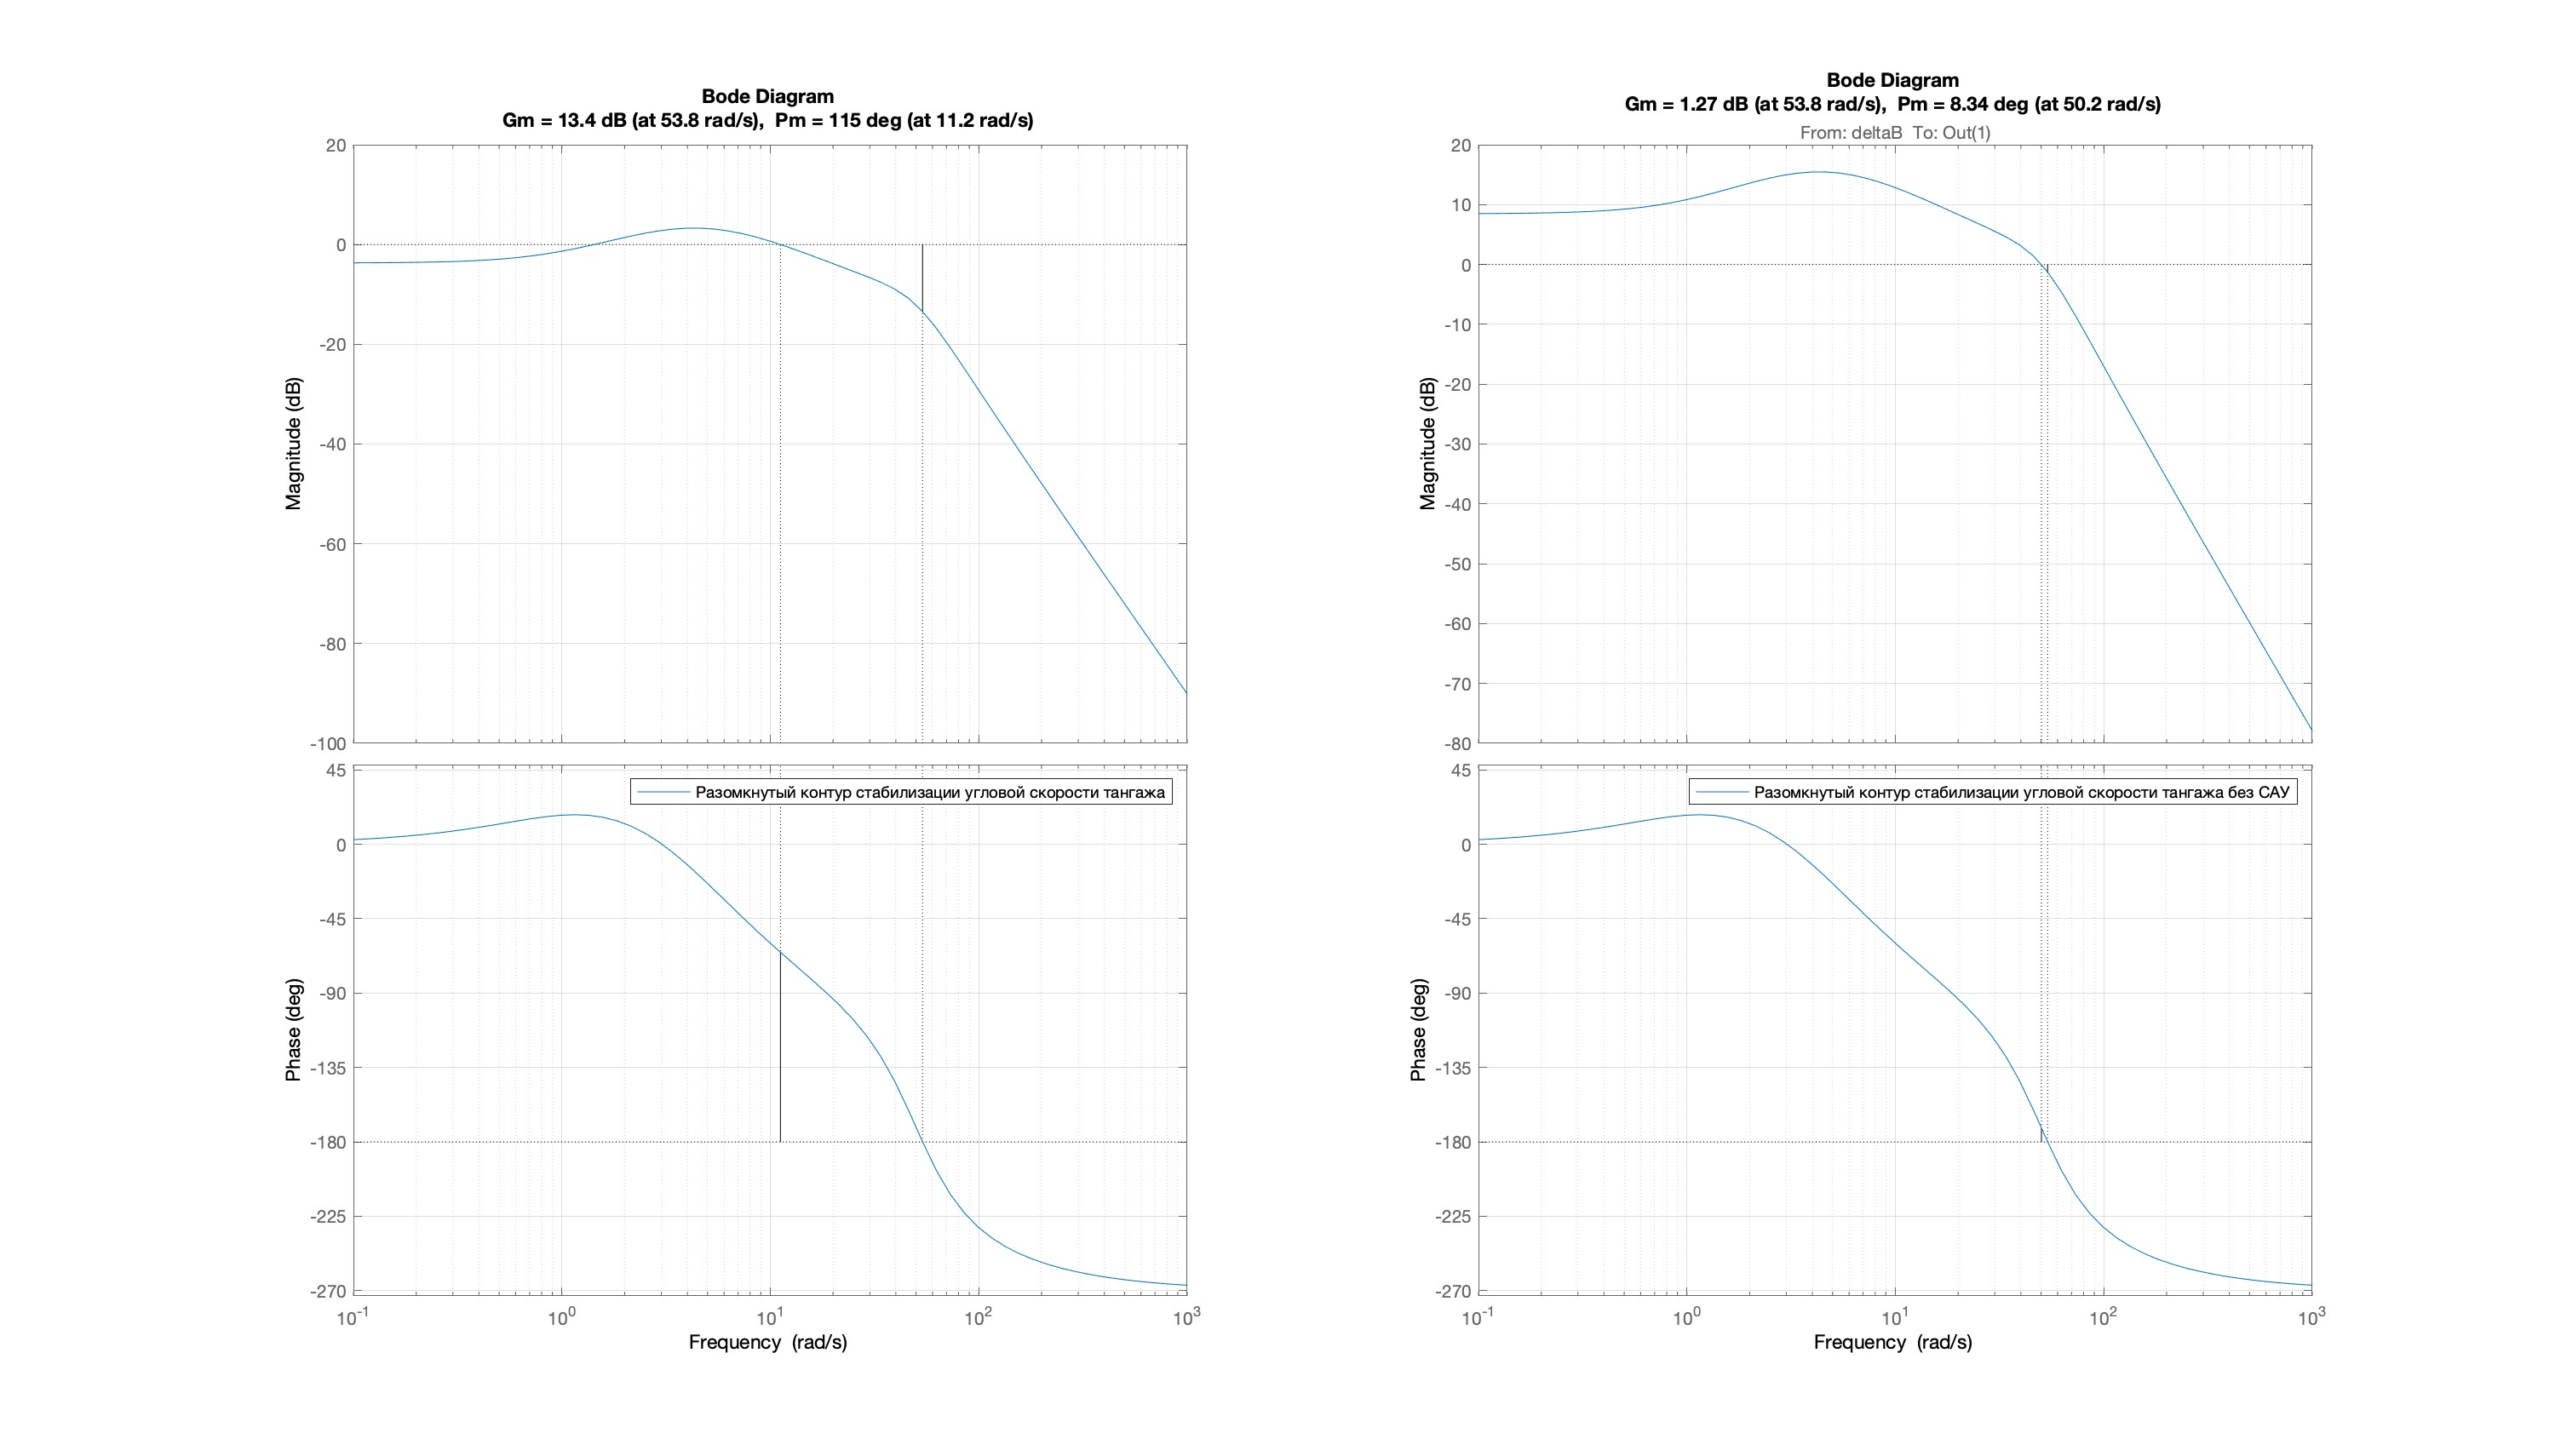
\includegraphics[width=\linewidth]{Оглавление/Part2/Sactions/Content/frequencies/Угловая скорость тангажа раз qMAX.jpg}}
    \caption{ЛАФЧХ разомкнутого контура демпфирования угловой скорости тангажа}
    \label{fig:Угловая скорость тангажа раз qMAX}
\end{figure}

Из рисунка \ref{fig:Угловая скорость тангажа раз qMAX} видно, что до синтеза данного контура запасы устойчивости по амплитуде и по фазе не удовлетворяют заданным требованиям, то есть запас по амплитуде меньше 10 дб и запас по фазе меньше 45 град, а после синтеза $\Delta A = 13,7 $дБ $\Delta \varphi = 124^0$, следовательно, синтез проведен успешно, коэффициенты рассчитаны верно. Замкнутая система будет устойчива. Частота среза после синтеза не превысила граничного значения, она находится на участке с наклоном -20дб/дек, чего и требовалось достичь в результате синтеза.  

\begin{center}
    Контур стабилизации тангажа:
\end{center}

\begin{figure}[H]
    \center{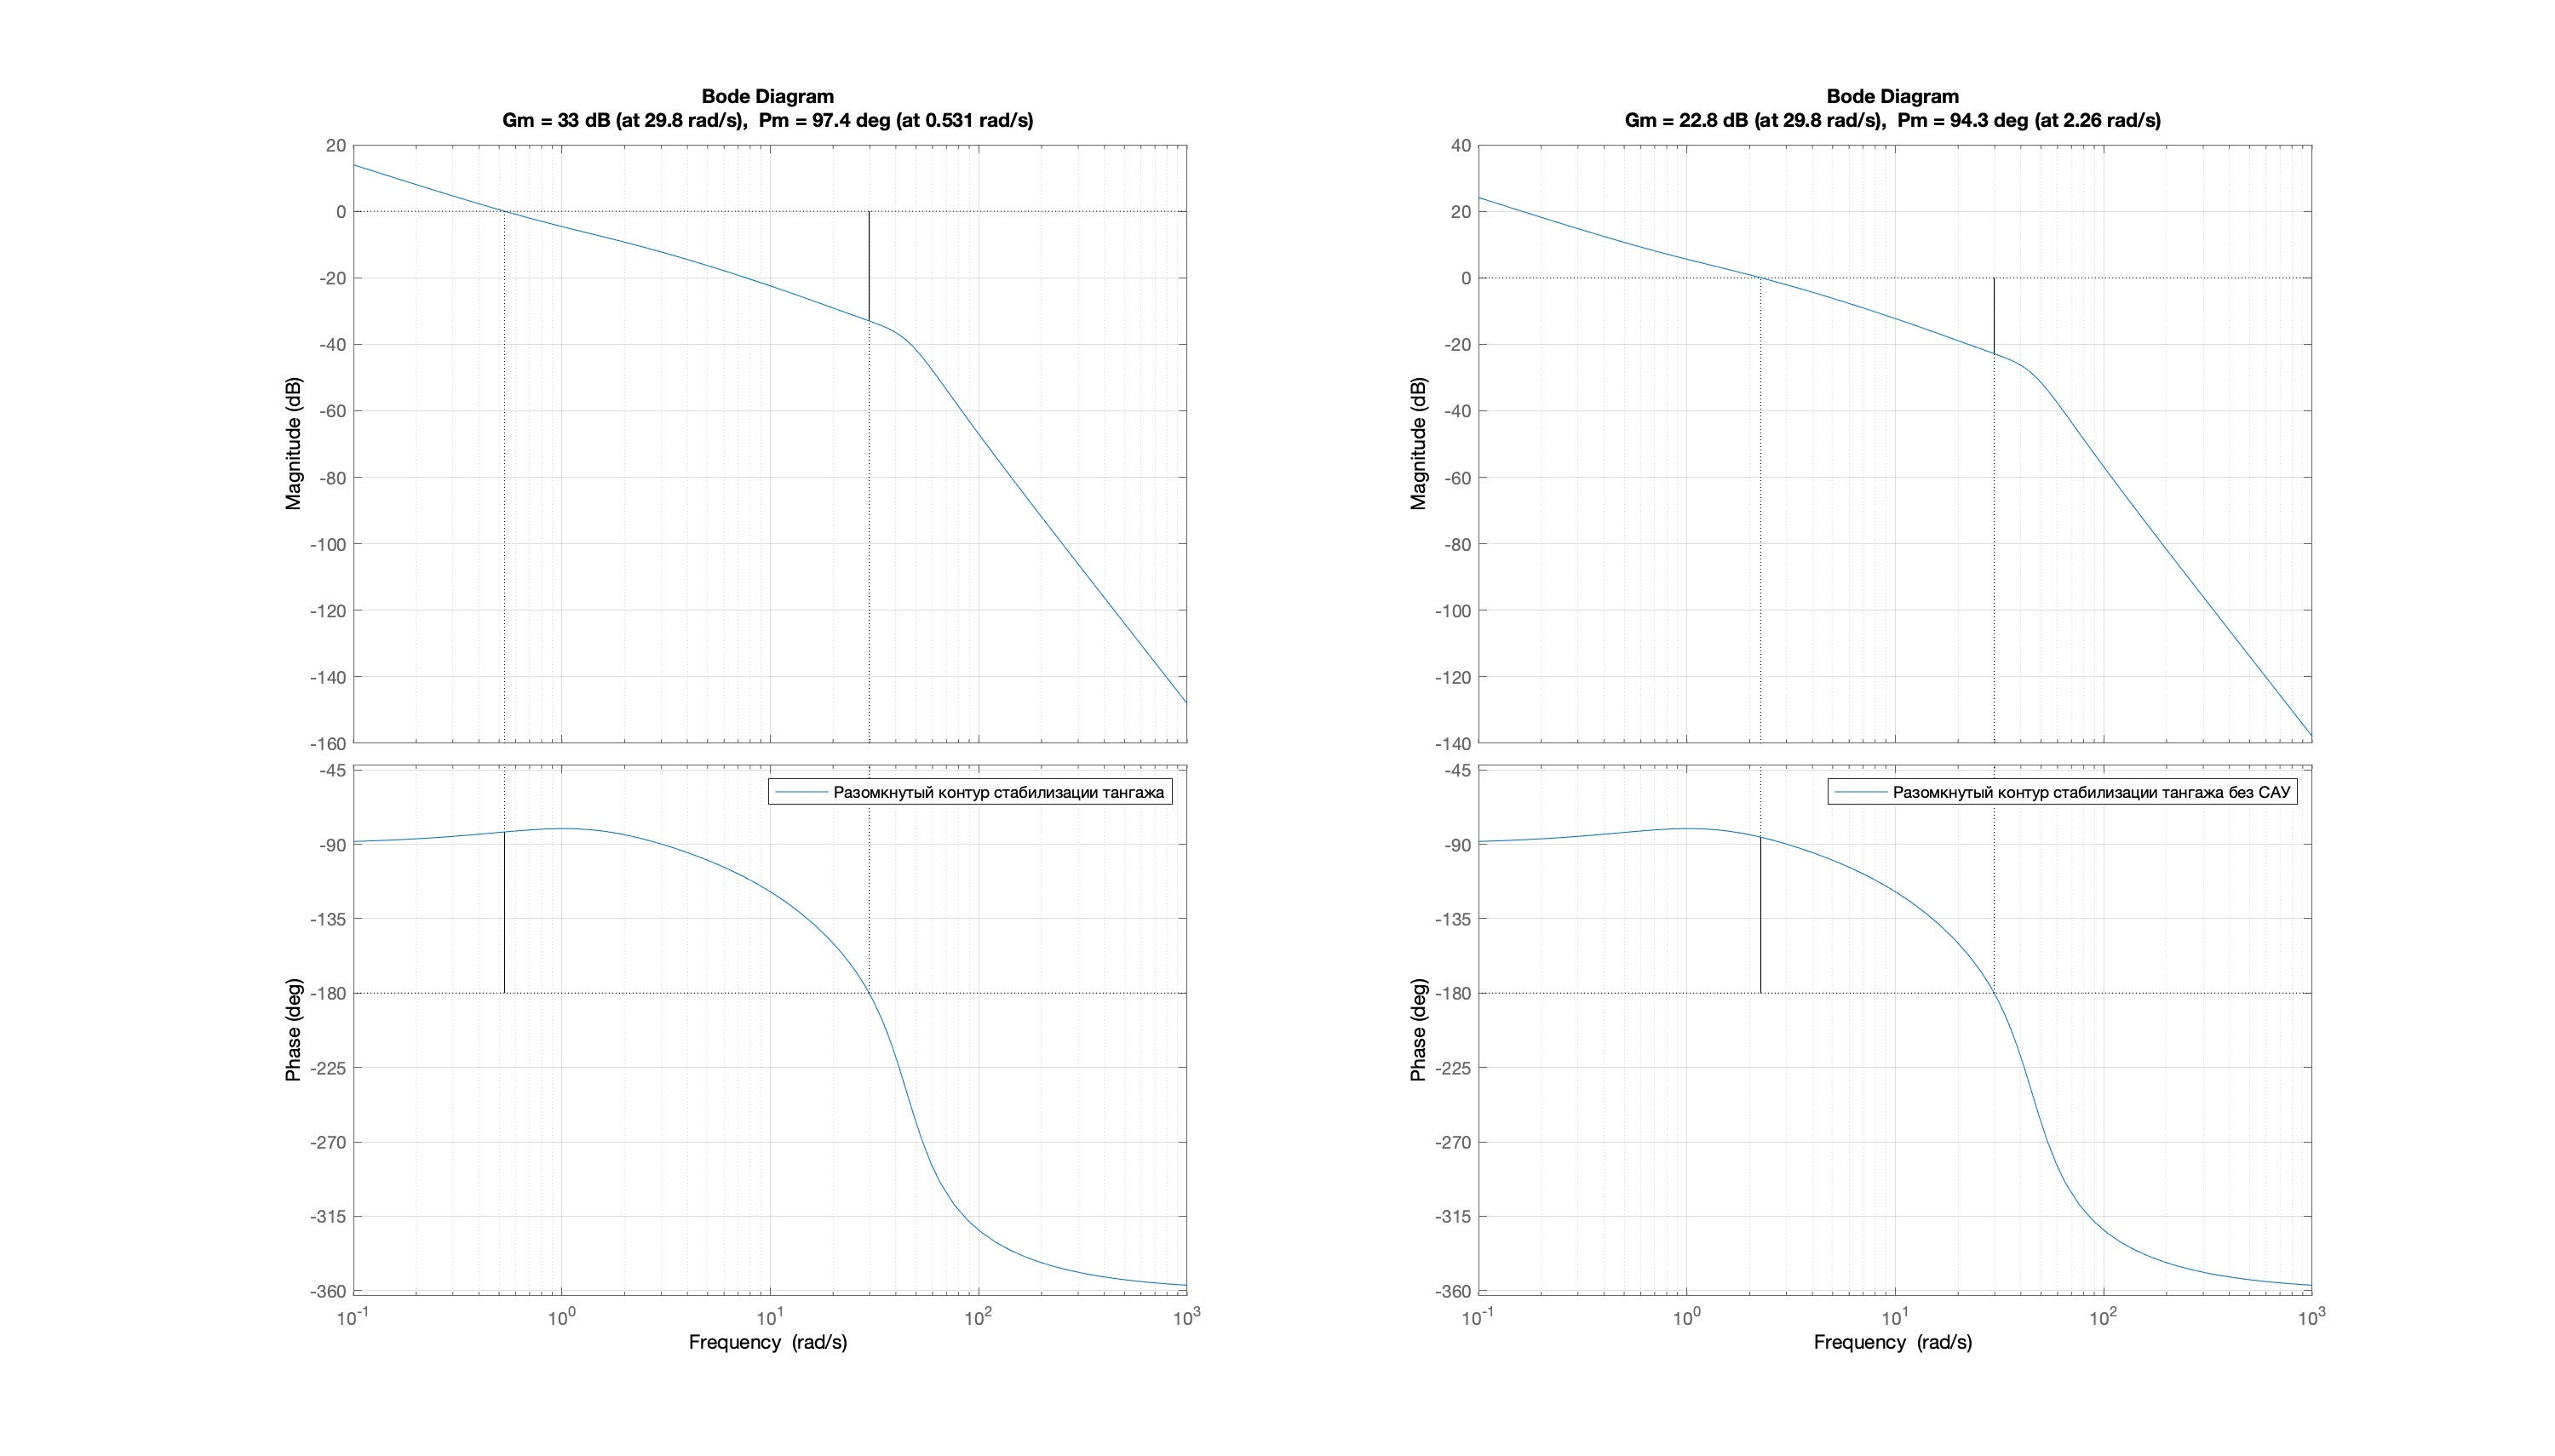
\includegraphics[width=\linewidth]{Оглавление/Part2/Sactions/Content/frequencies/Тангаж раз qMAX.jpg}}
    \caption{ЛАФЧХ разомкнутого контура стабилизации тангажа}
    \label{fig:Тангаж раз qMAX}
\end{figure}

Из рисунка \ref{fig:Тангаж раз qMAX} видно, что до синтеза данного контура запасы устойчивости по амплитуде и по фазе не удовлетворяют заданным требованиям, то есть запас по амплитуде меньше 10 дб и запас по фазе меньше 45 град, а после синтеза $\Delta A = 32,3 $дБ $\Delta \varphi = 95,9^0$, следовательно, синтез проведен успешно, коэффициенты рассчитаны верно. Замкнутая система будет устойчива.  

\begin{center}
    Контур вертикальной скорости:
\end{center}

\begin{figure}[H]
    \center{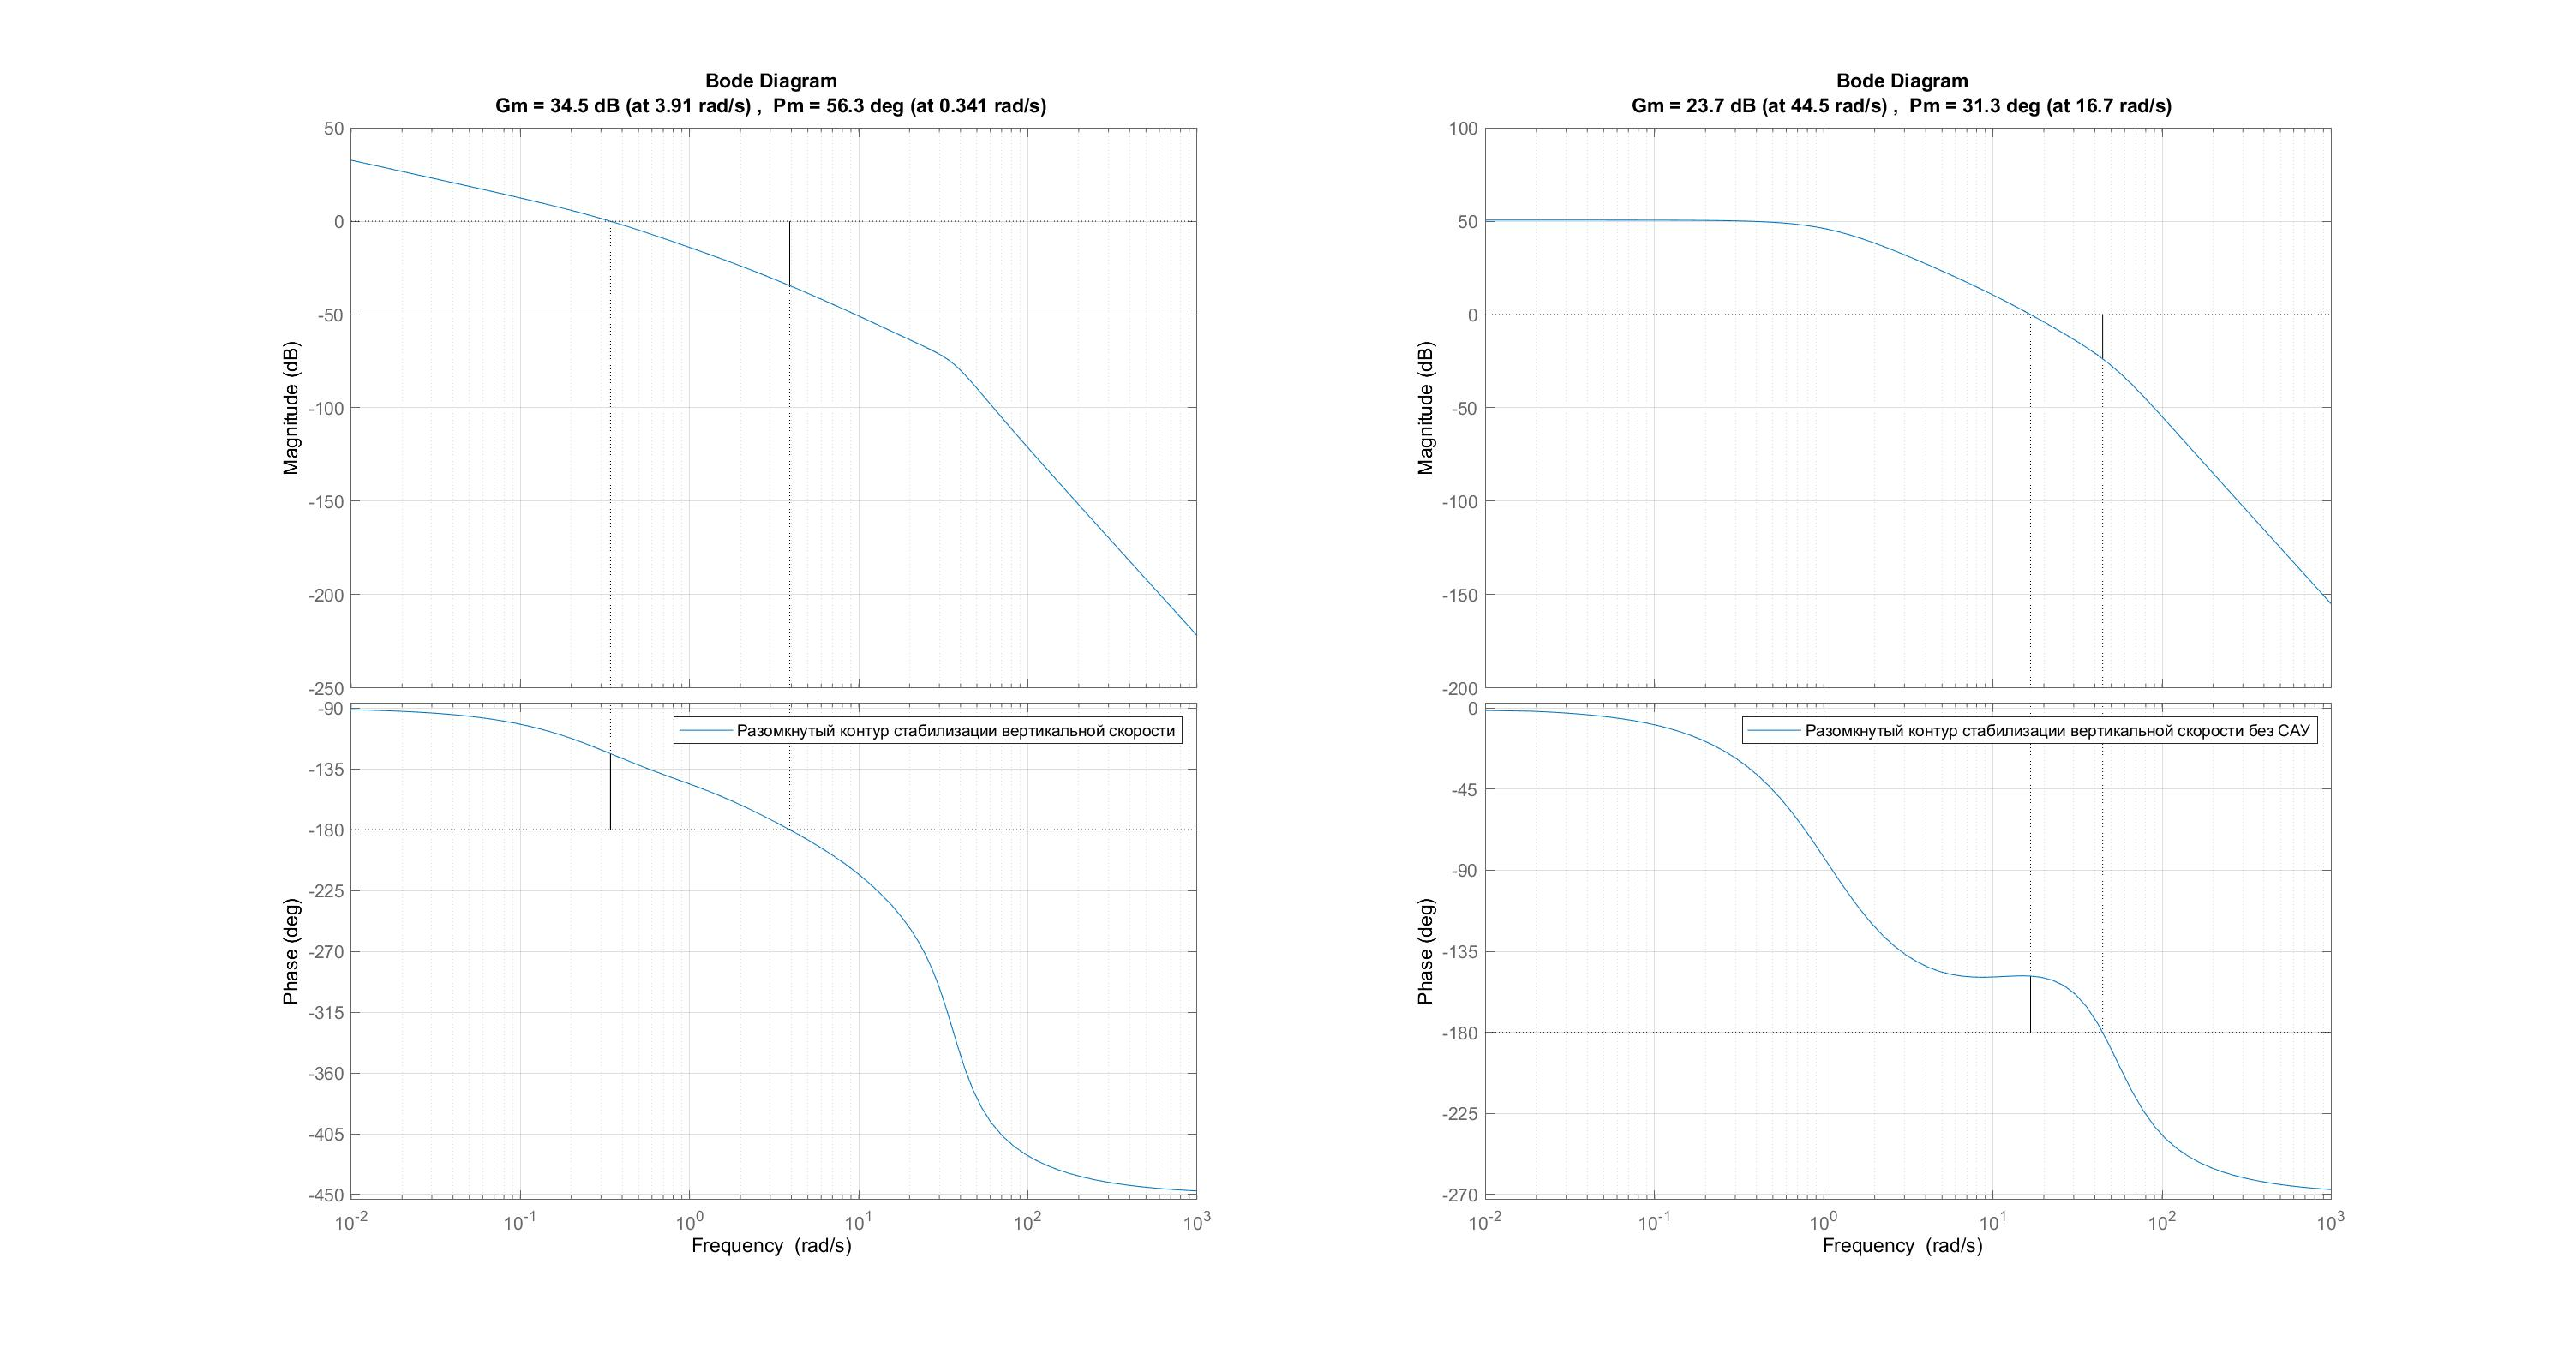
\includegraphics[width=\linewidth]{Оглавление/Part2/Sactions/Content/frequencies/Вертикальная скорость раз qMAX.jpg}}
    \caption{ЛАФЧХ разомкнутого контура стабилизации вертикальной скорости}
    \label{fig:Вертикальная скорость раз qMAX}
\end{figure}

Из рисунка \ref{fig:Вертикальная скорость раз qMAX} видно, что после синтеза $\Delta A = 34,5 $дБ $\Delta \varphi = 56,3^0$, следовательно, синтез проведен успешно, коэффициенты рассчитаны верно. Замкнутая система будет устойчива.  

\begin{figure}[H]
    \center{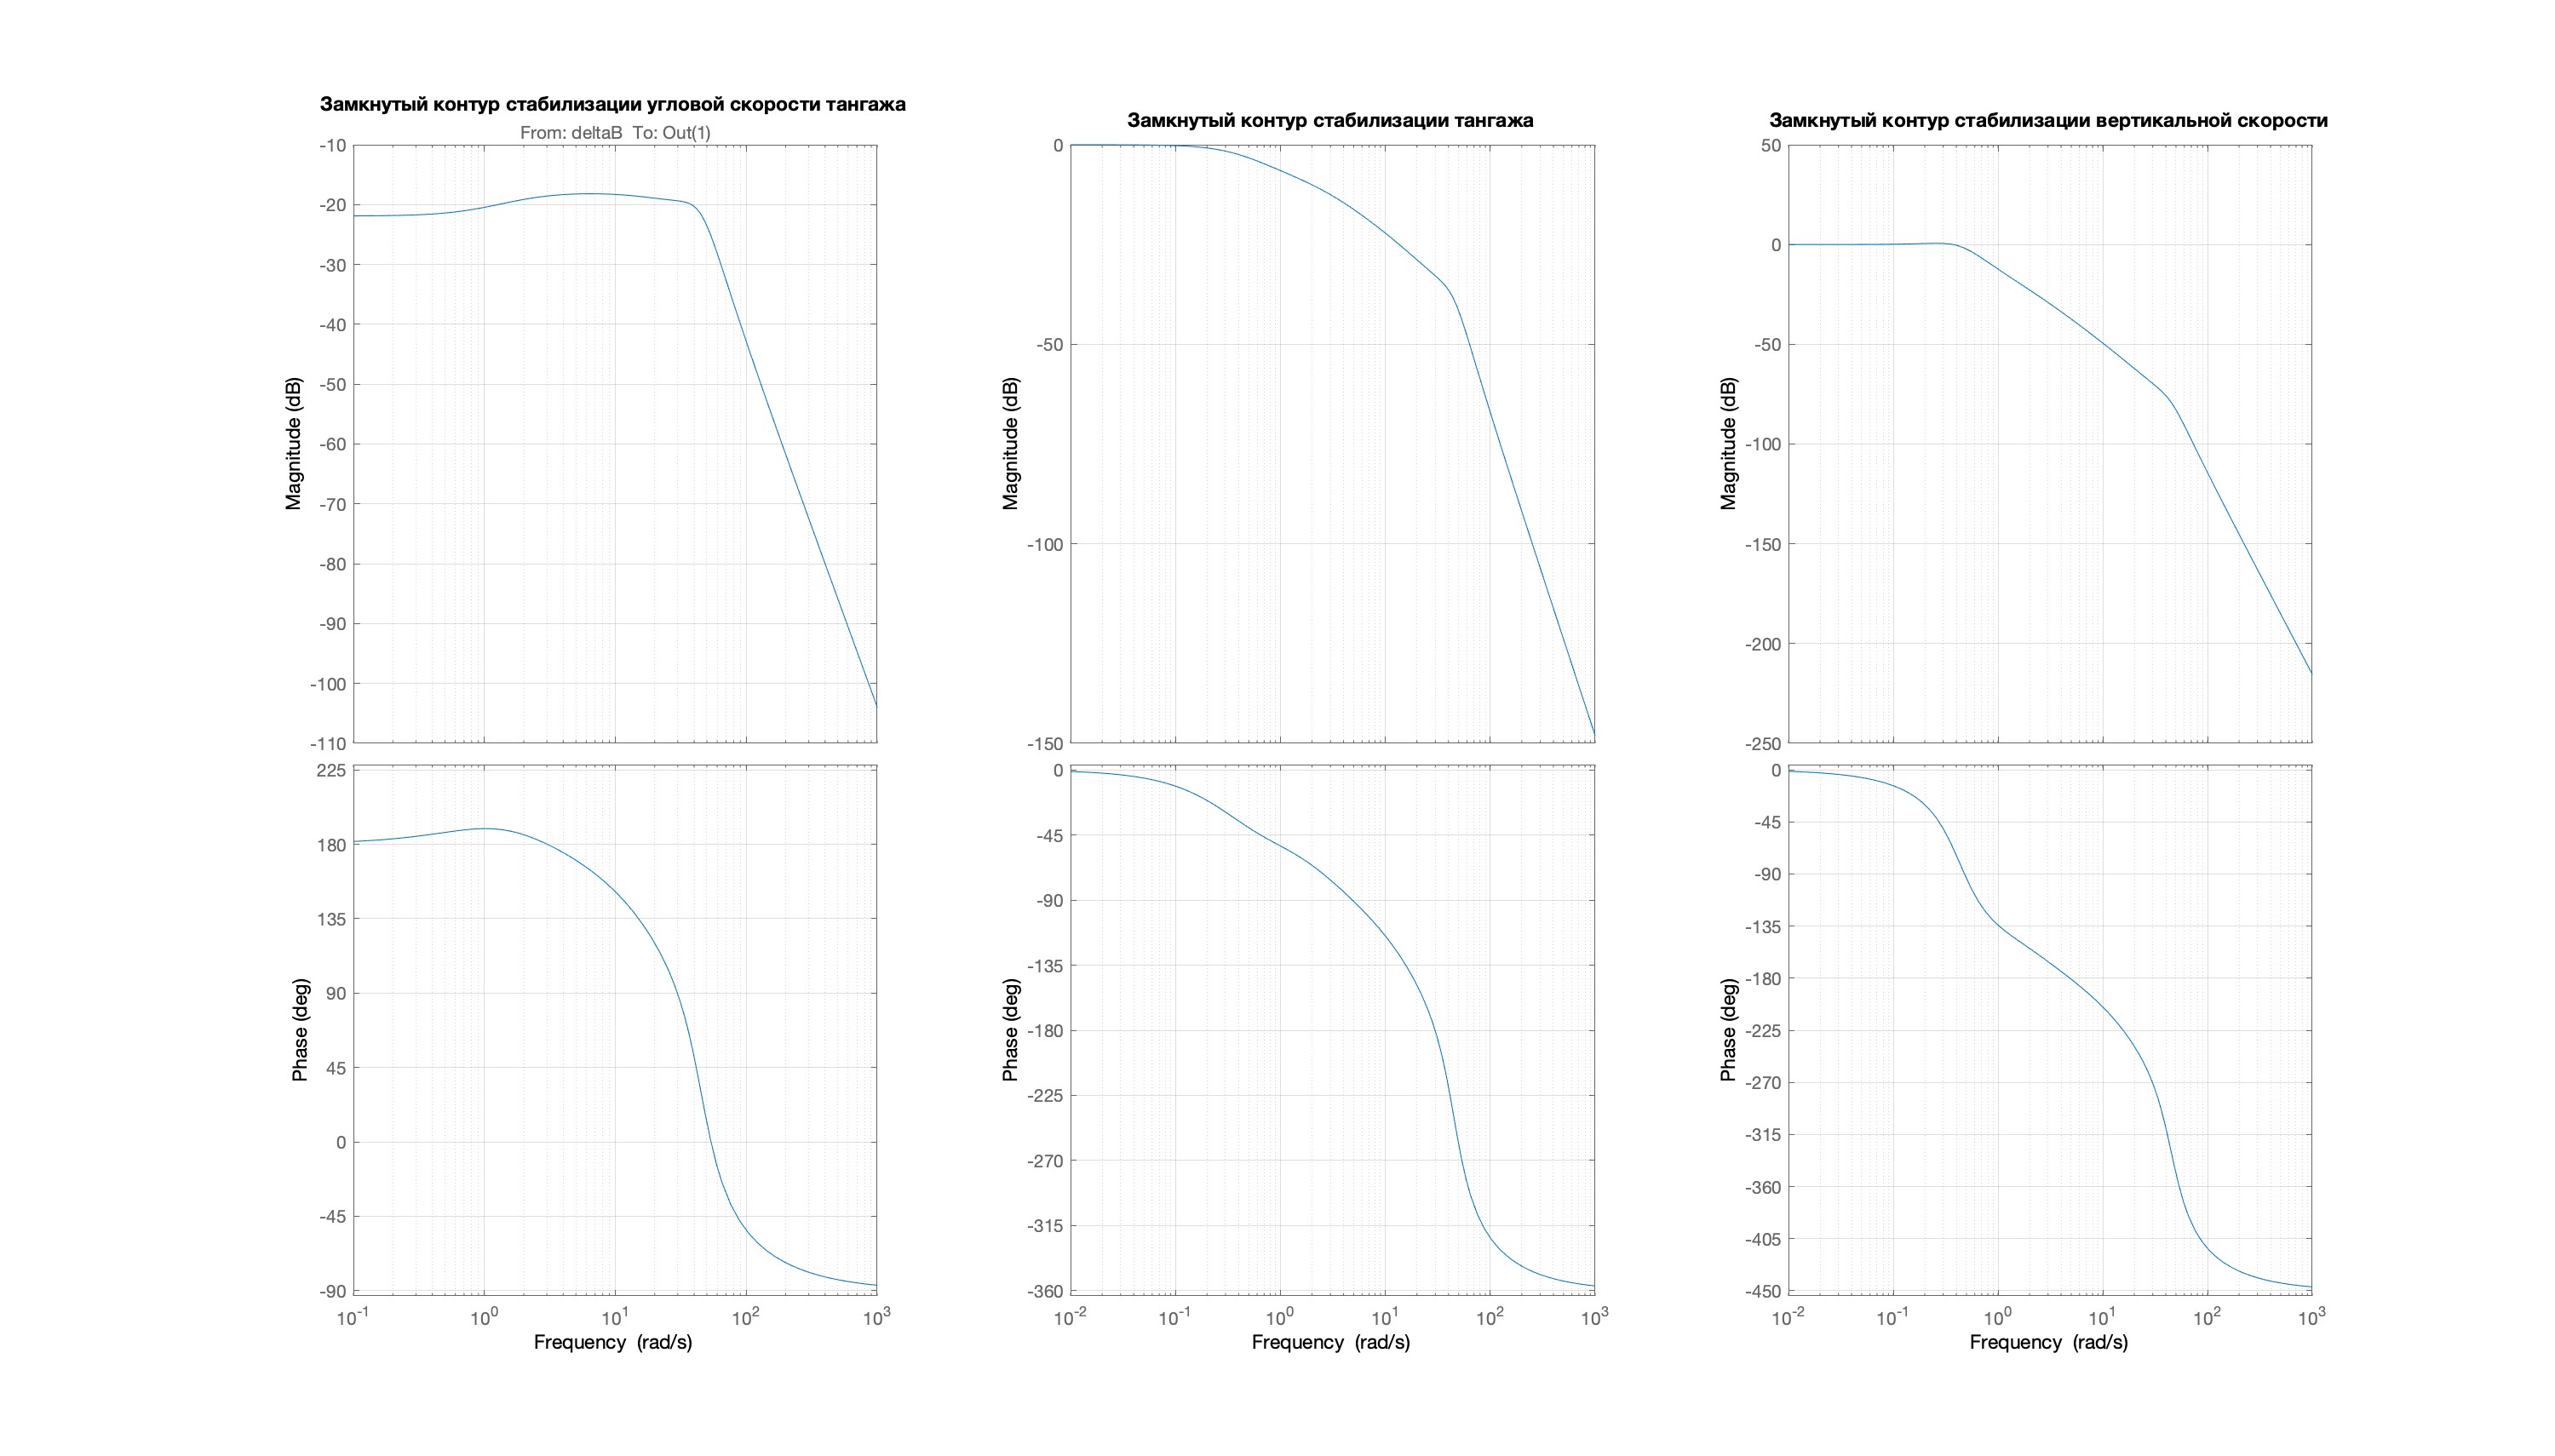
\includegraphics[width=\linewidth]{Оглавление/Part2/Sactions/Content/frequencies/ZAM qMAX.jpg}}
    \caption{ЛАФЧХ замкнутого контура }
    \label{fig:Вертикальная скорость зам qMAX}
\end{figure}

% __________________________________________________________________________________________
\subsubsubsection{Частотный анализ $q_{\text{кр}}$}

\begin{center}
    Контур демпфирования угловой скорости тангажа:
\end{center}

\begin{figure}[H]
    \center{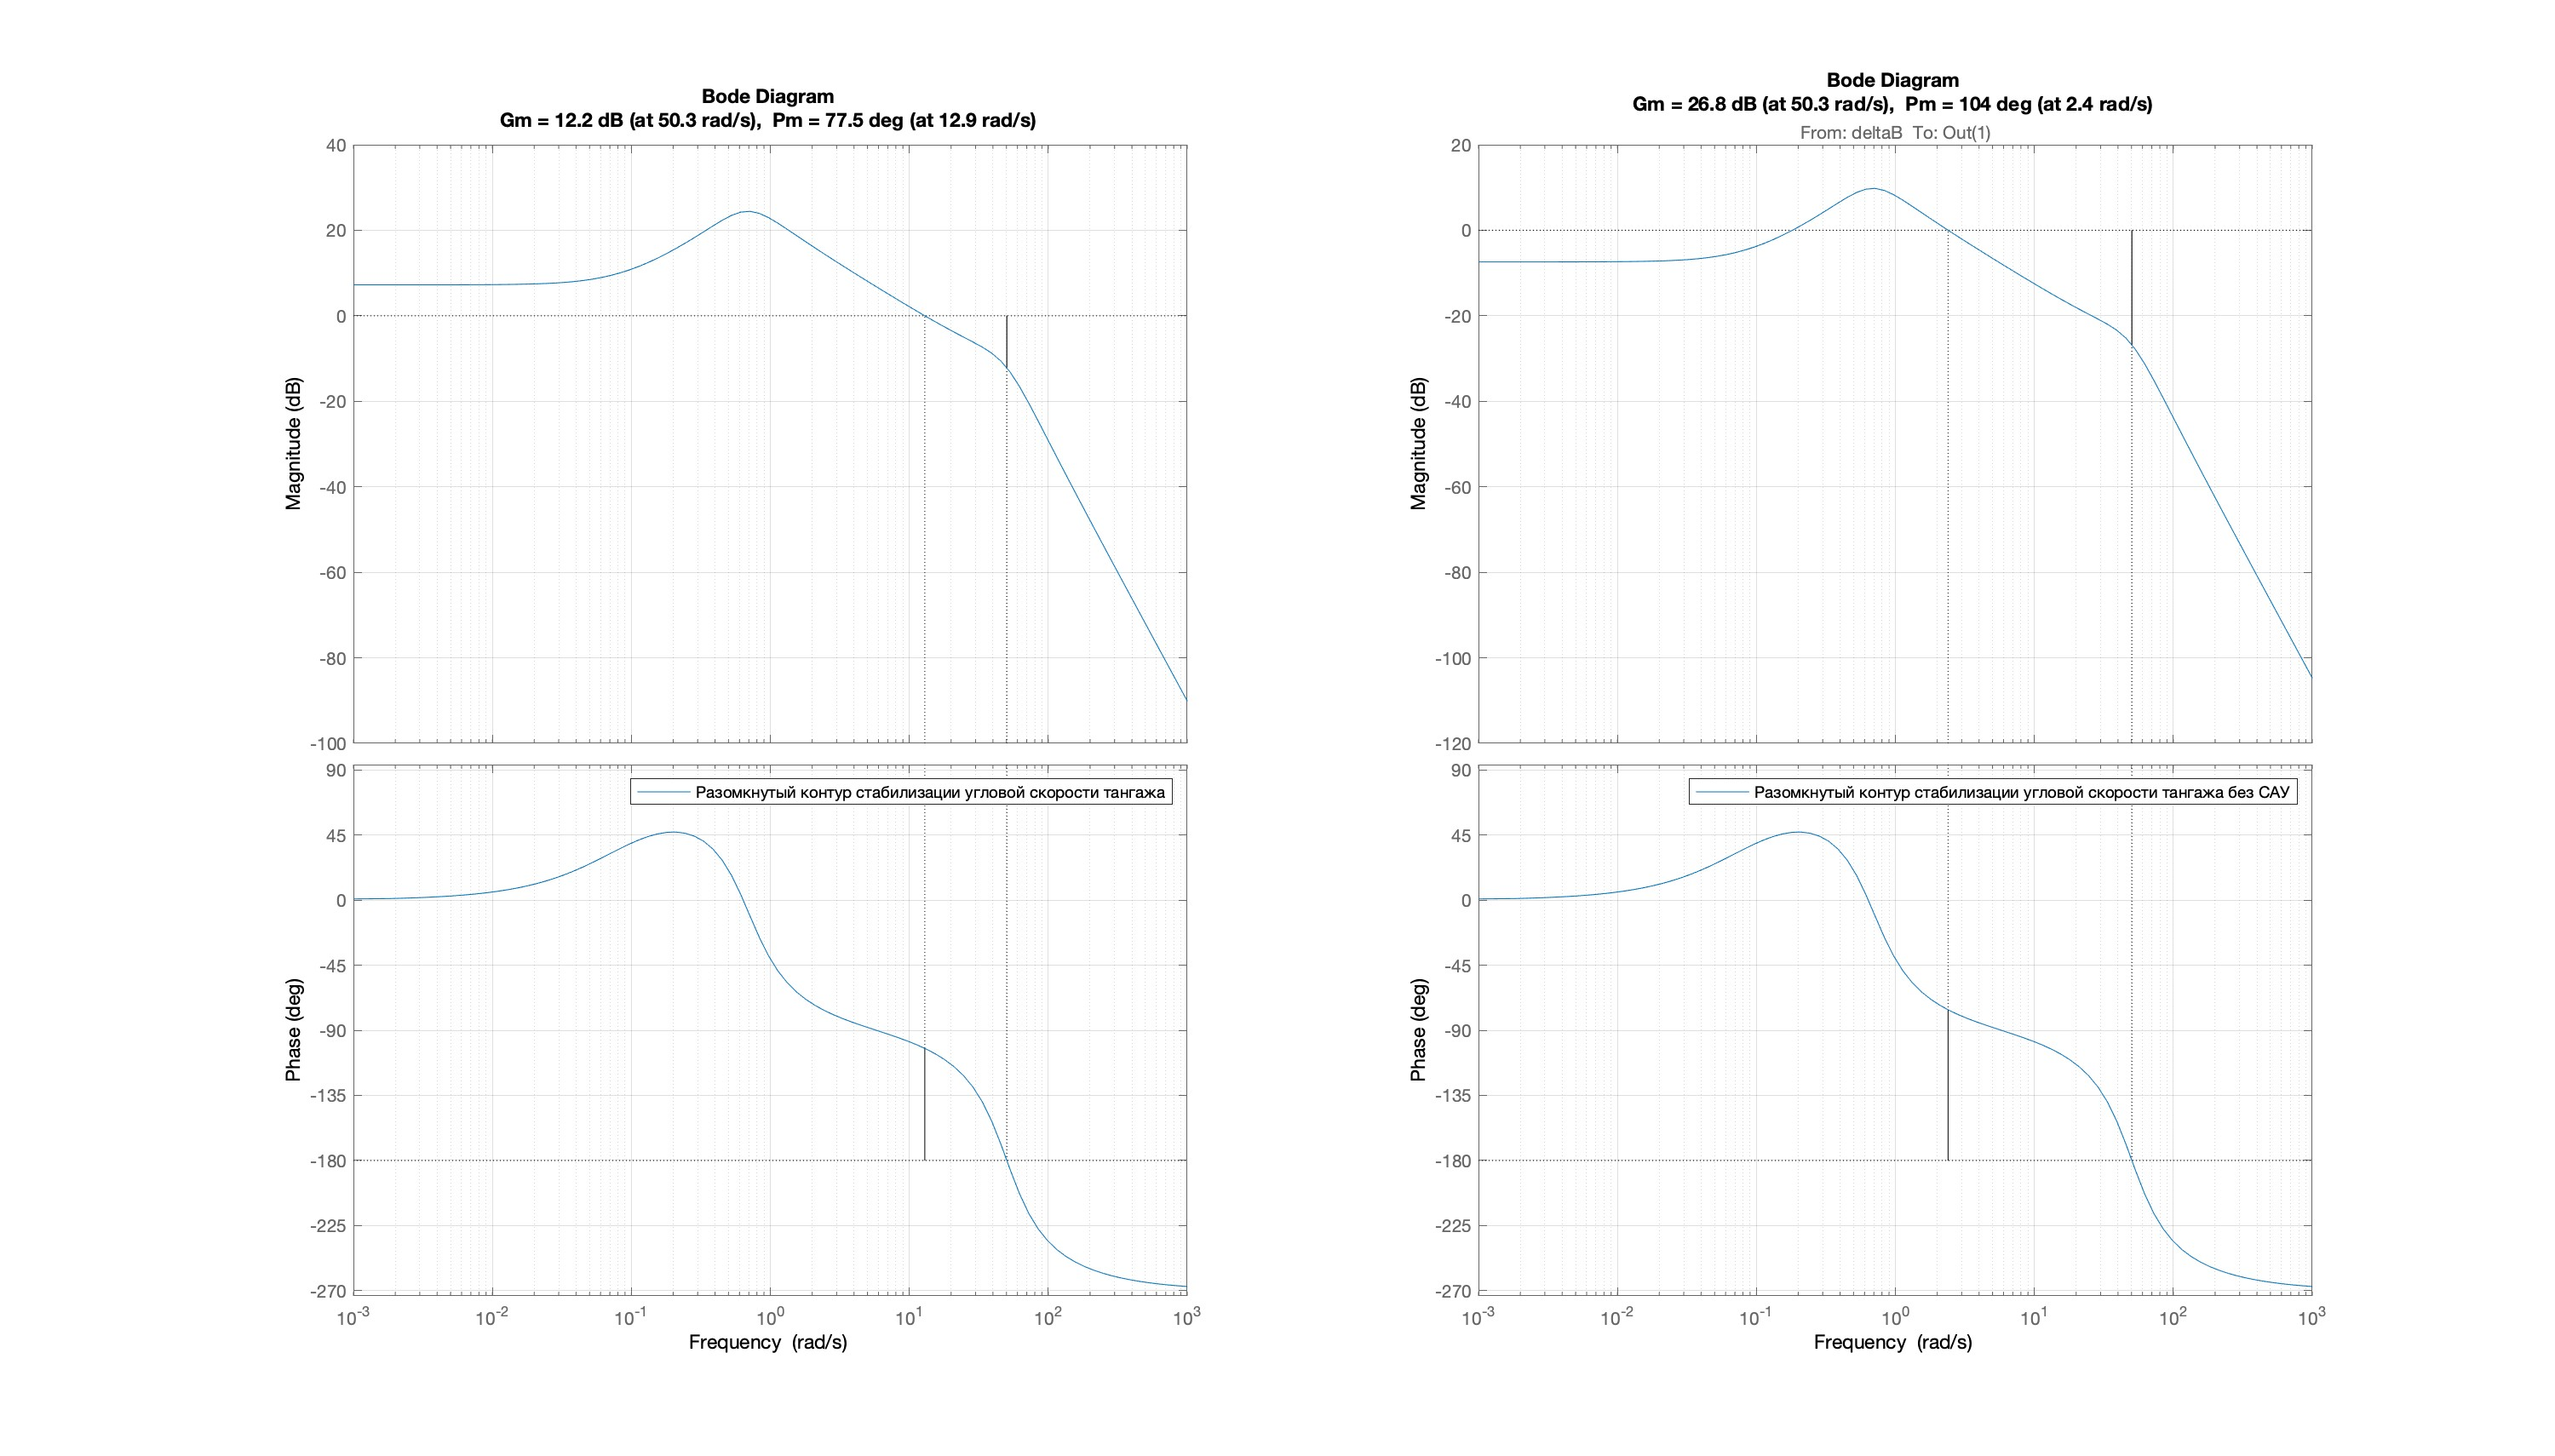
\includegraphics[width=\linewidth]{Оглавление/Part2/Sactions/Content/frequencies/Угловая скорость тангажа раз qKR.jpg}}
    \caption{ЛАФЧХ разомкнутого контура демпфирования угловой скорости тангажа}
    \label{fig:Угловая скорость тангажа раз qKR}
\end{figure}

Из рисунка \ref{fig:Угловая скорость тангажа раз qKR} видно, что до синтеза данного контура запасы устойчивости по амплитуде и по фазе не удовлетворяют заданным требованиям, то есть запас по амплитуде меньше 10 дб и запас по фазе меньше 45 град, а после синтеза $\Delta A = 12,3 $дБ $\Delta \varphi = 81^0$, следовательно, синтез проведен успешно, коэффициенты рассчитаны верно. Замкнутая система будет устойчива. Частота среза после синтеза не превысила граничного значения, она находится на участке с наклоном -20дб/дек, чего и требовалось достичь в результате синтеза.  

\begin{center}
    Контур стабилизации тангажа:
\end{center}

\begin{figure}[H]
    \center{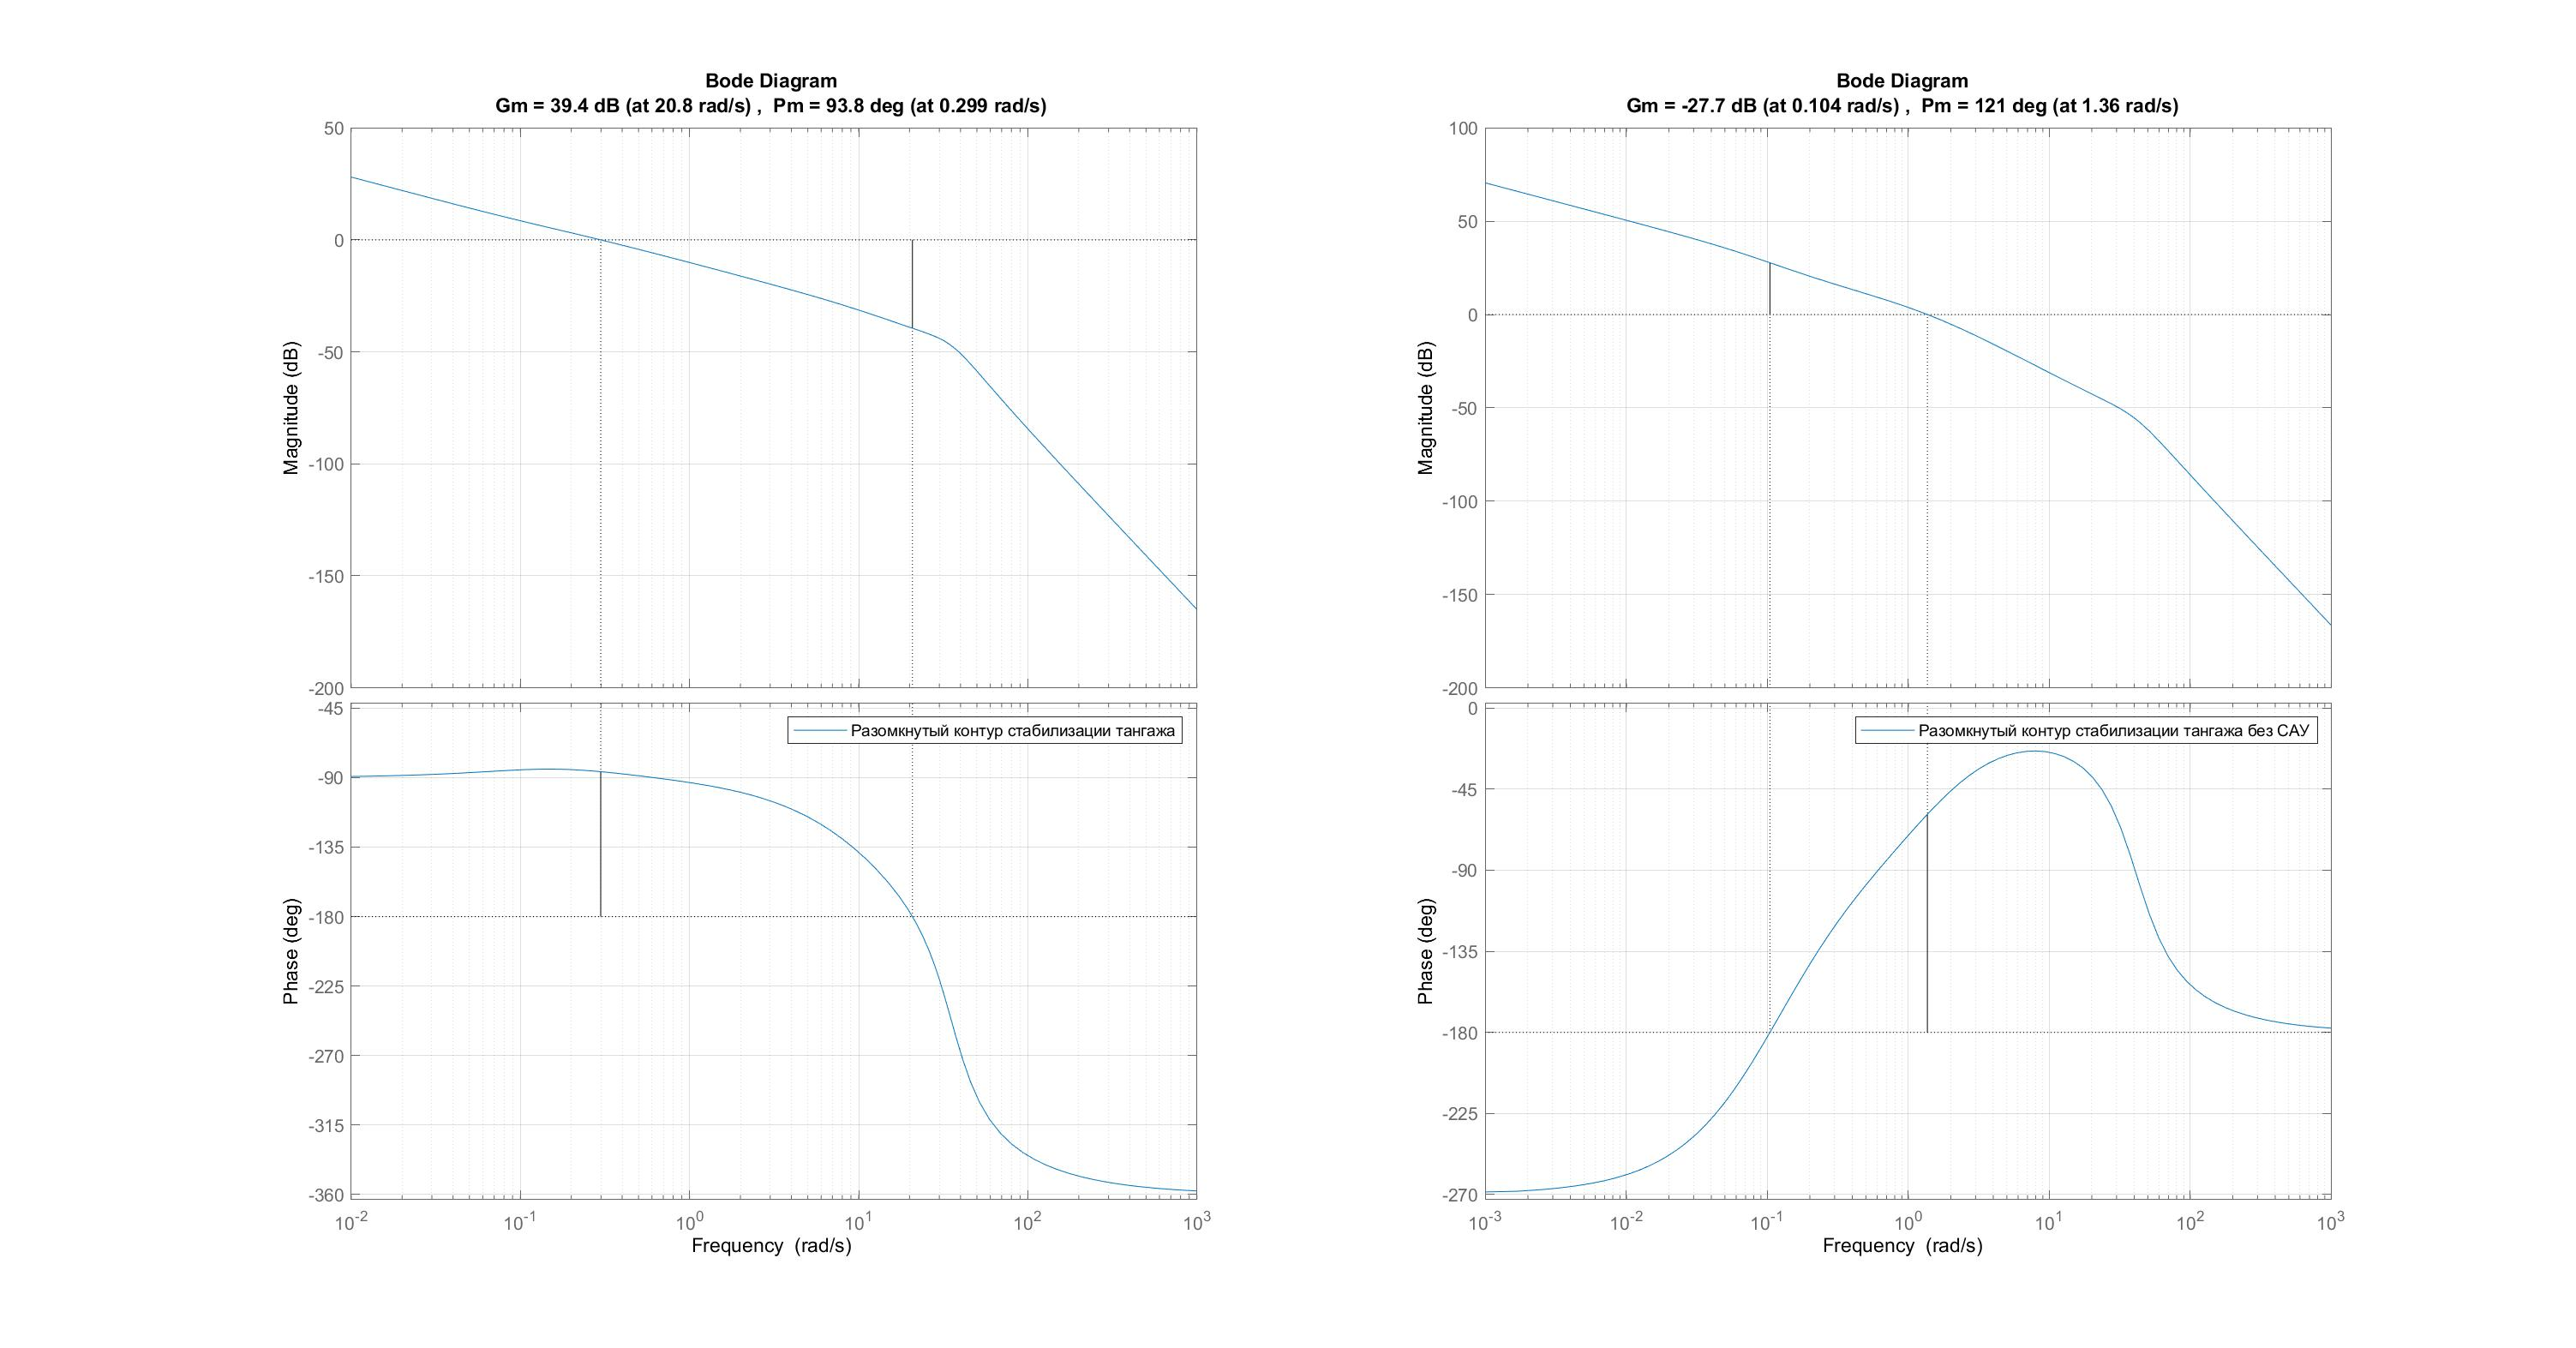
\includegraphics[width=\linewidth]{Оглавление/Part2/Sactions/Content/frequencies/Тангаж раз qKR.jpg}}
    \caption{ЛАФЧХ разомкнутого контура стабилизации тангажа}
    \label{fig:Тангаж раз qKR}
\end{figure}

Из рисунка \ref{fig:Тангаж раз qKR} видно, что до синтеза данного контура запасы устойчивости по амплитуде и по фазе не удовлетворяют заданным требованиям, то есть запас по амплитуде меньше 10 дб и запас по фазе меньше 45 град, а после синтеза $\Delta A = 39,4 $дБ $\Delta \varphi = 94^0$, следовательно, синтез проведен успешно, коэффициенты рассчитаны верно. Замкнутая система будет устойчива.  

\begin{center}
    Контур вертикальной скорости:
\end{center}

\begin{figure}[H]
    \center{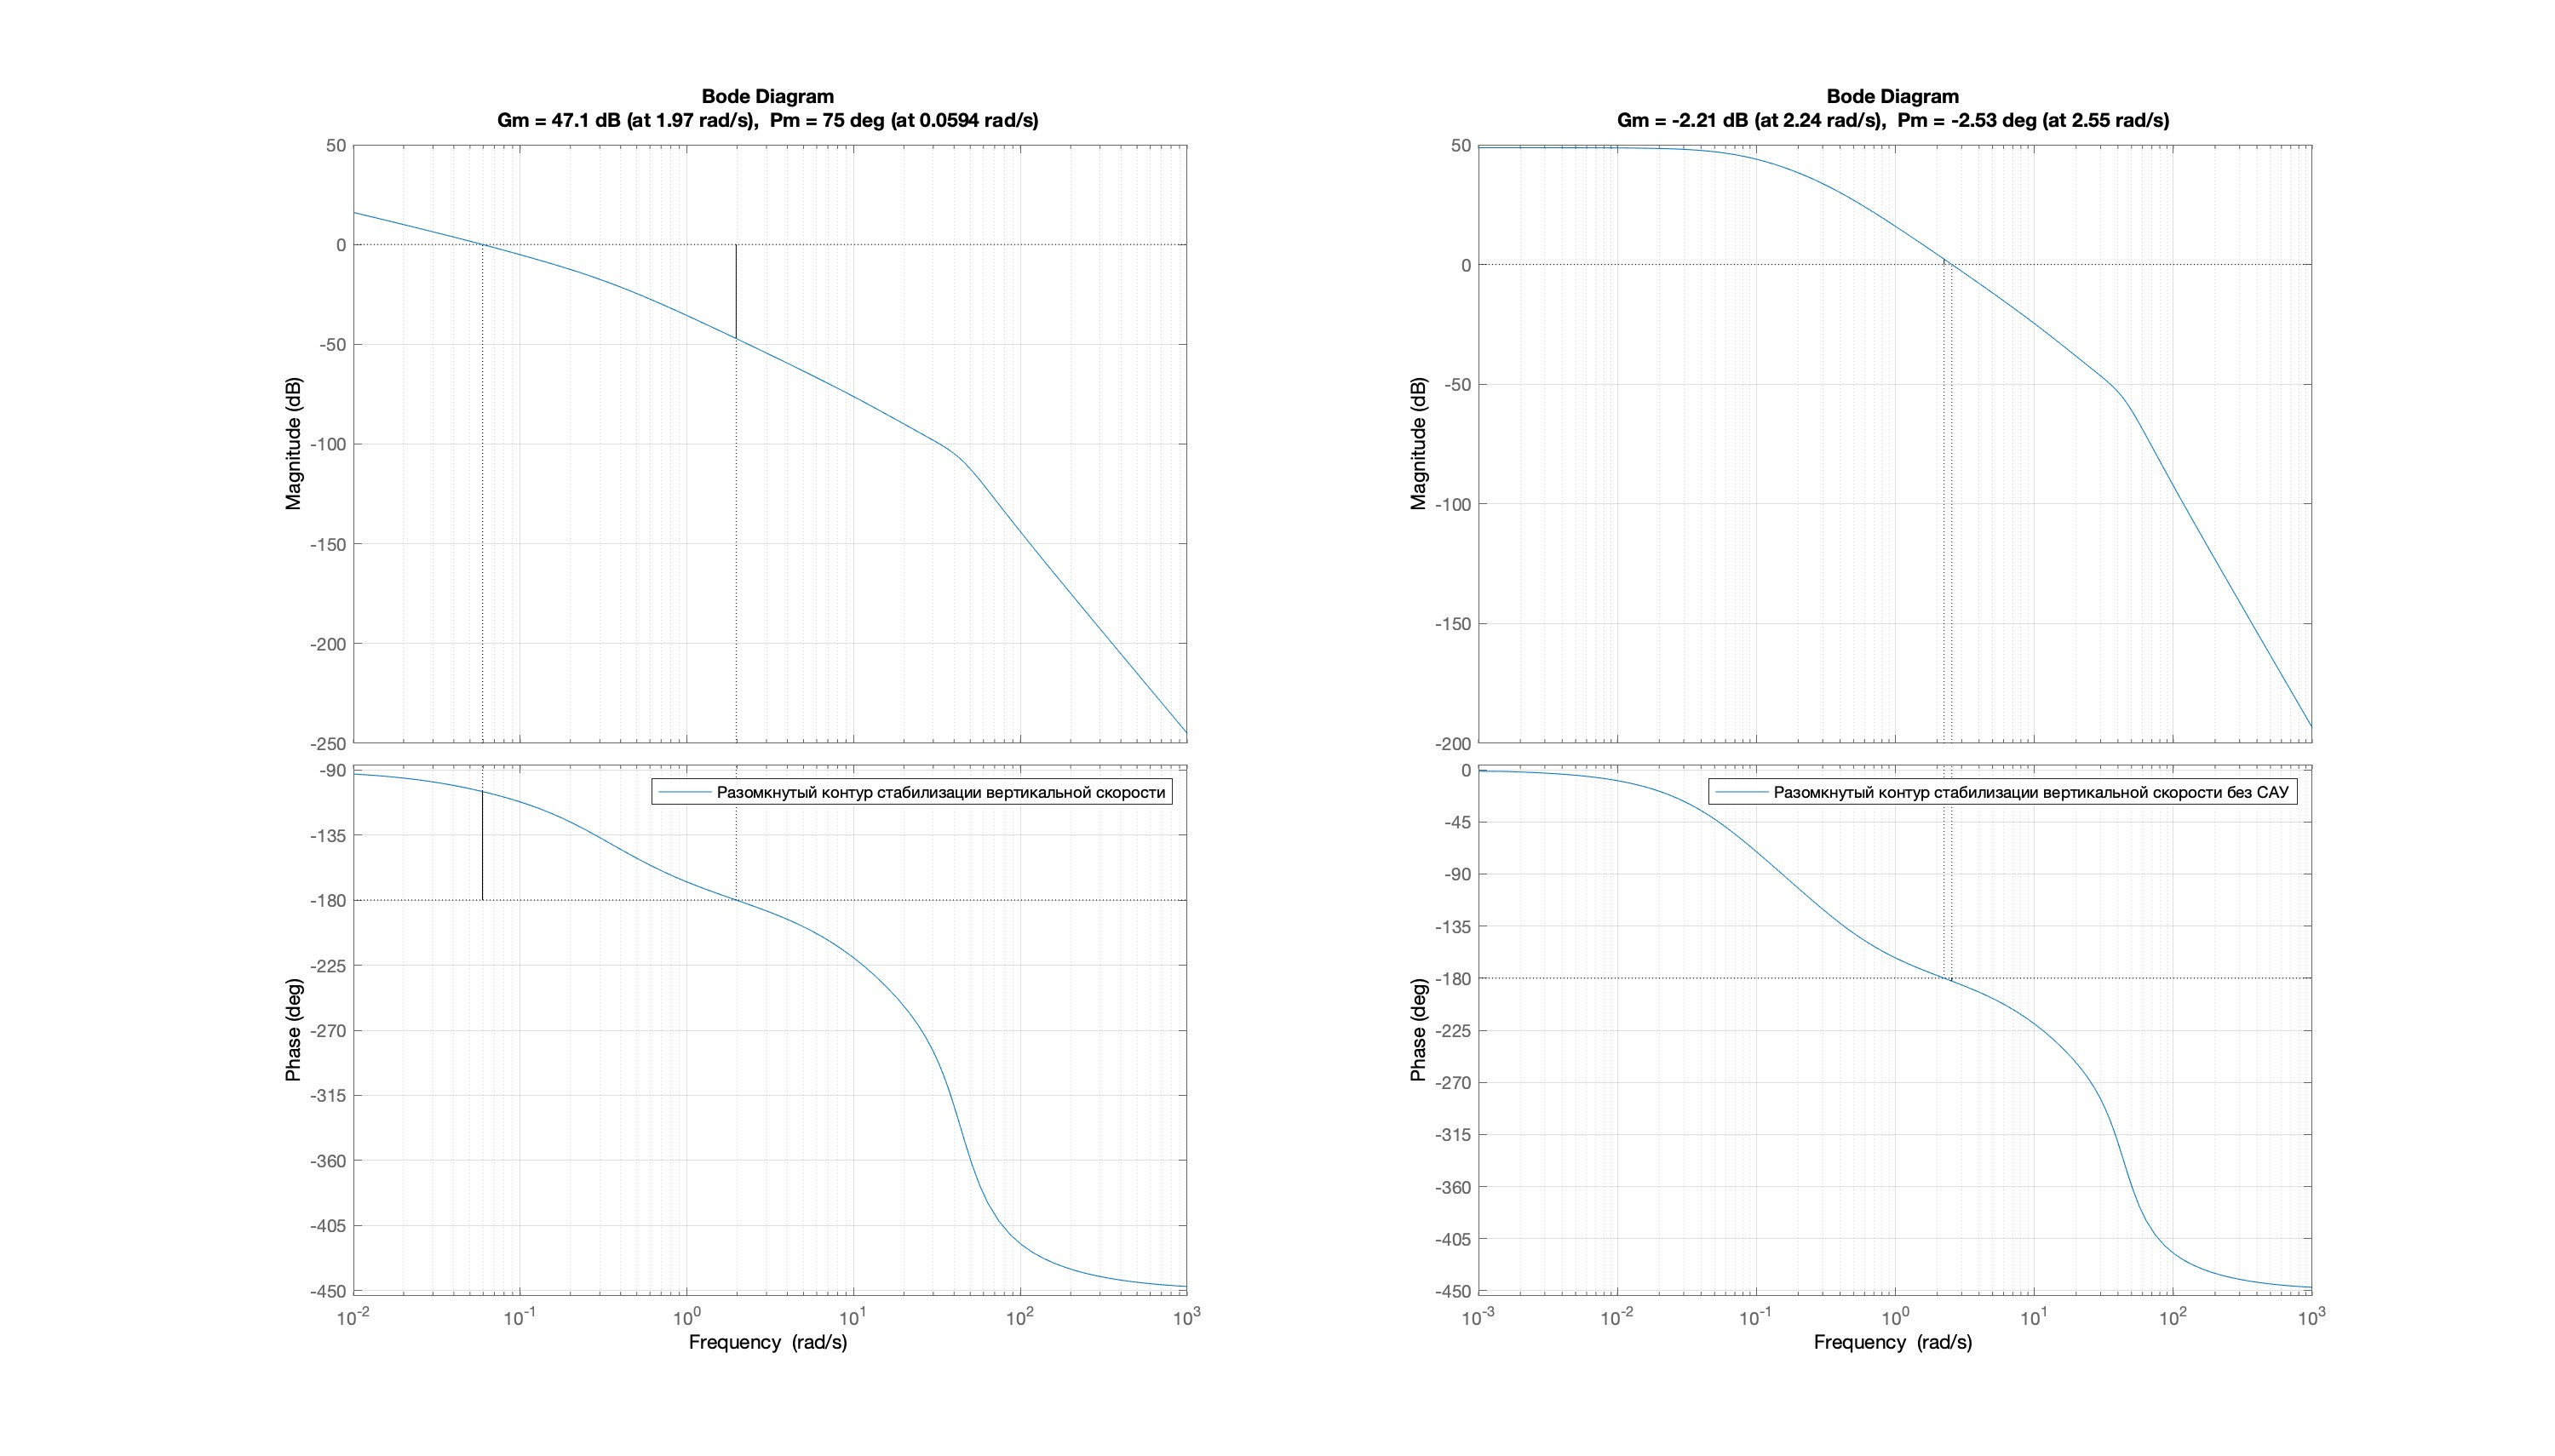
\includegraphics[width=\linewidth]{Оглавление/Part2/Sactions/Content/frequencies/Вертикальная скорость раз qKR.jpg}}
    \caption{ЛАФЧХ разомкнутого контура стабилизации вертикальной скорости}
    \label{fig:Вертикальная скорость раз qKR}
\end{figure}

Из рисунка \ref{fig:Вертикальная скорость раз qKR} видно, что после синтеза $\Delta A = 41,9 $дБ $\Delta \varphi = 72^0$, следовательно, синтез проведен успешно, коэффициенты рассчитаны верно. Замкнутая система будет устойчива.  

\begin{figure}[H]
    \center{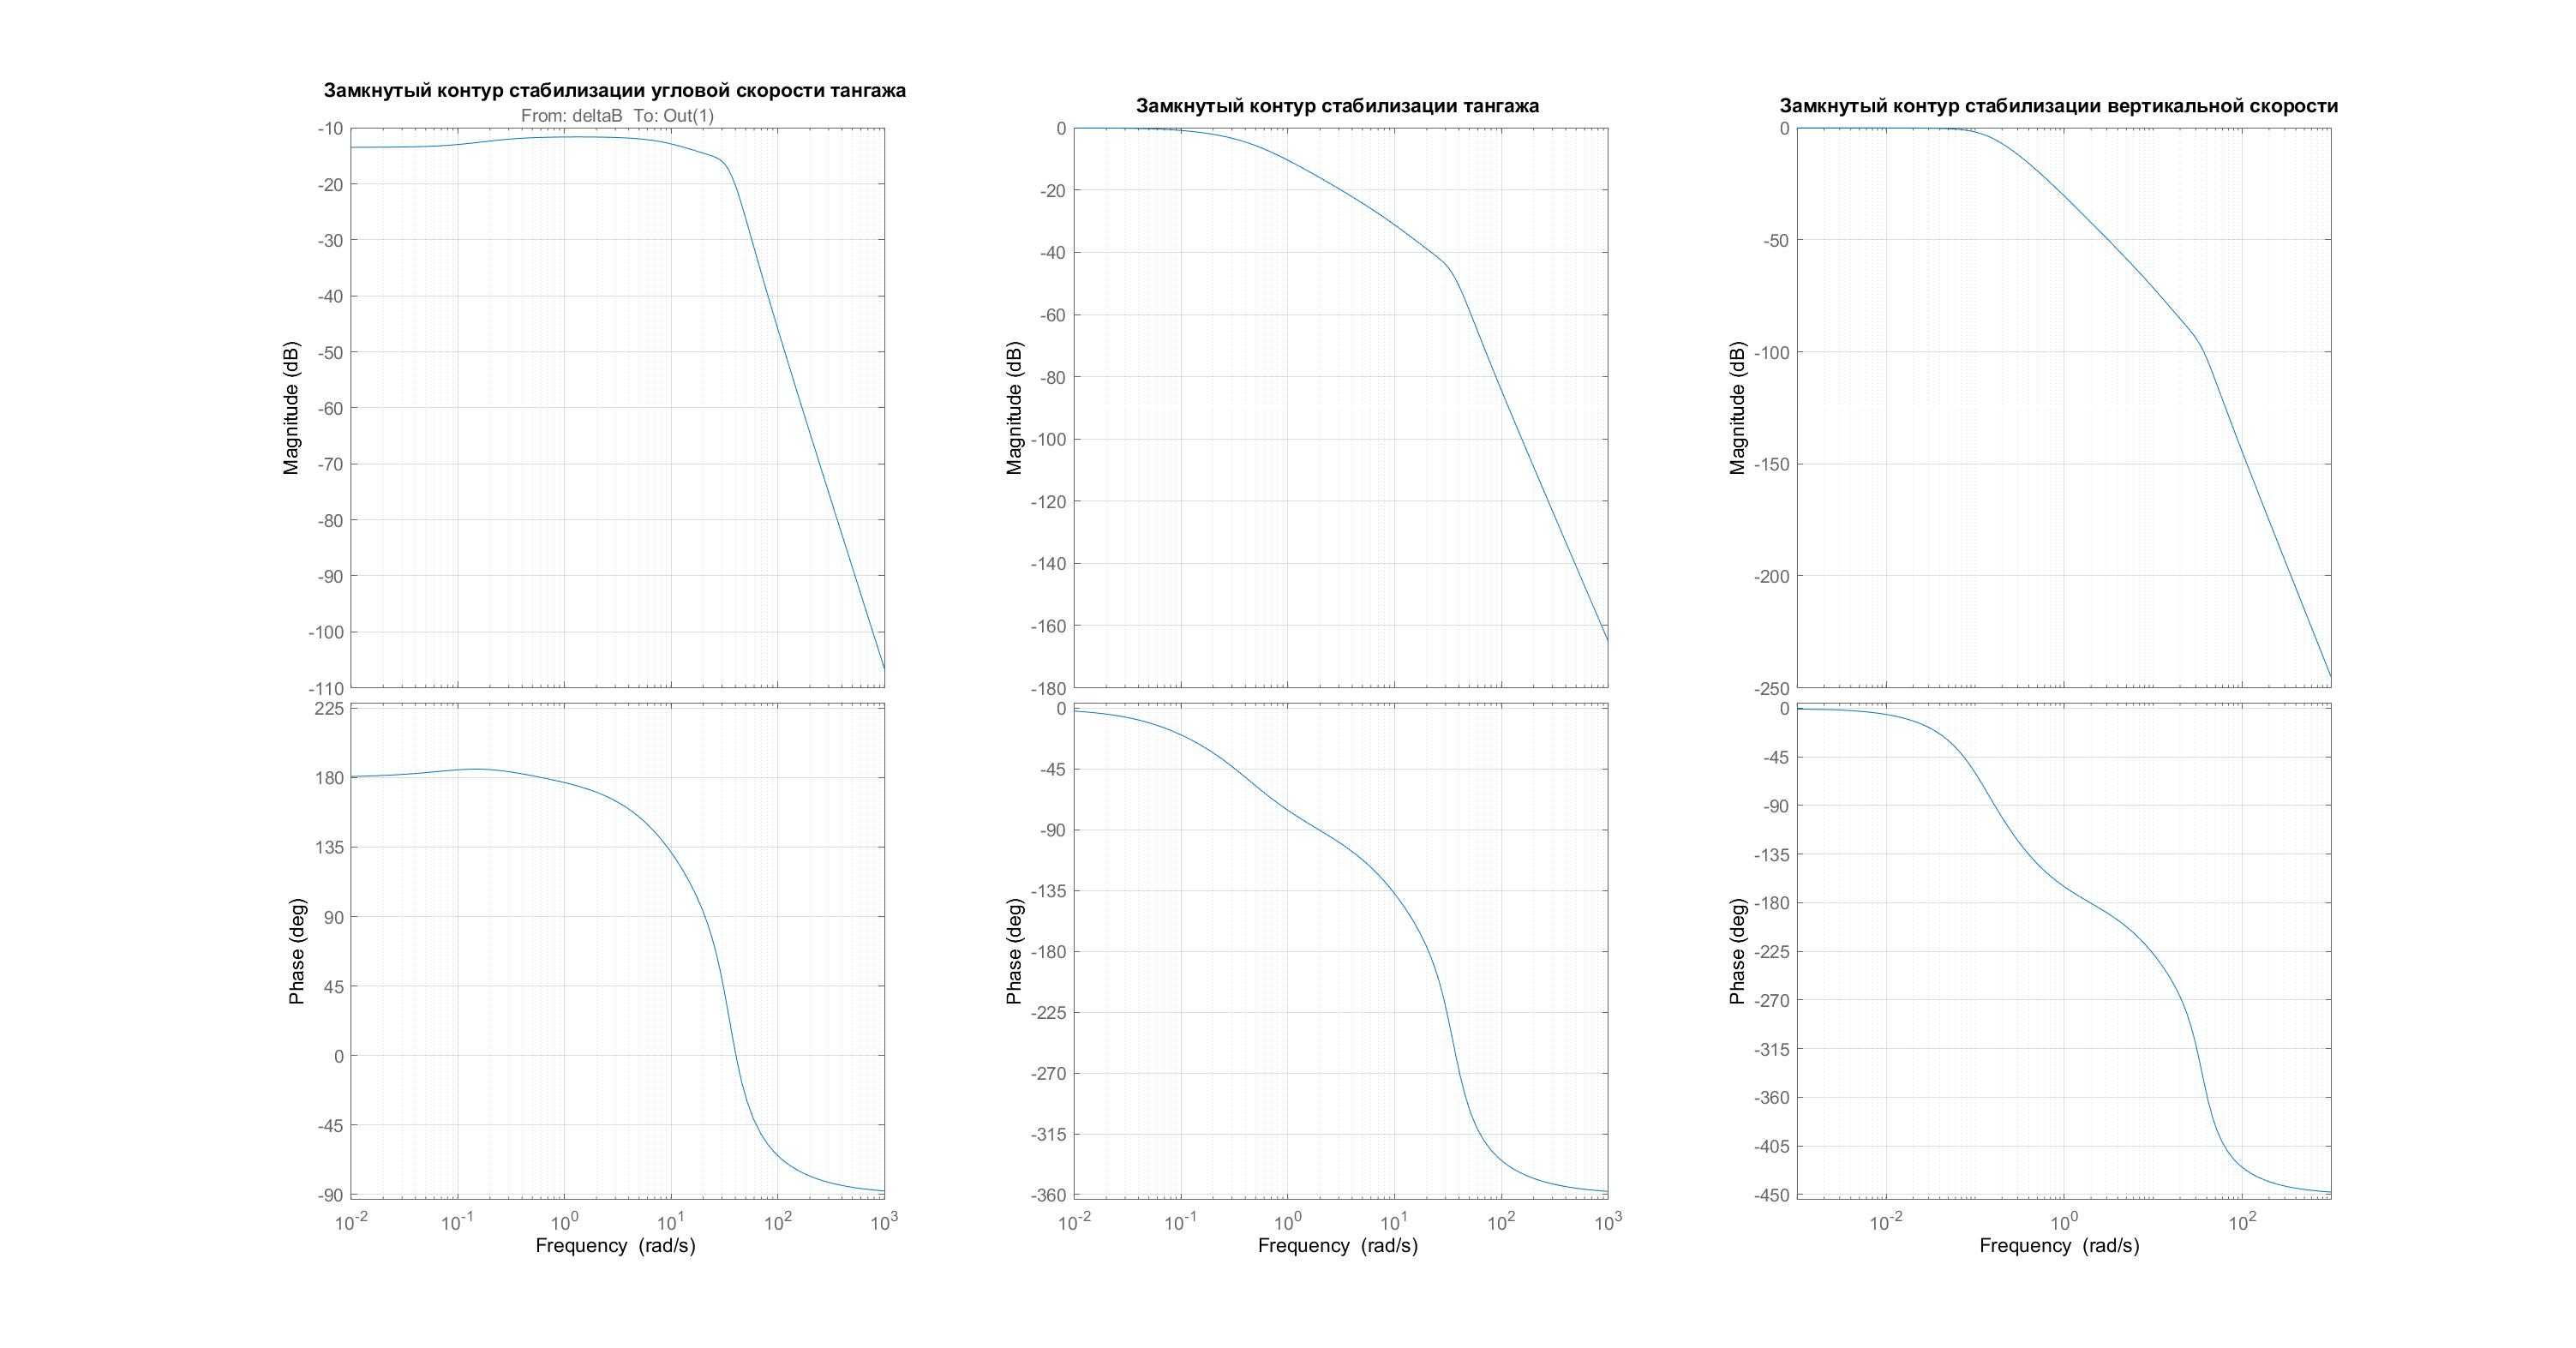
\includegraphics[width=\linewidth]{Оглавление/Part2/Sactions/Content/frequencies/ZAM qKR.jpg}}
    \caption{ЛАФЧХ замкнутого контура }
    \label{fig:Вертикальная скорость зам qKR}
\end{figure}

\subsection{Нелинейное моделирование САУ}

В данном разделе проводится анализ линейной и нелинейной САУ. В Simulink реализуется система управления на крейсерском режиме полета. Крейсерскому режиму полета для самолета-прототипа Concorde соответствуют М=0,7521 и Н=10 км. Найденные коэффициенты для данного режима полета приведены в таблице 2.9 раздела 2. 

В системе появляется нелинейность из-за введения ограничений по углу тангажа, скорости изменения сигнала, поступающего на привод и т.д. В Simulink ограничения можно ввести при помощи блоков «Saturation» и «Rate limiter». Величины ограничений приведены в таблице \ref{tab:Нелинейности}

\begin{table}[H]
    \centering
    \caption{ограничения, вводимые в САУ}
    \begin{tabular}{|c|c|c|c|c|}
    \hline
        № & Параметр & Обозначение & Значение & Единица измерения \\ \hline
        1 & Максимальный угол & $\delta_\text{э}_\text{макс}$ & $\pm 25$ & град \\ 
         & отклонения элевонов &  &  & \\ \hline
        2 & Максимальный угол & $\vartheta_\text{макс}$ & $\pm 23$ & град\\
         & тангажа &  &  & \\ \hline
         & Скорость изменения &  &  & \\ 
        3 & сигнала на & $\dot{\sigma_n}$ & $\pm 30$ &ед \\ 
        & выходе в привод &  &  & \\ \hline
        4 & Величина входного &  &  & \\ 
         & сигнала привода & $\sigma_n$ & $\pm 15$ &ед \\ \hline
    \end{tabular}
    \label{tab:Нелинейности}
\end{table}

Моделирование нелинейной системы проводится при стабилизации вертикальной скорости $V_y = 10$м/с, моделирование линейной при стабилизации угла курса  .Результаты линейного и нелинейного моделирования представлены в виде графиков различных переходных процессов (см. рис.3.1-3.18). Схема системы представлена в конце данного раздела.

\begin{center}
    \subsubsection{Моделирование линейной и нелинейной САУ}Моделирование линейной и нелинейной САУ
\end{center}

Структурные схемы линейной и нелинейной системы представлены в приложениях.

\begin{figure}[H]
    \center{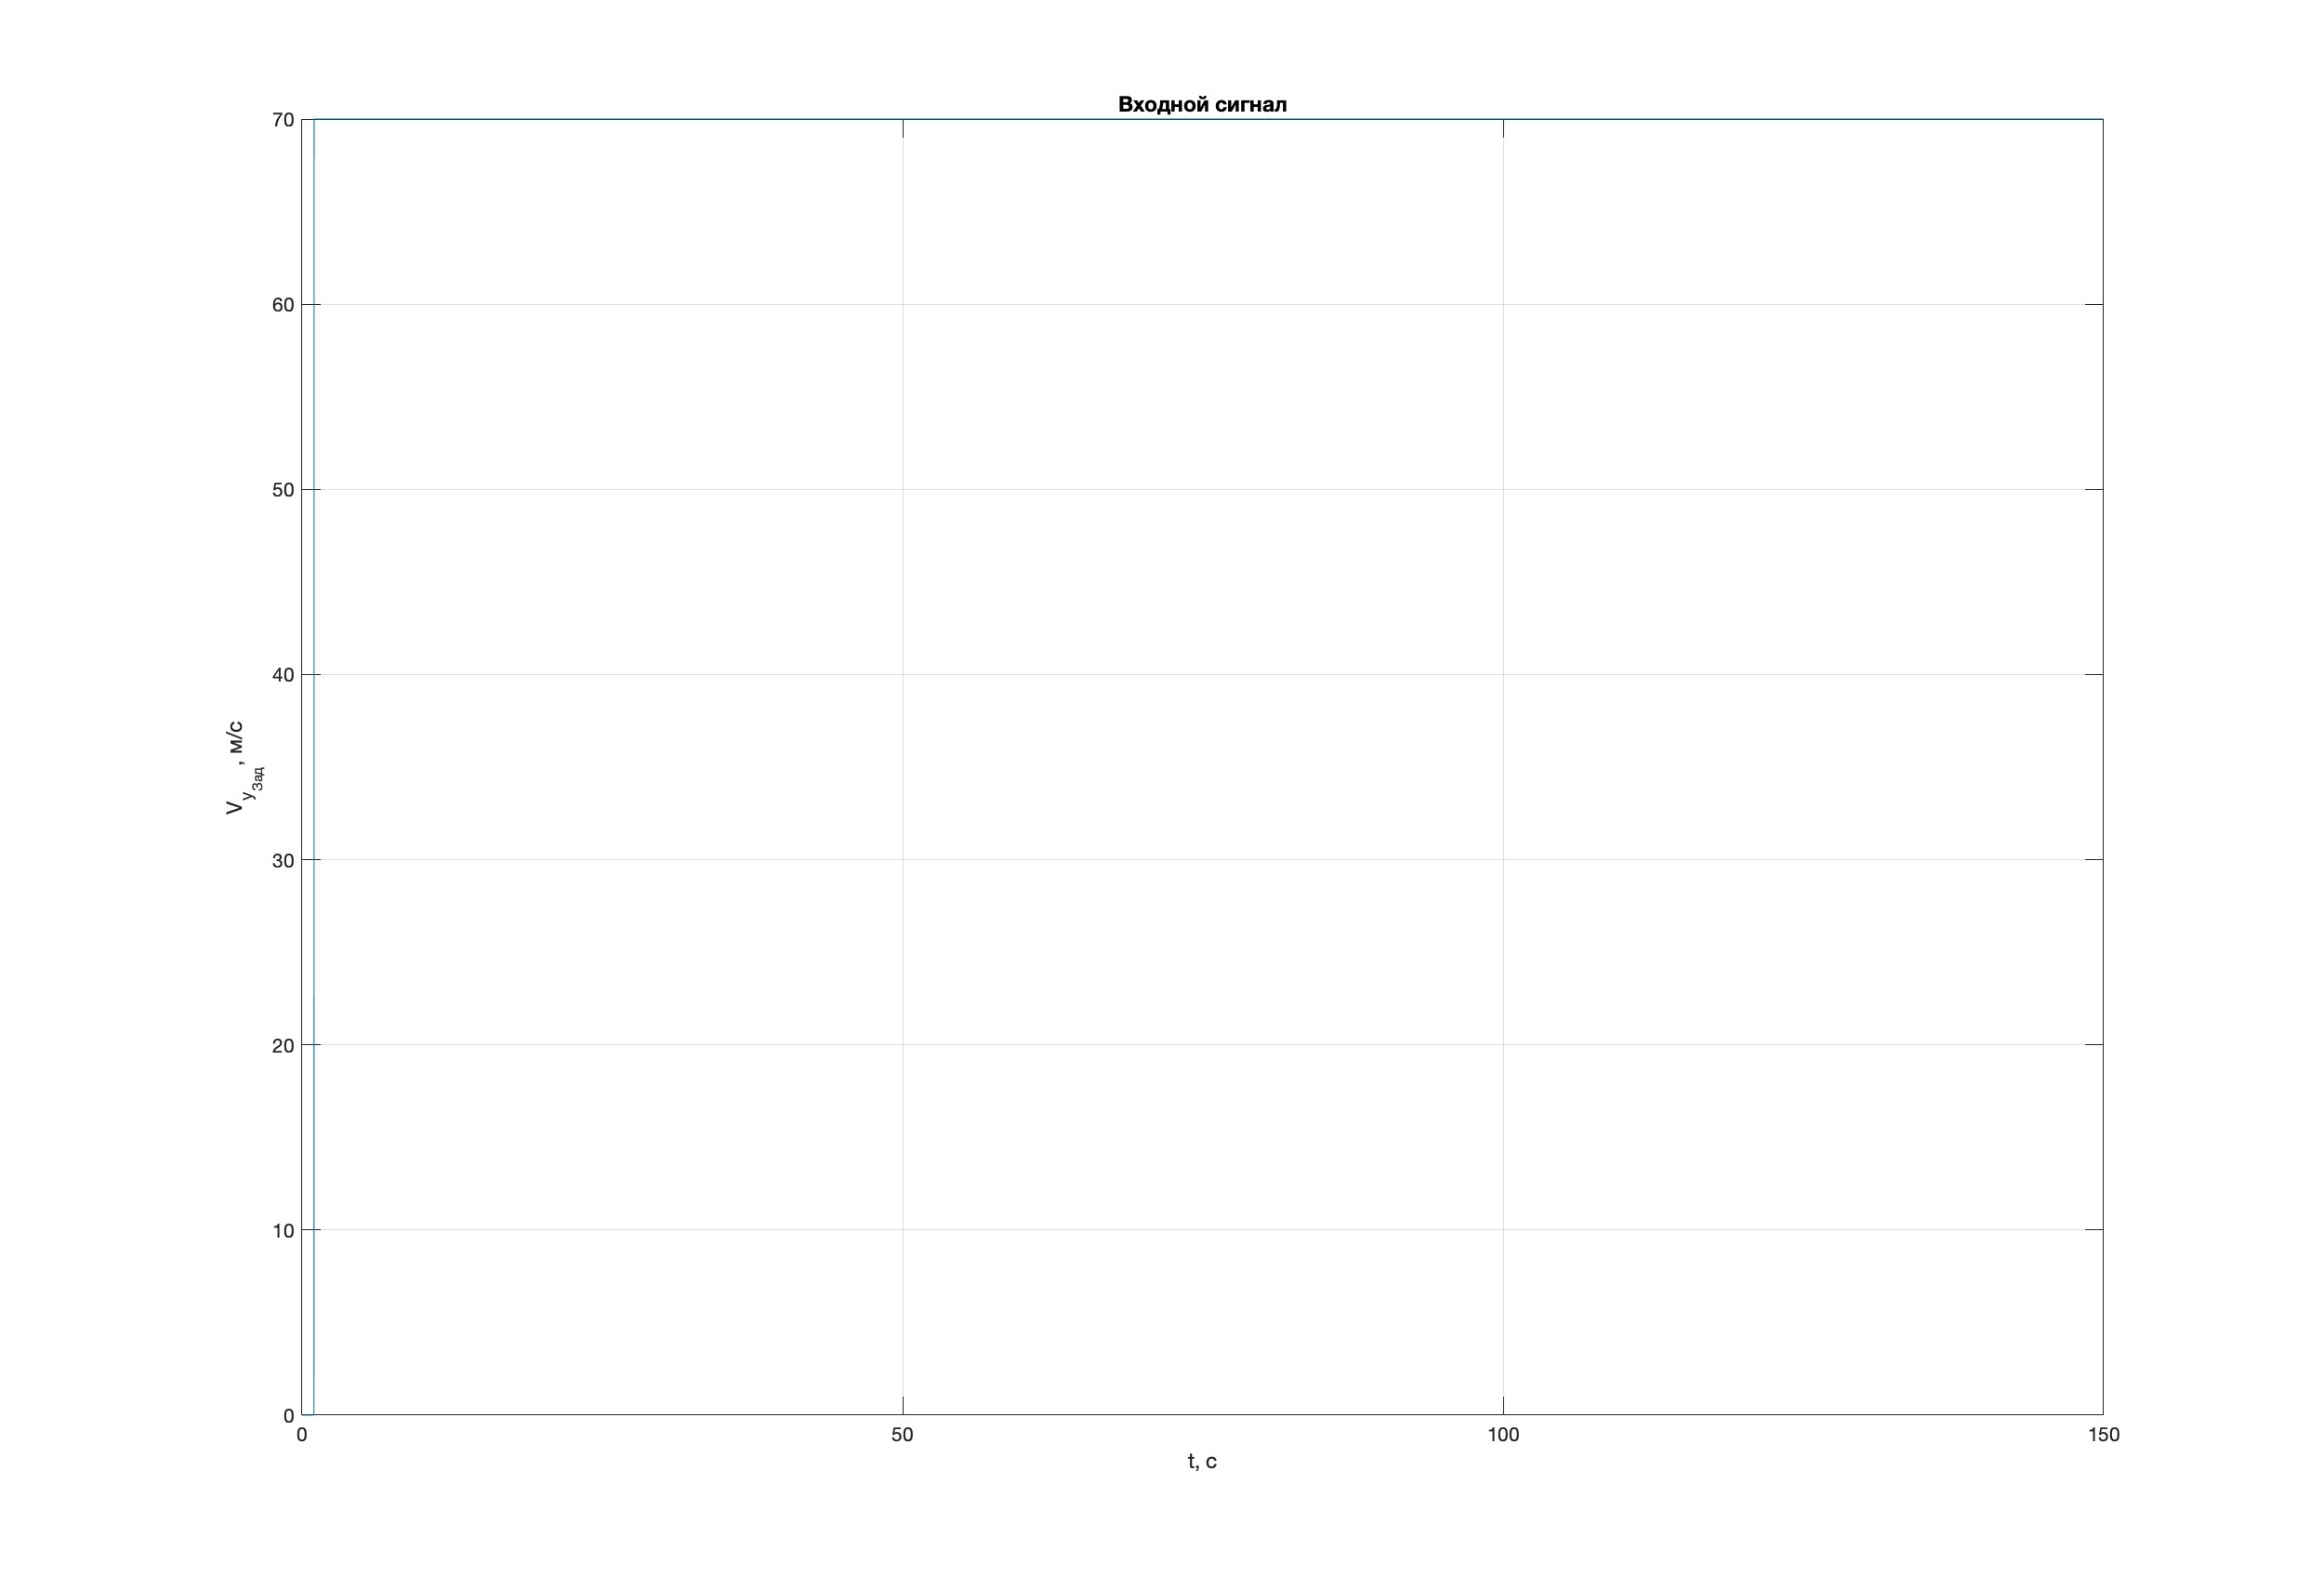
\includegraphics[width=\linewidth]{Оглавление/Part2/Sactions/Content/NotLinFig/Линейный ВС.jpg}}
    \caption{Входной сигнал системы стабилизации вертикальной скорости }
    \label{fig:Входной сигнал системы стабилизации вертикальной скорости}
\end{figure}

\begin{figure}[H]
    \center{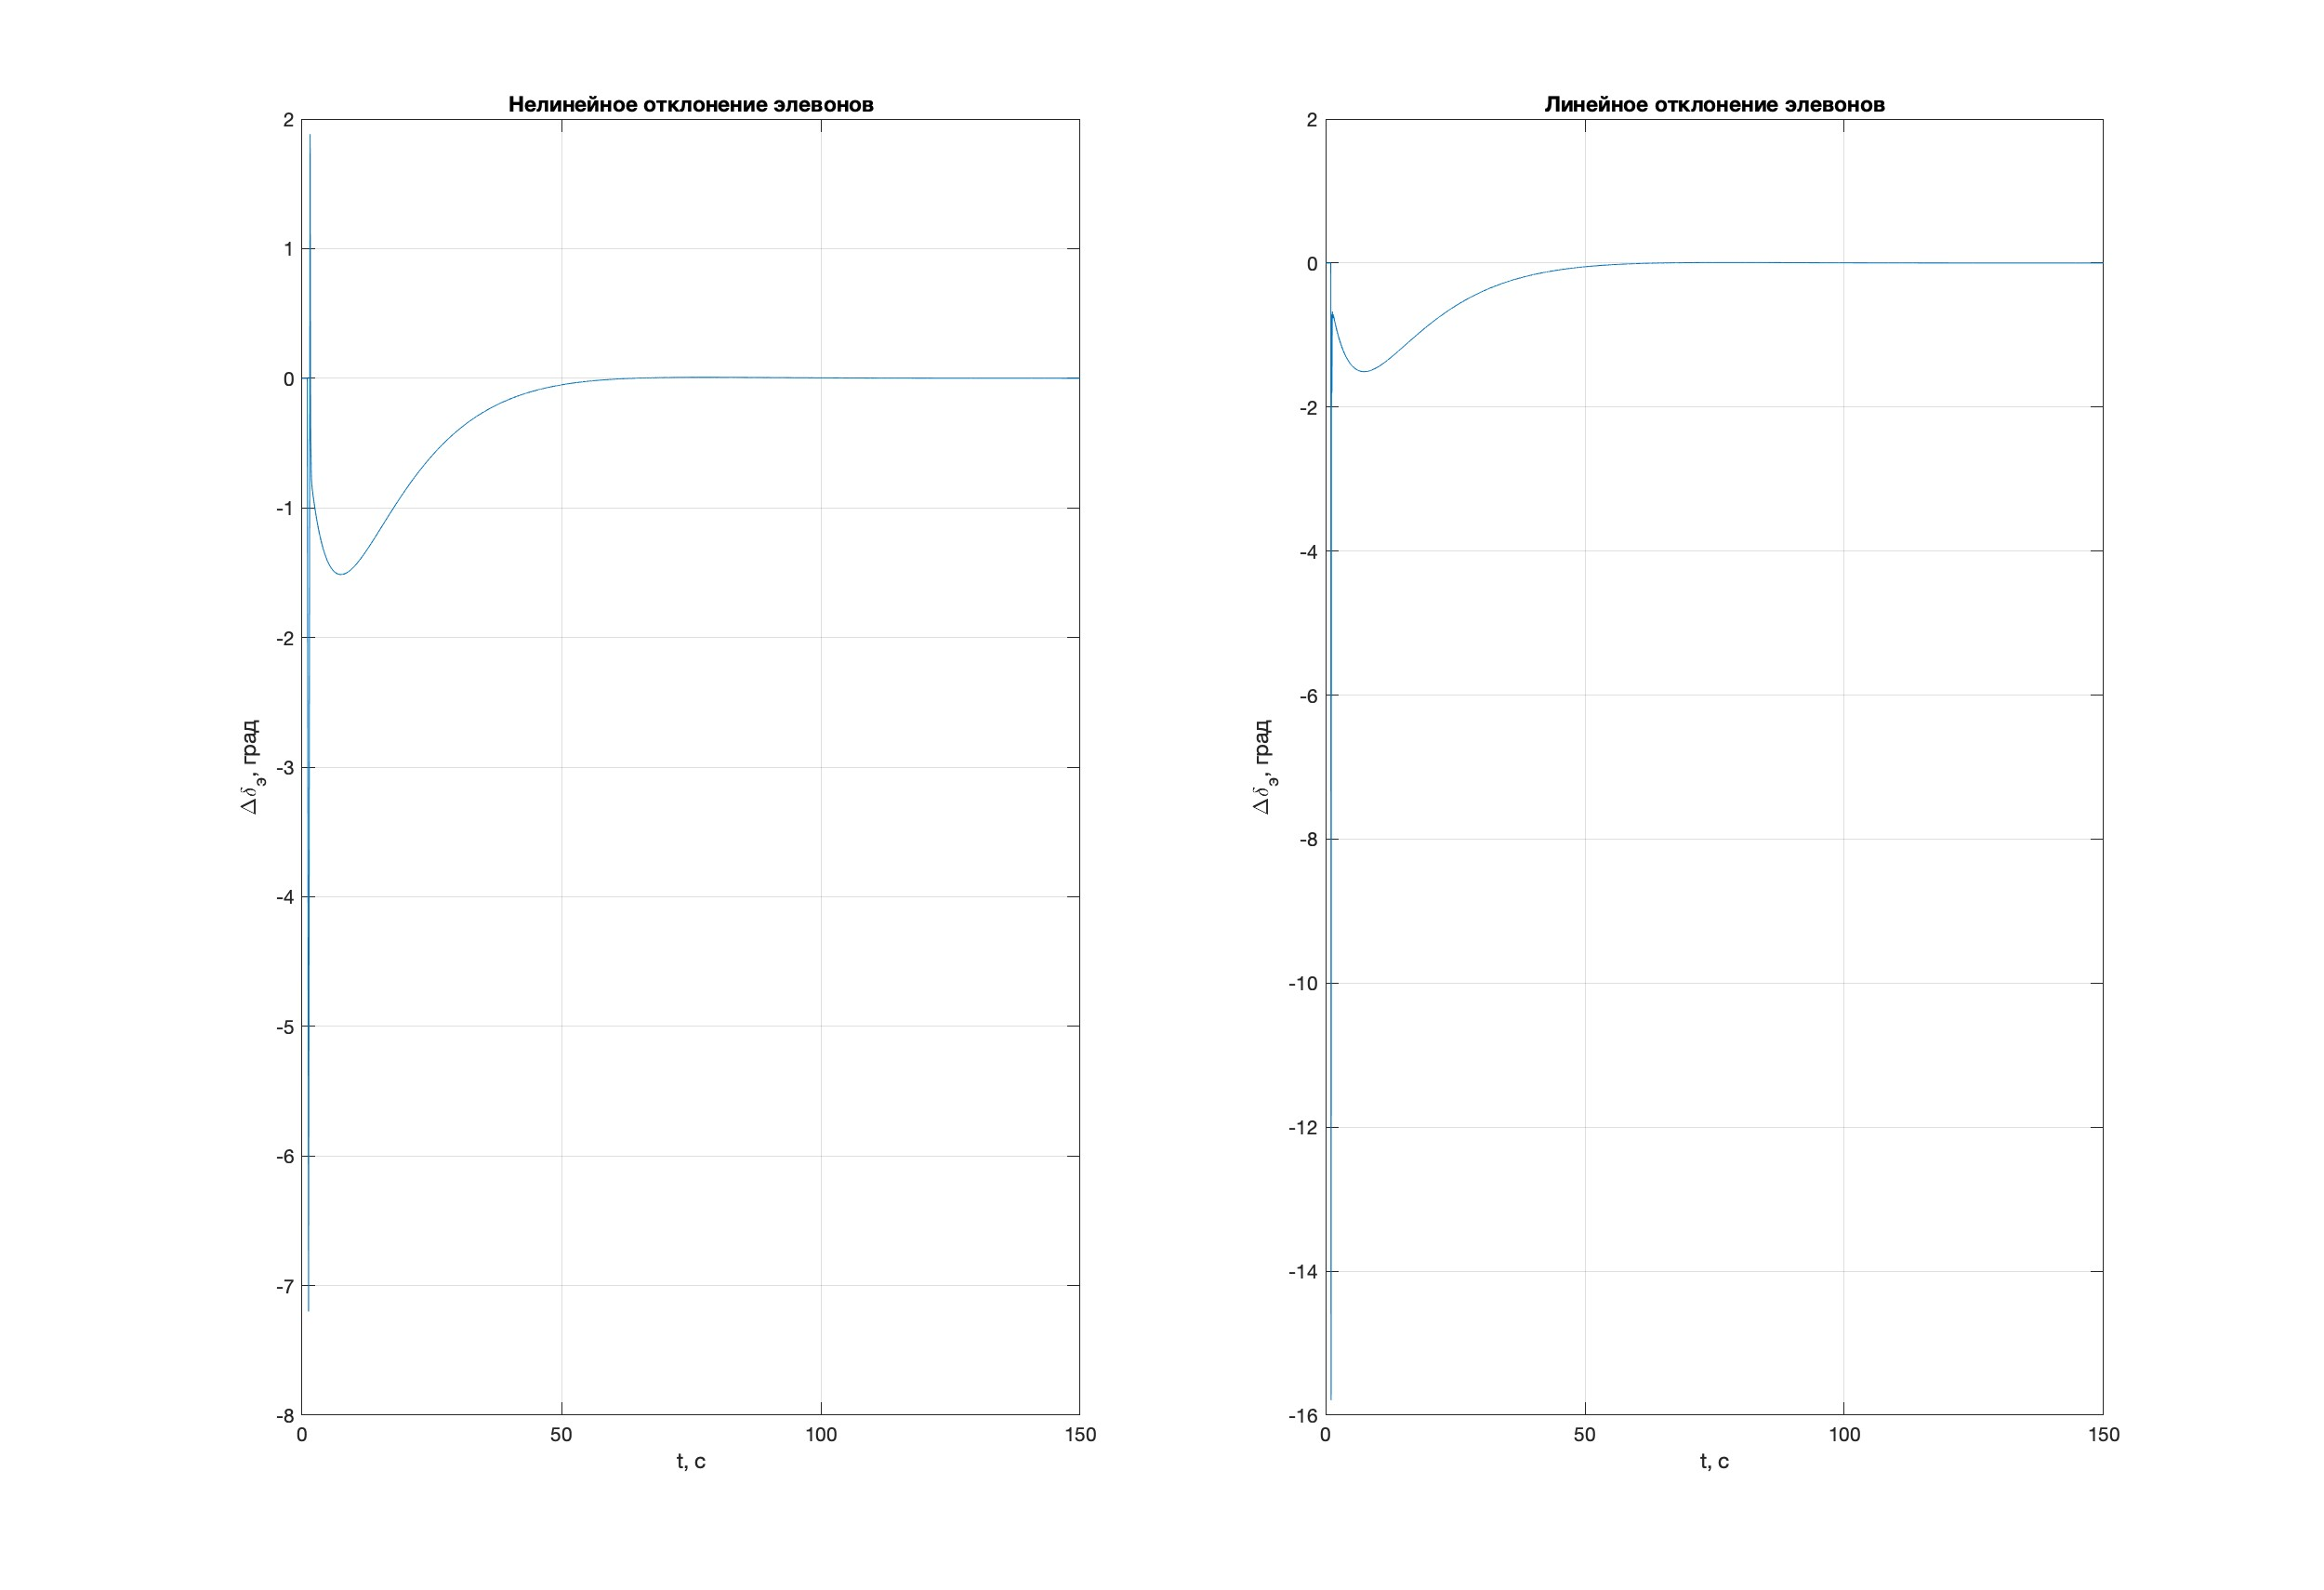
\includegraphics[width=\linewidth]{Оглавление/Part2/Sactions/Content/NotLinFig/Руль.jpg}}
    \caption{Отклонения элевонов для стабилизации угла скольжения}
    \label{fig:Отклонения элевонов для стабилизации угла скольжения}
\end{figure}

\begin{figure}[H]
    \center{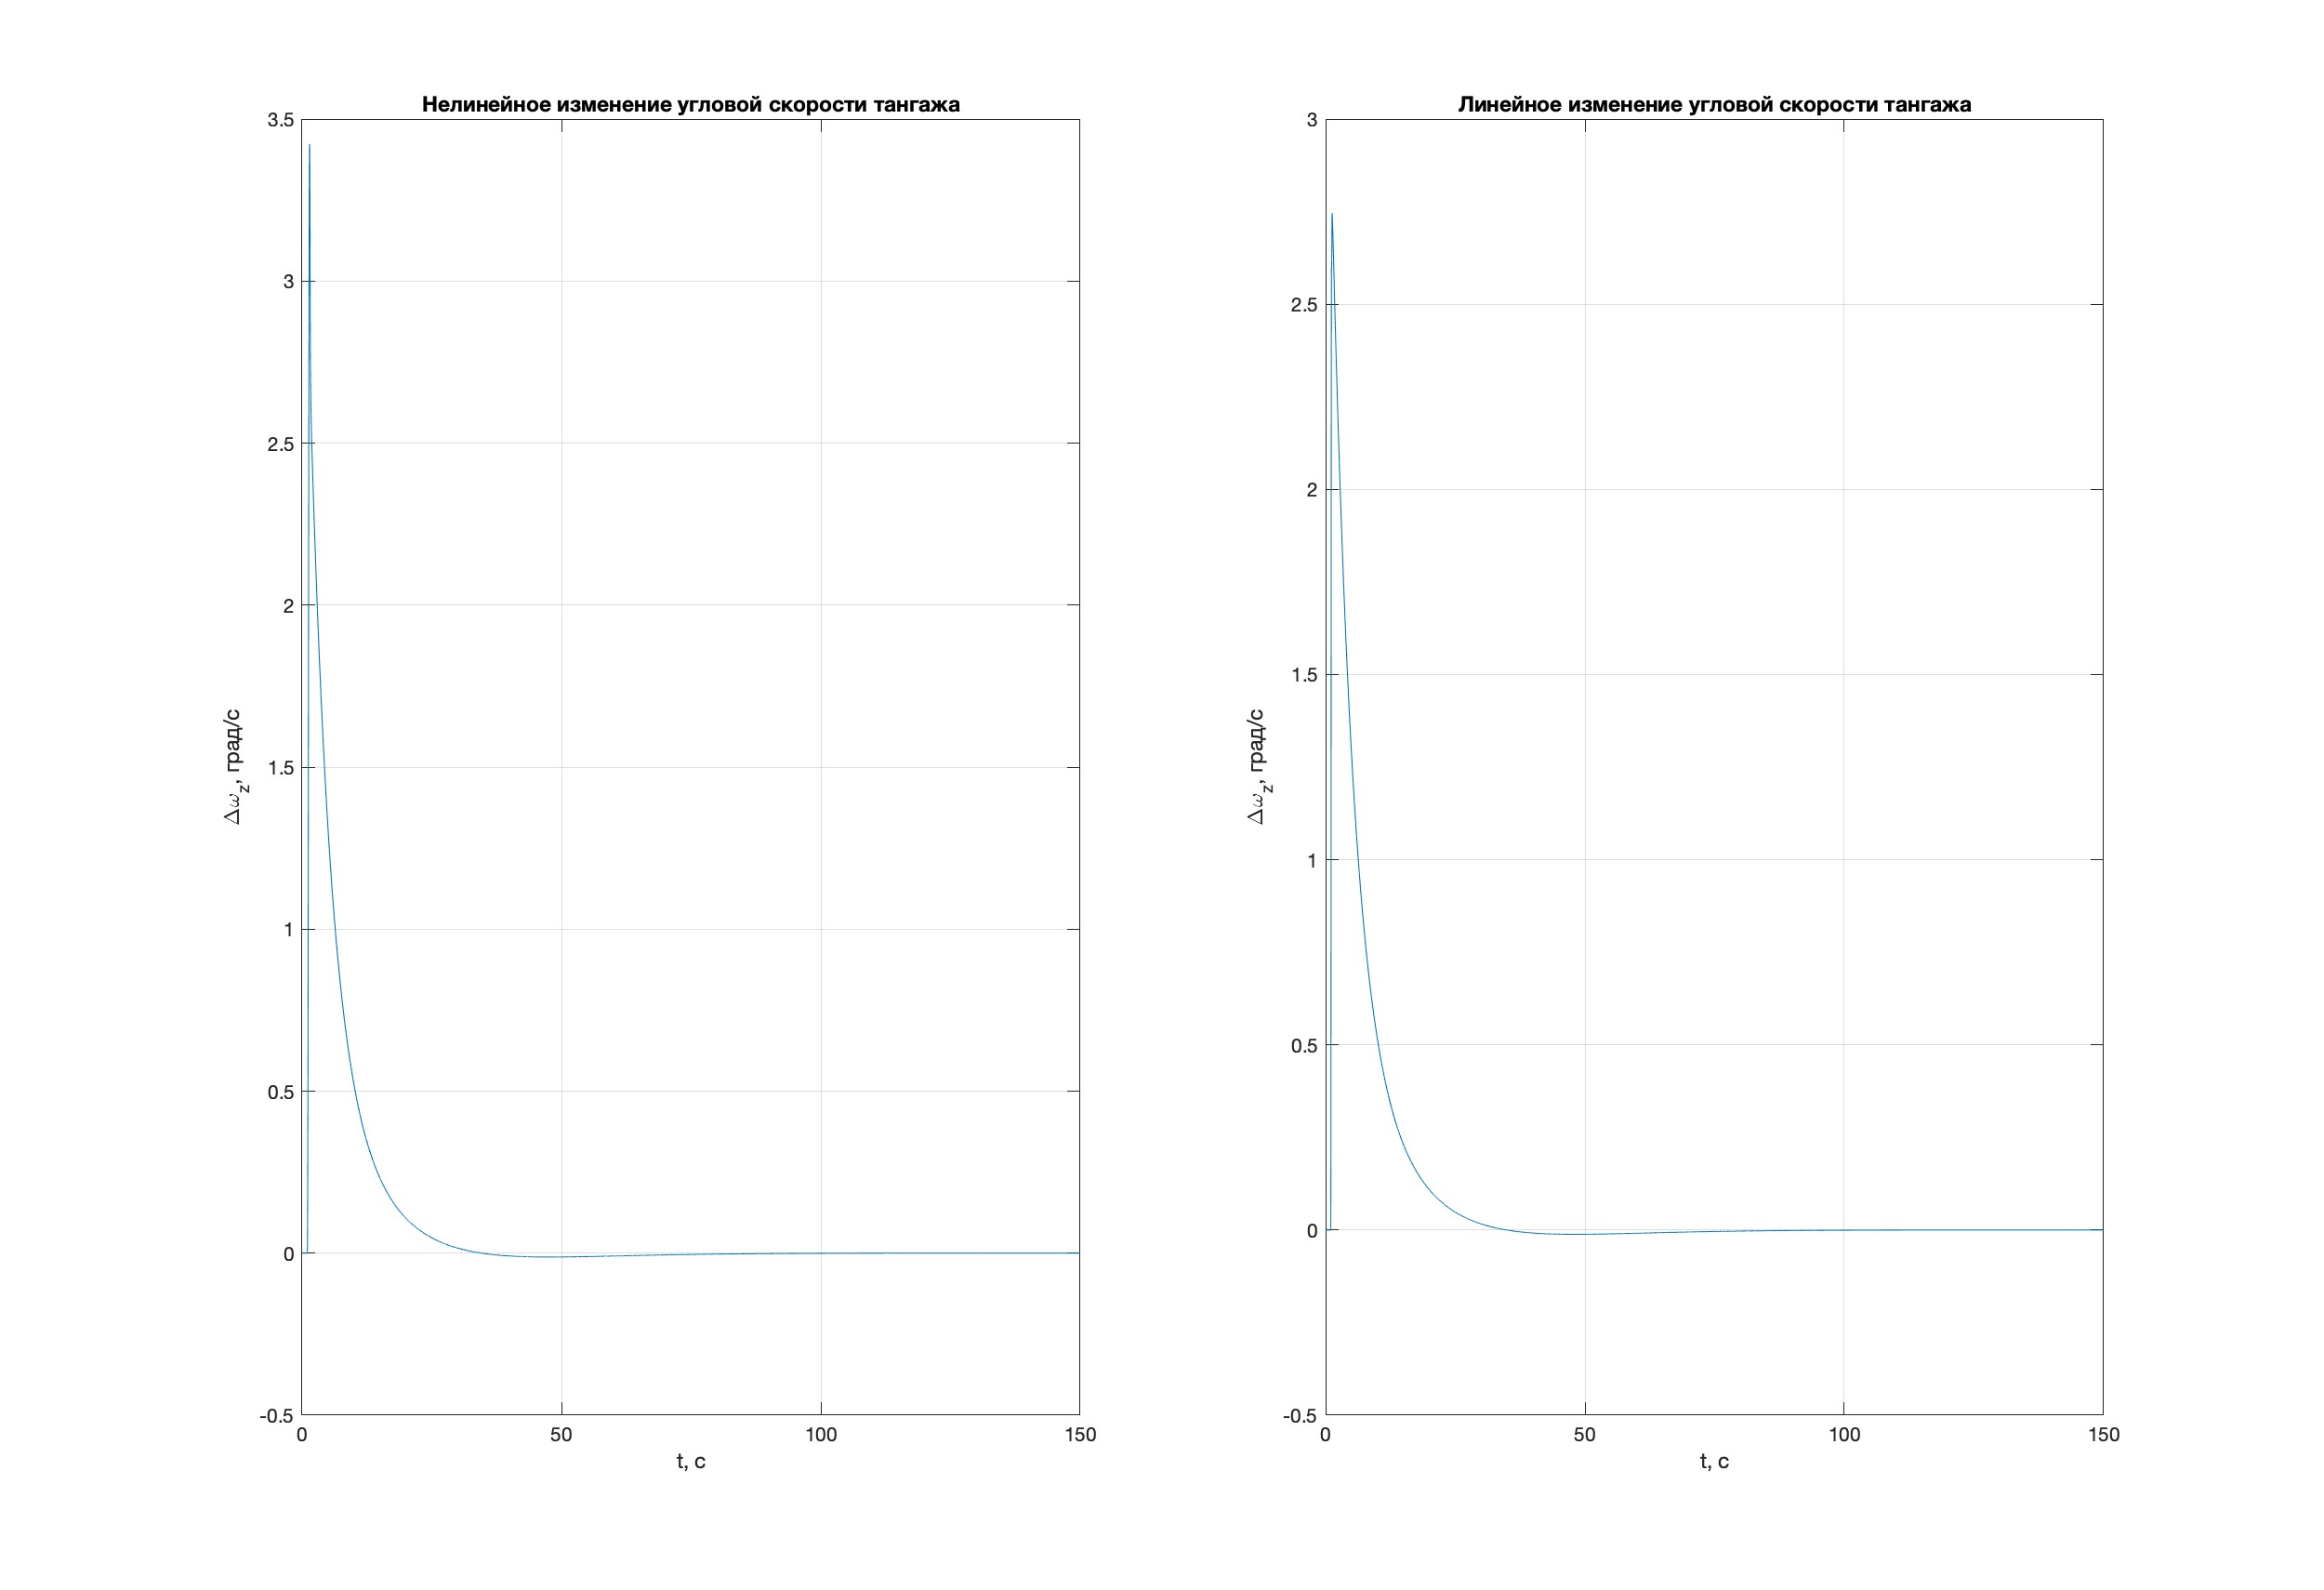
\includegraphics[width=\linewidth]{Оглавление/Part2/Sactions/Content/NotLinFig/wz.jpg}}
    \caption{Изменение угловой скорости тангажа в процессе стабилизации вертикальной скорости}
    \label{fig:Изменение угловой скорости тангажа в процессе стабилизации вертикальной скорости}
\end{figure}

\begin{figure}[H]
    \center{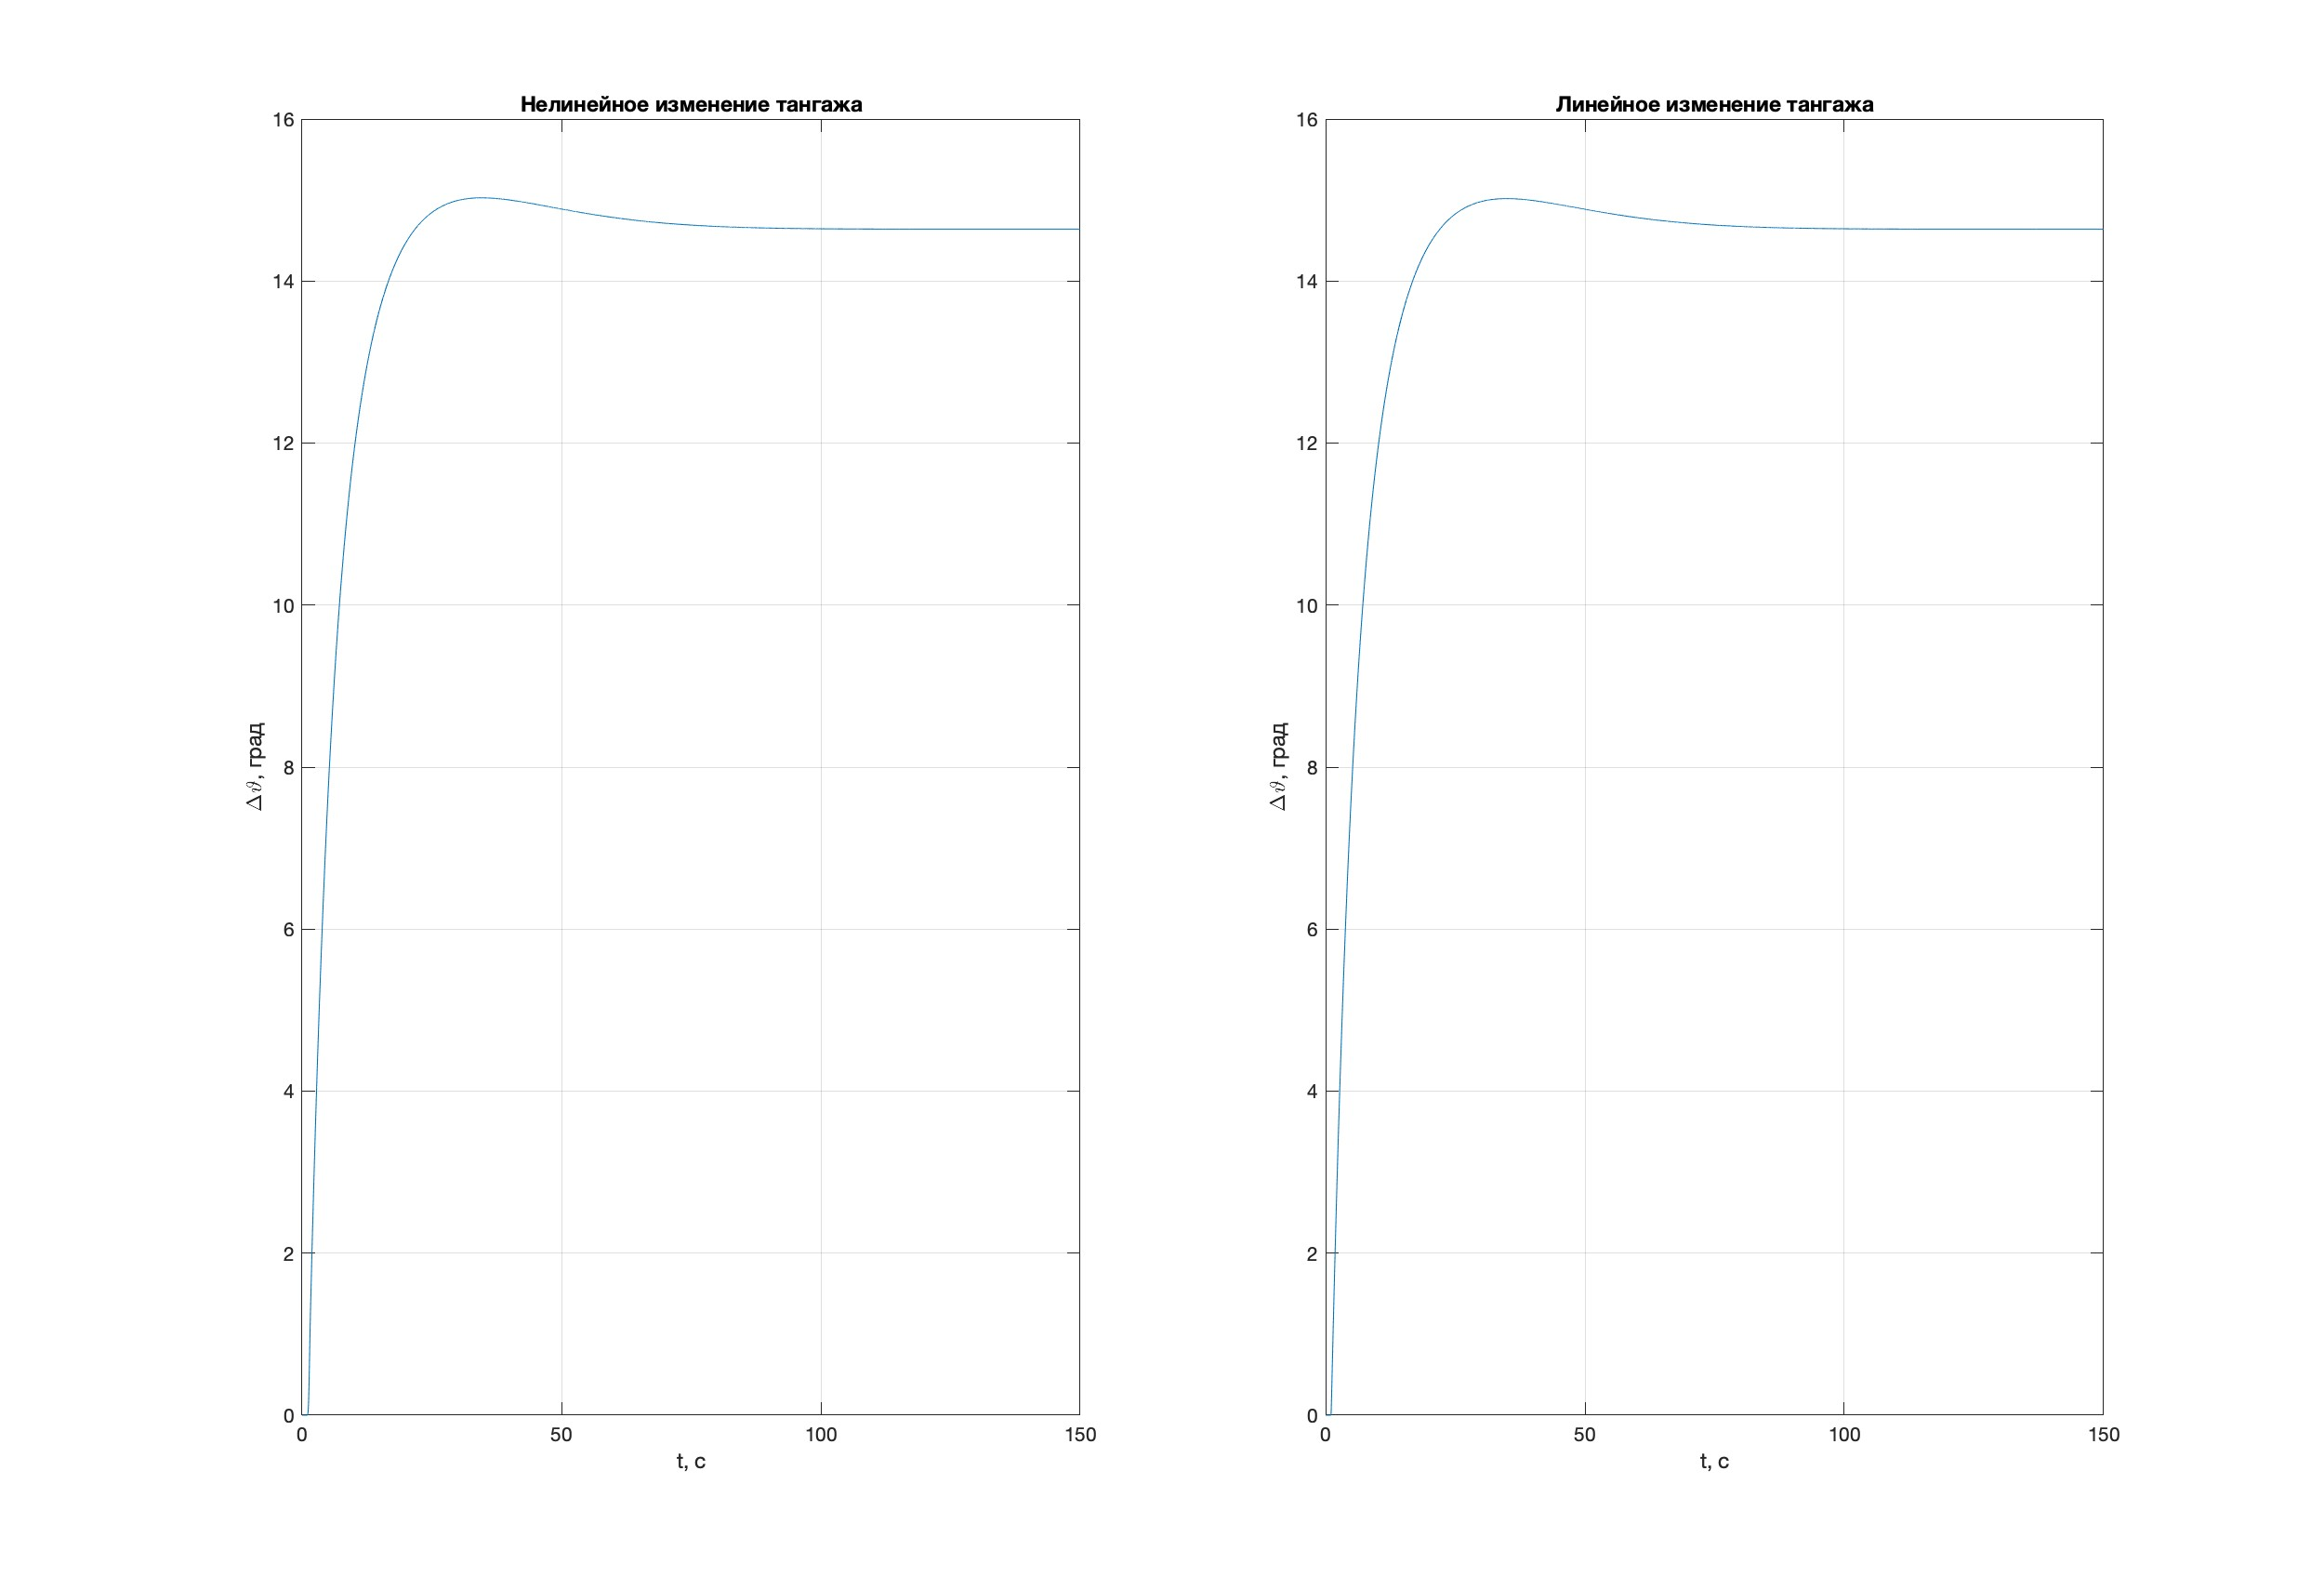
\includegraphics[width=\linewidth]{Оглавление/Part2/Sactions/Content/NotLinFig/vartheta.jpg}}
    \caption{Изменение угла тангажа при стабилизации вертикальной скорости}
    \label{fig:Входной сигнал системы изменения тангажа}
\end{figure}

\begin{figure}[H]
    \center{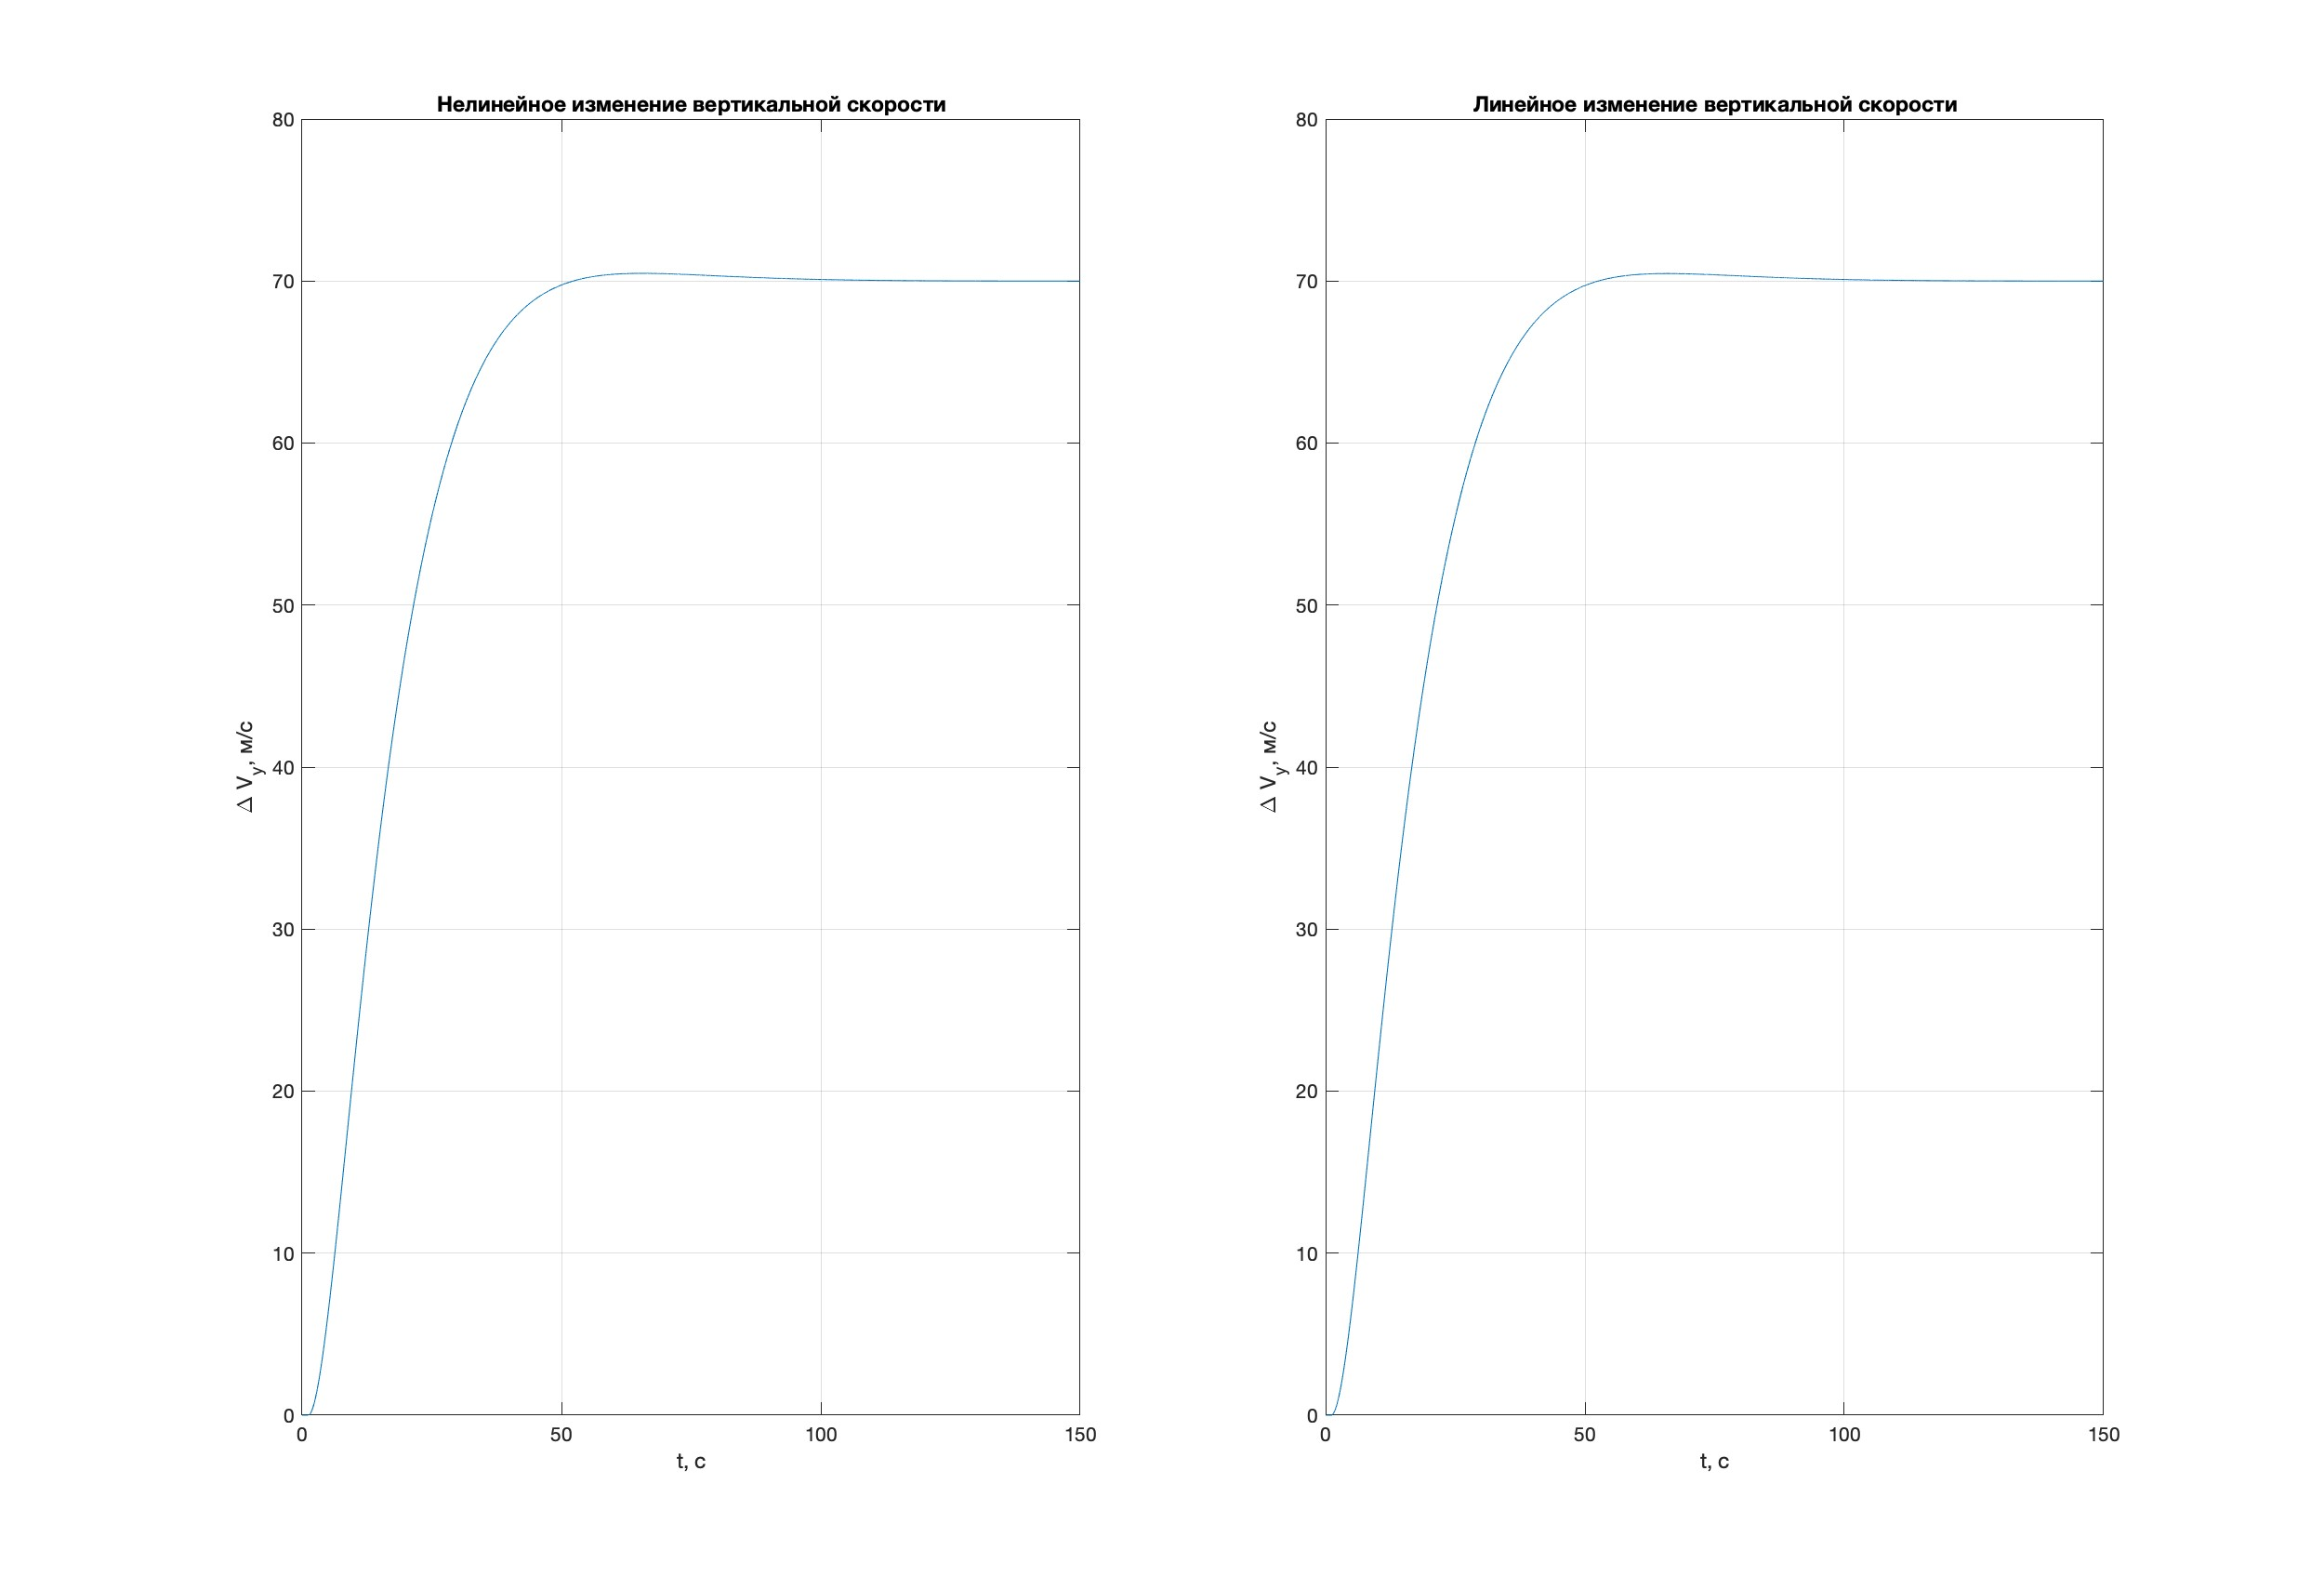
\includegraphics[width=\linewidth]{Оглавление/Part2/Sactions/Content/NotLinFig/Vy.jpg}}
    \caption{Выходной сигнал системы стабилизации вертикальной скорости самолета}
    \label{fig:Входной сигнал системы стабилизации вертикальной скорости}
\end{figure}

%__________________________________________________________________________________________


\begin{center}
    \subsubsubsection{Сравнительный анализ}
\end{center}

Изучив рис.\ref{fig:Отклонения элевонов для стабилизации угла скольжения} можно сделать следующие выводы:
\begin{enumerate}
    \item При введении ограничений на скорость изменения выходного сигнала скорость не превышает 30 град/с что приемлемо, также при введении ограничений на максимальную амплитуду входного и выходного сигналов привод отрабатывает сигнал немного дольше чем без ограничений, «колебательность» сигнала остается одинаковой и в линейном и нелинейном случае.
    \item Также введение ограничений расширяют диапазон заданных значений входного сигнала, то есть при вводе большого значения входного сигнала системы, выходной сигнал привода не превысит значений, указанных в ограничителях, следовательно, при работе системы не произойдет каких-либо неполадок. 
\end{enumerate}
Изучив рис.\ref{fig:Изменение угловой скорости тангажа в процессе стабилизации вертикальной скорости}-\ref{fig:Входной сигнал системы стабилизации вертикальной скорости} можно сделать следующие выводы:

\begin{enumerate}
    \item В линейном и нелинейном случае самолет достигает установившегося значения вертикальной скорости практически за одно и тоже время. 
    \item И в линейной и нелинейной системе вертикальная скорость в конце переходного процесса не равна заданному значению, это связанно с тем, что имеет место быть статическая ошибка. 
\end{enumerate}
\newpage
\section{Специальная часть}
\subsection{Обратная динамика}
\pagestyle{fancy}
\fancyhf{}
\rhead{Дипломная работа}
\lhead{Специальная часть}
\rfoot{\thepage}

Чтобы улучшить пилотажные характеристики и точность пилотирования, возможно синтезировать контроллер на основе 
принципа обратной динамики, который показан в работе {\cite{Zoe}}. Но при использовании данного метода порядок числителя будет выше порядка знаменателя, поэтому необходимо использовать фильтры.

В этой работе мы будем вычислять обратную динамику с помощью обратных связей, т.к. здесь нет необходимости ставить дополнительные фильтры.

\subsection{Исслеуемая модель}

Данная модель была всзята из дисертации {\cite{Diser}}

Основные допущения: 
\begin{enumerate}
    \item Рассмотривается линеаризованная модель короткопериодического движения 
    \item Система исследуется в продольном канале управления
    \item Угол атаки $\alpha$ постоянный и равен $13,7^0$ 
\end{enumerate}

Линейная математическая модель может быть представлена в знакомой форме пространства состояний в виде:
\begin{equation}
    \begin{aligned}
        \dot{x}(t) = Ax(t) + Bu(t) \\
        y(t) = Cx(t) + Du(t)
    \end{aligned}
\end{equation}

Линейная математическая модель может быть представлена в знакомой форме пространства состояний в виде:

\begin{equation}
    \label{eq:Линеаризованная моель СПС}
\begin{bmatrix}
        \dot{V}_x\\ 
        \dot{V}_y\\ 
        \dot{\omega_z}\\ 
        \dot{\theta}
    \end{bmatrix} =
    \begin{bmatrix}
        -0.0110 & 0.0433 & 1.7295 & -7.1876\\ 
        -0.0691 & -0.6975 & -7.0678 & -54.8976\\ 
        0.00011 & 0.00116 & -0.35407 & 0.0911\\ 
        0 & 0 & 1 & 0
    \end{bmatrix} \begin{bmatrix}
        V_x\\ 
        V_y\\ 
        \omega_z \\ 
        \theta
    \end{bmatrix} 
        +\begin{bmatrix}
        -0.4412\\ 
        -12.388\\ 
        -0.58446 \\ 
        0
    \end{bmatrix}  u
\end{equation}

Система ДУ приводит к следующей краткой аэродинамической и управляющей производной:

\begin{equation}
    \label{eq:Линеаризованная моель СПС}
\begin{bmatrix}
        \dot{V}_x\\ 
        \dot{V}_y\\ 
        \dot{\omega_z}\\ 
        \dot{\theta}
    \end{bmatrix} =
    \begin{bmatrix}
        x_{V_x}& x_{V_y}&x_{\omega_z} &x_{\theta} \\ 
        z_{V_x}&z_{V_w} &z_{\omega_z} &z_\theta \\ 
        m_{V_x}&m_{V_y} &m_{\omega_z} &m_\theta \\ 
        0& 0& 1&0 
    \end{bmatrix} \begin{bmatrix}
        V_x\\ 
        V_y\\ 
        \omega_z \\ 
        \theta
    \end{bmatrix} 
        +\begin{bmatrix}
        x_{\delta_\text{э}}\\ 
        z_{\delta_\text{э}}\\ 
        m_{\delta_\text{э}}\\ 
        0
    \end{bmatrix} \delta_\text{э} 
\end{equation}

Относительные величины и знаки кратких аэродинамических
производных относительного момента тангажа, $m_{V_x}$, $m_{V_y}$, $m_{\omega_z}$ и $m_\theta$, важны для устойчивости и динамических свойств
самолета. Отмечая следующее:
\begin{itemize}
\item Член производной относительной момента по скорости, $m_{V_x}$, положительный из-за того, что центральная линия тяги расположена
ниже вертикального положения центра тяжести. Однако он очень мал (0,00011) и поэтому мало повлияет на стабильность системы.
\item Момент относительной производной по вертикальной скорости, $m_{V_y}$ хотя и небольшая, является положительной, что указывает на статически
неустойчивый самолет.
\item Величина производной относительного демпфирующего момента, $m_{\omega_z}$, невелика, хотя и отрицательна и стабилизирует систему.
\end{itemize}

Входная матрица преобразует отрицательный (вверх) входной сигнал элевона в положительный момент шага, нормальную и осевую силу.

\subsubsection{Передаточные функции систему ДУ}

Зная систему дифференциальных уравнений ({\ref{eq:Линеаризованная моель СПС}}), найдём передаточные функции 

\begin{equation}
    \label{eq:ПФ по горизонтальной скорости СПС}
    \{ \frac{V_x}{\delta_\text{э}} \} = \frac{-0.4412p^3 - 2,011p^2 + 3.388p + 4.471}{p^4 + 1.063p^3 + 0.1784p^2 + 0.003833p + 3.424 \cdot 10^{-5}}
\end{equation}

\begin{equation}
    \label{eq:ПФ по вертикальной скорости СПС}
    \{ \frac{V_y}{\delta_\text{э}} \} = \frac{-12.39^3 - 0.3612p^2 + 33.29p + 0.06517}{p^4 + 1.063p^3 + 0.1784p^2 + 0.003833p + 3.424 \cdot 10^{-5}}
\end{equation}

\begin{equation}
    \label{eq:ПФ по угловой скорости тангажа СПС}
    \{ \frac{\omega_z}{\delta_\text{э}} \} = \frac{-0.5845p^3 - 0.4285p^2 - 0.006449p - 3.57 \cdot 10^{-20}}{p^4 + 1.063p^3 + 0.1784p^2 + 0.003833p + 3.424 \cdot 10^{-5}}
\end{equation}

\begin{equation}
    \label{eq:ПФ по углу наклона траектории}
    \{ \frac{\theta}{\delta_\text{э}} \} = \frac{-0.5845p^2 - 0.4285p - 0.006449}{p^4 + 1.063p^3 + 0.1784p^2 + 0.003833p + 3.424 \cdot 10^{-5}}
\end{equation}

\subsection{План исследований}
\subsubsection{Обратная динамики }
Обратная динамика вычислена через обратные связи как показанно на рис.\ref{fig:САУ_ОД}
\begin{figure}[H]
    \centering 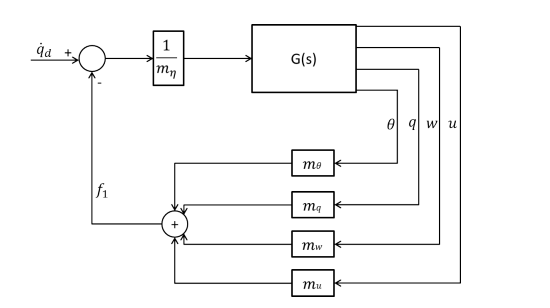
\includegraphics[width=15cm,height=10cm]{Оглавление/Part3/figures/САУ_ОД.png}
    \caption{Реализация динамической инверсии}
    {\label{fig:САУ_ОД}}
    \end{figure}
\subsection{Изучение робастности} 

Чтобы изучать робастность контроллера на основе обратной динамики, мы проводили  с разными моделями продольного движения разных самолётов. 

\subsubsection{Модель (European SPS)} 
    \begin{bmatrix}
        -0.0110 & 0.0433 & 1.7295 & -7.1876\\ 
        -0.0691 & -0.6975 & -7.0678 & -54.8976\\ 
        0.00011 & 0.00116 & -0.35407 & 0.0911\\ 
        0 & 0 & 1 & 0
    \end{bmatrix} \cdot X=\begin{bmatrix}
        -0.4412\\ 
        -12.388\\ 
        -0.58446 \\ 
        0
    \end{bmatrix} \cdot U=\dot{X}
\begin{center}
    Эксперименты с изменениями А и В
\end{center}

Суть данного эксперимента заключается в проверке характеристик надежности системы при изменении матрицы входных параметров $B$. Результаты эксперимента можно кратко изложить ниже.
    
\begin{figure}[H]
    \centering 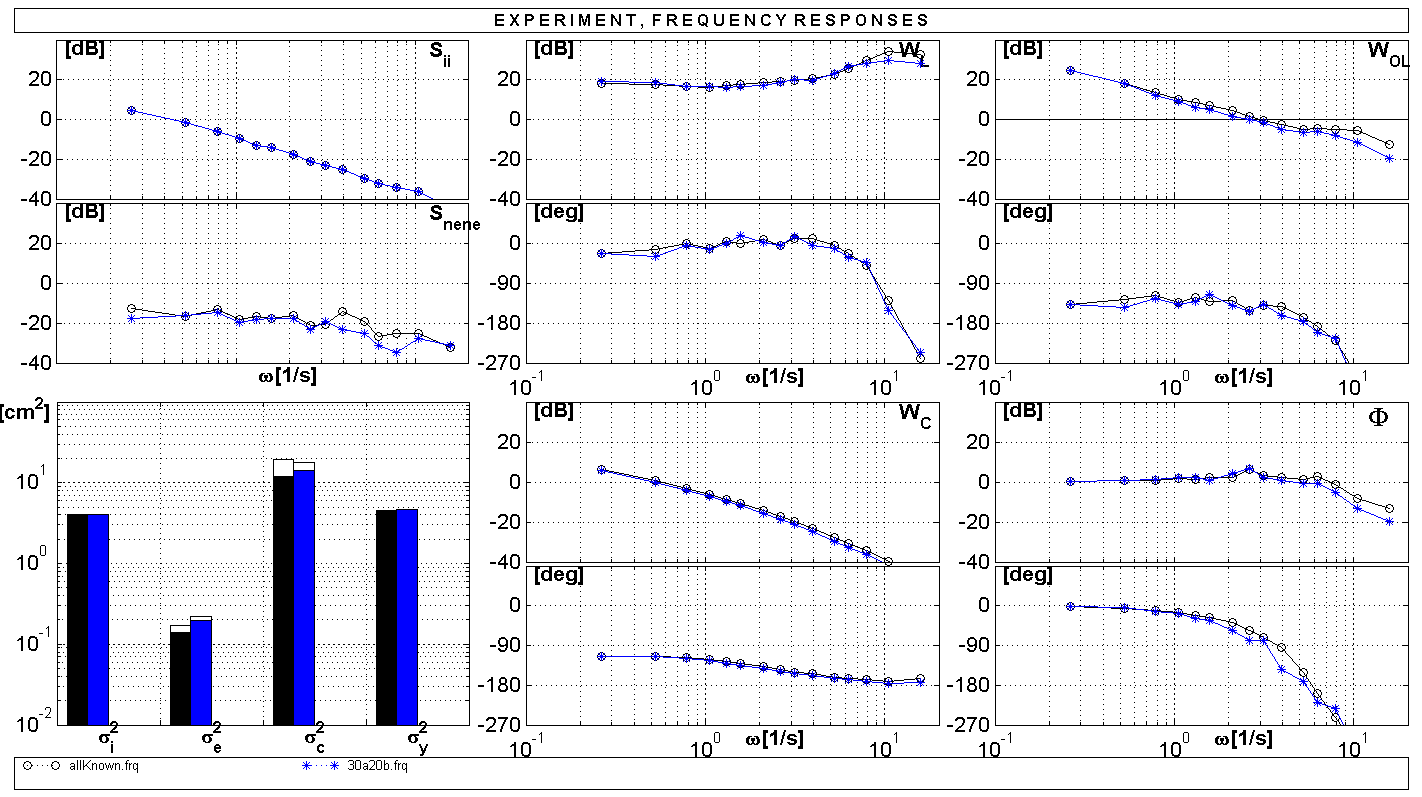
\includegraphics[width=17cm,height=15cm]{Оглавление/Part3/figures/chast2_20A30B.png}
    \caption{}
    {\label{fig:Частотки второй Системы с изменением А и В}}
    \end{figure}

    \begin{center}
        Эксперимент без PI 
    \end{center}



    Также мы подразумеваем, что мы имеем дело с $K_\text{ш} = -0,6$

    Из Рис. {\ref{fig:Результаты экспериментов без PI}}
    \begin{itemize}
        \item [-] c увеличением неточности знаний увеличивается $\sigma_e^2$
        \item [-] лётчик вводит меньшие усилия на ручку управления $\sigma^2_c$ 
        \item [-]  Я ещё ничего не приумал   
    \end{itemize}

\newpage
        \addcontentsline{toc}{section}{Список литературы}  
\begin{thebibliography}{10}
    \bibitem{Album}
    Альбом исходный данных кафедры 106. Часть 1 и часть 2   
    \bibitem{EfremovBig}
    А.Е. Ефремов, В.Ф. Захарченко, В.Н. Овчаренко др. «Динамика полёта»
    \bibitem{UDLA}
    Ю.П.Гуськов, Г.И.Загайнов «Управление полетом самолетов»
    \bibitem{GOST}
    Национальный стандарт атмосферы ГОСТ 4401-81
    \bibitem{Zoe}
    Zoe Mbikayi, Alexandr V. Efremov, Yury V. Tiumentsev Moscow Aviation Institute, Moscow, 125080 "Framework for application of linear control methods to nonlinear  flight control"
\end{thebibliography}

\end{document}  % КОНЕЦ ДОКУМЕНТА !

